\documentclass[11pt,letterpaper]{report}

\usepackage{amsmath}
\usepackage{amsfonts}
\usepackage{amssymb}
\usepackage{graphicx}
\usepackage{tabularx}
\usepackage{algorithm}
\usepackage{algpseudocode} 
\usepackage{subcaption}
\usepackage[font=small]{caption}


%\usepackage[backref]{hyperref}
\usepackage{url}
\usepackage[english]{babel}
\usepackage{setspace} 
\usepackage[margin=1in]{geometry}

\usepackage{cjhebrew}
%\usepackage{times}
%\usepackage{venturis2}

\doublespacing

\title{\textsc{Towards a Framework for DHT Distributed Computing}}
\author{\textsc{Andrew Benjamin Rosen}}
\date{}

\begin{document}
	
	

	\pagestyle{empty}

	\begin{center}
		%	\includegraphics[width=0.15\textwidth]{example-image-1x1}\par\vspace{1cm}
		{\scshape Towards a Framework for DHT Distributed Computing\par}
		\vspace{0.5cm}
		{by\par}
		\vspace{0.5cm}
		{\scshape Andrew Benjamin Rosen\par}
		\vspace{0.5cm}
		{Under the Direction of Dr.~Anu G.~Bourgeois, PhD \par}
		\vspace{0.5cm}
		{\scshape Abstract \par}
		
	\end{center}
	
	
		Distributed Hash Tables (DHTs) are protocols and frameworks used by peer-to-peer (P2P) systems.
		They are used as the organizational backbone for many P2P file-sharing systems due to their scalability, fault-tolerance, and load-balancing properties.
		These same properties are highly desirable in a distributed computing environment, especially one that wants to use heterogeneous components.
		
		We show that DHTs can be used not only as the framework to build a P2P file-sharing service, but as a P2P distributed computing platform.
		We propose creating a P2P distributed computing framework using distributed hash tables, based on our prototype system ChordReduce.
		This framework would make it simple and efficient for developers to create their own distributed computing applications.
		Unlike Hadoop and similar MapReduce frameworks, our framework can be used both in both the context of a datacenter or as part of a P2P computing platform.  
		This opens up new possibilities for building platforms to distributed computing problems.
		
		One advantage our system will have is an autonomous load-balancing mechanism.
		Nodes will be able to independently acquire work from other nodes in the network, rather than sitting idle.
		More powerful nodes in the network will be able use the mechanism to acquire more work, exploiting the heterogeneity of the network.
		
		By utilizing the load-balancing algorithm, a datacenter could easily leverage additional P2P resources at runtime on an as needed basis.
		Our framework will allow MapReduce-like or distributed machine learning platforms to be easily deployed in a greater variety of contexts.
		
		\vfill
		

		% Bottom of the page
		{\textsc{Index Words}: Distributed Hash Tables, P2P, Voronoi, Delaunay, Networking}
	
	
	\newpage 
	\begin{titlepage}
		
		\begin{center}
			%	\includegraphics[width=0.15\textwidth]{example-image-1x1}\par\vspace{1cm}
			{\scshape Towards a Framework for DHT Distributed Computing\par}
			\vspace{5cm}
			{by\par}
			\vspace{5cm}
			{\scshape Andrew Benjamin Rosen\par}
			
			\vfill
			A Dissertation Submitted in Partial Fulfillment of the Requirements for the Degree of\\
			Doctor of Philosophy in Computer Science\\
			in the College of Arts and Sciences\\
			Georgia State University\\
			2016
		\end{center}
	\end{titlepage}
	
	
	
	
	
	
	\null\vfill
	\begin{center}
		
		Copyright by \\
		Andrew Benjamin Rosen\\
		\begin{cjhebrew}
			.hnwK
		\end{cjhebrew}\\
		2016
	\end{center}
	\newpage
	


	\begin{center}
		{\scshape Towards a Framework for DHT Distributed Computing\par}
		\vspace{5cm}
		{by\par}
		\vspace{5cm}
		{\scshape Andrew Benjamin Rosen\par}
	\end{center}
	\vfill
	\hfill\begin{tabular}{rl}
		Committee Chair & Anu G. Bourgeois \\ 
		&  \\ 
		Committee & Robert Harrison  \\ 
		& Zhipeng Cai
		\\ 
		& Michael Stewart 
	\end{tabular} 
	
	
	\noindent
	Electronic Version Approved:\\
	\vspace{1cm}
	
	\noindent
	Office of Graduate Studies \\
	College of Arts and Sciences \\
	Georgia State University\\
	May 2016 
	
	\newpage
	\pagestyle{plain}
	\pagenumbering{roman}
	
	\chapter*{Dedication}
	To Annie-Rae Rosen, without whom, I would not be who I am today.
	\\
	To my mother, who understands the power of names.
	Whenever I doubted myself, I only had to remember my name and what it meant.
	
	\chapter*{Acknowledgments}	
	There were some people who cared about what I did.  
	I'm not particularly sure why.
	
	
	\setcounter{tocdepth}{4}
	
	%\cleardoublepage
	%\addcontentsline{toc}{chapter}{\listtablename}
	%\addcontentsline{toc}{chapter}{\listfigurename}
	\tableofcontents
	\listoftables
	\listoffigures
	\newpage
	

	\clearpage
	\pagenumbering{arabic}
	\chapter{Introduction}
\label{chapter:intro}
% % % layout
% % % Distributed Computing Challenges
% % % Qualities of DHTs
% % % Hypothesis = These Problems + These qualiteies -> solution
% % % Framework of what these solutions are and what they can do


Distributed Hash Tables (DHTs) are protocols and frameworks used by peer-to-peer (P2P) systems.
They are used as the organizational backbone for many P2P file-sharing systems due to their scalability, fault-tolerance, and load-balancing properties.
These same properties are highly desirable in a distributed computing environment, especially one that wants to use heterogeneous components.
We will show that DHTs can be used not only as the framework to build a P2P file-sharing service, but a more generic distributed computing platform.


% What do I want to do?
\section{Objective}
Our goal is to create a framework to further generalize Distributed Hash Tables (DHTs) to be used for distributed computing.
Distributed computing platforms need to be scalable, fault-tolerant, and load-balancing.
%The ability to incorporate heterogeneous hardware is a definite benefit.
We will discuss what each of these mean and why they are important in section \ref{sec:challenges}, but briefly:

\begin{itemize}
	\item The system should be able to work effectively no matter how large it gets.
	As the system grows in size, we can expect the overhead to grow in size as well, but at an extremely slower rate.
	\item The more machines integrated into the system, the more we can expect to see hardware failures.
	The system needs to be able to automatically handle these hardware failures.
	\item Having a large number of machines to use is worthless if the amount of work is divided unevenly among the system.
	The same is true if the system hands out larger jobs to less powerful machines or smaller jobs to the more powerful machines.
	%\item We cannot assume that we be able to replace our broken machines with exact replicas, nor do we assume we would want to. 
\end{itemize}


These are many of the same challenges that Peer-to-peer (P2P) file sharing applications have.
Many P2P applications use DHTs to address these challenges, since DHTs are designed with these problems in mind.
We propose that DHTs can be used to create P2P distributed computing platforms that are completely decentralized.
%Rather than keys being assigned to some data, we can assign keys to tasks and automatically distribute those tasks to the responsible nodes
There would be no need for some central organizer or scheduler to coordinate the nodes in the network.
Our framework would not be limited to only a P2P context, but could be applied in data centers, a normally centrally organized context.


A successful DHT-based computing platform would need to address the problem of dynamic load-balancing.
This is currently an unsolved\footnote{As far as we know.} problem. %I have to check a couple of papers of to confirm.
If an application can dynamically reassign work to nodes added at runtime, this opens up new options for resource management.
Similarly. if a distributed computation  is running too slow, new nodes can be added to the network during runtime or idle nodes can boot up more virtual nodes. %(now that I think of it this is two different but highly related problems: internal and external).

%Move this bit to the end?
Chapter \ref{chapter:background} will delve into how DHTs work and examine specific DHTs.
The remainder of the dissertation will then discuss the work we have completed and plan on doing to demonstrate the viability of using DHTs for distributed computing and other non-traditional tasks.



% How I will do it is in the experiments chapter

% Why should you care?
\section{Applications of Distributed Hash Tables}

Distributed Hash Tables have been used in numerous applications:

\begin{itemize}
	\item \textit{P2P file sharing} is by far the most prominent use of DHTs.  
	The most well-known application is BitTorrent \cite{bittorrent}, which is built on Mainline DHT \cite{mainline}.
	\item DHTs have been used for \textit{distributed storage} systems \cite{CFS}.
	\item \textit{Distributed Domain Name Systems} (DNS) have been built upon DHTs \cite{cox2002serving} \cite{pappas2006comparative}.
	Distributed DNSs are much more robust that DNS to orchestrated attacks, but otherwise require more overhead.
	%\item Distributed search (faroo)
	\item DHT was used as the name resolution layer of a large \textit{distributed database} \cite{Mateescu2011440}.
	\item Distributed \textit{machine learning} \cite{liparameter}.
	\item Many \textit{botnets} are now P2P based and built using well established DHTs \cite{saad2011detecting}. 
	This is because the decentralized nature of P2P systems means there is no single vulnerable location in the botnet.
	\item \textit{Live video streaming} (BitTorrent live) \cite{mol2009design}.
\end{itemize}

We can see from this list that DHTs are primarily used in P2P applications, but other applications, such as botnets, use DHTs for their decentralization.
We want to use DHTs primarily for their intuitive way of organizing a distributed system.

Our goal was to further extend the use of DHTs.
In previous work \cite{chordreduce}, we showed  that a DHT can be to create a distributed computing framework.
We used the same mechanism used in P2P applications that assigns nodes their location in the network to evenly distribute work among members of a DHT.
The most direct application of a DHT distributed computing framework is  a quick and intuitive way to solve embarrassingly parallel problems, such as:
\begin{itemize}
	\item Brute force cryptography.
	\item Genetic algorithms.
	\item Markov chain Monte Carlo methods.
	\item Random forests.
	\item Any problem that could be phrased as a MapReduce problem.
	
\end{itemize}
Unlike the current distributed applications that utilize DHTs, we want to create a complete framework that can be used to build decentralized applications.
We have found no existing projects that provide a means of building your own DHT or DHT based applications. %without a given DHT in mind at least


% So you're diong these things with this tool
\section{Why Use Distributed Hash Tables in Distributed Computing}
% Okay so this is all great, but what's special about a DHT
% First, let's talk about the problems with distributed computing

Using distributed hash tables for distributed computing is not necessarily the most intuitive step.
To understand why we want to use DHTs for distributed computing, we will first examine some of the more prominent challenges in distributed computing.

\subsection{General Challenges of Distributed Computing}
\label{sec:challenges}

As we mentioned earlier, distributed computing platforms need to be scalable, fault-tolerant, and load-balancing.
We will look at these individually:


\begin{description}
	\item[Scalability] - Distributed computing platforms should not be completely static and should grow to accommodate new needs.
	However, as systems grow in size, the cost of keeping that system organized grows too.
	The challenge of scalability is designing a protocol that grows this organizational cost at an extremely slow rate.
	For example, a single node keeping track of all members of the system might be a tenable situation up to a certain point, but eventually, the cost becomes too high for a single node.
	%not sure about this line
	We want this organizational cost spread among many nodes to the point where this cost is insignificant. % 
	\item[Fault Tolerance]  
	The quality of fault-tolerance or \textit{robustness} means that the system still works even after a component breaks (or many components break).
	We want our platform to gracefully handle failures during runtime and be able to quickly reassign work to other workers.
	In addition, the network should be equally graceful in handling the introduction of new nodes during runtime.
	
	\item[Load-Balancing]
	The challenge of load balancing is to evenly distribute the work among nodes in the network.
	This is always an approximation; rarely  are there exactly enough pieces for  every node to get the same amount of work.
	The system needs an efficient set of rules for dividing arbitrary jobs into small pieces and sending those pieces to the nodes, without incurring a large overhead.
	
	A subproblem here is handling \textit{heterogeneity},\footnote{It could even be considered a problem in its own right.} or how should the system should handle different pieces of hardware with different amounts of computational power.
	
	
\end{description}
Note that there is some crossover between these categories. 
For example, adding new nodes to the system needs to have a low organizational overhead (scalability) and will change the network configuration, which will need to be updated (fault-tolerance).


%move below
%One question we are particularly interested in answering touches on all three categories:  can we do load balancing during run-time?
%A goal we have is t


\subsection{How DHTs Address these Challenges}
%Without getting into the details of what a DHT is, what do they do?
Distributed Hash Tables are essentially distributed lookup tables.
DHTs use a consistent hashing algorithm, such as SHA-1 \cite{sha1}, to associate nodes and file identifiers with keys.  
These keys dictate where the nodes and files will be located on the network.
The connections between nodes are organized such that any node can efficiently lookup the value associated with any given key, even though the node only knows a small portion of the network.
We discuss the specifics of this in Chapter \ref{chapter:background}.

Nearly every DHT was designed with large P2P applications in mind, with millions of nodes in the network and new nodes entering and leaving continuously.
%This has lead to DHTs being designed with specific qualities in mind.

\paragraph{Scalability}
The organizational responsibility in DHTs is spread among all members of the network.
Each node only knows a small subset of the network,\footnote{Except for ZHT \cite{li2013zht}, which breaks this rule deliberately by giving each node a full copy of the routing table.} but can use the nodes it knows to efficiently find any other node in the network.
Because each individual node only knows a small part of the network, the maintenance costs associated with organization are correspondingly small.

Using consistent hashing allows the network to scale up incrementally, adding one node at a time \cite{dynamo}.
In addition, each join operation has minimal impact on the network, since a node affects only its immediate neighbors on a join operation.
Similarly, the only nodes that need to react to a node leaving are its neighbors.
Other nodes can be notified of the missing node passively through maintenance or in response to a lookup.

There have been multiple proposed strategies for tackling scalability, and it is these strategies that play the greatest role in driving the variety of DHT architectures. 
Each DHT must strike a balance between the size of the lookup table and lookup time. 
The vast majority of DHTs choose to use $\lg(n)$ sized tables and  $\lg(n)$ hops, where $ n $ is the number of nodes in the network. 
Chapter \ref{chapter:background} discusses these tradeoffs in greater detail and how they affect the each DHT.


\paragraph{Fault-Tolerance}
One of the most important assumptions of DHTs is that they are deployed on a constantly changing network.
DHTs are built to account for a high level of \textit{churn}.\footnote{Again, except for ZHT.}  
\textit{Churn} is the disruption of routing caused by the constant joining and leaving of nodes.
In other words, the network topology is assumed to always be in flux.
This is mitigated by a few factors.

First, the network is decentralized, with no single node acting as a single point of failure.
This is accomplished by each node in the routing table having a small portion of the both the routing table and the data stored on the DHT.

Second is that each DHT has an inexpensive maintenance processes that mitigates the damage caused by churn.
DHTs often integrate a backup process into their protocols so that when a node goes down, one of the neighboring nodes can immediately assume responsibility.
The join process also slightly disrupts the topology, as affected nodes must adjust their the list of peers they know to accommodate the joiner. 

The last property is that the hashing algorithm used to distribute content evenly across the DHT also distributes nodes evenly across the DHT.  
This means that nodes in the same geographic region occupy vastly different locations in the network.  
If an entire geographic region is affected by a network outage, this damage is spread evenly across the DHT, and can be handled, rather than if a contiguous portion were lost.

%This property is the most important, as it deals with failure of entire sections of the network, rather than a single node.
%Recent research in using DHTs for High End Computing \cite{li2013zht} shows what can happen if we remove this assumption by working with an almost completely static network.

The fault tolerance mechanisms in DHTs also provide near constant availability for P2P applications.
The node that is responsible for a particular key can always be found, even when numerous failures or joins occur \cite{chord}.


\paragraph{Load-Balancing}
Consistent hashing is also used to ensure load-balancing in DHTs.
Consistent hashing algorithms associate nodes and file identifiers with keys.  
These keys are generated by passing the identifiers into a hash function, typically SHA-160.
The chosen hash function is typically large enough to avoid hash collisions\footnote{A hash collision occurs when the hashing algorithm outputs the same hashkey for two different inputs.} and generates keys in a uniform manner. 

Essentially, both nodes and data are spread about the network uniformly at random.
Nodes are responsible for the files with keys ``close'' to their own.
What ``close'' means depends on the specific implementation.
For example, ``close'' might mean ``closest without going over.''
 
We found defining the meaning of ``close'' equivalent choosing a metric for Voronoi tessellation \cite{vhash}.
However, because this is a random process, not all values are evenly distributed, but enough hash keys yield a close enough approximation.

Heterogenity presents a challenge for load-balancing DHTs due to conflicting assumptions and goals. 
DHTs assume that members are usually going to be varied in hardware, but the load-balancing process defined in DHTs treats each node equally.
In other words, DHTs support heterogeneity, but do not attempt to exploit it.

This does not mean that heterogeneity cannot be exploited.
Nodes can be given addition responsibilities manually, by running multiple instances of the P2P application on the same machine or creating more virtual nodes.
We will take advantage of this for distributing the workload automatically.

%However, this is not a feasible option for any kind of truly decentralized system and would need to be done automatically.
%There is no well-known mechanism to that exists to automatically allocate virtual nodes on the fly \footnote{citation needed, although this can be similar to IRM}. 

% TODO Rewrite this section to cover all chapters.
\section{Outline}

In this section, we give a brief overview of our work and the contents of this tome.
Chapter \ref{chapter:background} lays out the prerequisite knowledge for Distributed Hash Tables.
%We go into further detail of our previous work in Chapter \ref{chapter:prev} and present the proposed work of our dissertation in Chapter \ref{chapter:experiments}. 
\subsection{Completed Work}

%chord reduce
One of our first projects was to create a distributed computing platform using the Chord DHT \cite{chordreduce}.
Our goal here was to create a completely decentralized distributed computing framework that was fault-tolerant during job execution.
We did this by implementing MapReduce over Chord.
We then tested our prototype's fault-tolerance by executing MapReduce jobs under churn.

Our experiments with excessively high levels of churn created an anomaly in the runtime of our computations.
Under beyond practical levels of experimental churn, we found that our computation was quicker than our experiments without churn.
We hypothesized that this is because the random churn is acting as a (inefficient) process for autonomous load-balancing.
This phenomena is described in detail in Chapter \ref{chapter:auto-balance}, but suggested to us that there was a way to  dynamically load-balance during execution.

Our second project was to develop VHash \cite{dgvh} \cite{vhash}, a distributed hash table based on Delaunay Triangulation.
VHash is unique due to the way it could work in multidimensional spaces.
Other DHTs typically use a space with a single dimension and optimize for the number of hops.
VHash can optimize for whatever attributes are used to define the space. 
Our experiments showed that VHash outperforms Chord in terms of routing latency.



Our third project which analyzed the amount of effort that would be required to attack a DHT using a method known as the Sybil attack \cite{sybil-analysis}.
The Sybil attack \cite{sybil} is a well known attack against distributed systems, but it had not been fully analyzed from the perspective of an attacker.
Our results showed that attackers required relatively few resources to compromise a much larger network.
We believe that some of the components that are used to perform a Sybil attack can be used for autonomous load balancing.

%looking for publication


%distributed DNS:  experience building DHTs
\subsubsection{Publications}

\begin{itemize}
	\item Andrew Rosen, Brendan Benshoof, Robert W. Harrison, Anu G. Bourgeois ``MapReduce on a Chord Distributed Hash Table'' Poster at IPDPS 2014 PhD Forum \cite{chordreduce}
	\item Andrew Rosen, Brendan Benshoof, Robert W. Harrison, Anu G. Bourgeois ``MapReduce on a Chord Distributed Hash Table'' Presentation ICA CON 2014
	\item Brendan Benshoof, Andrew Rosen, Anu G. Bourgeois, Robert W. Harrison ``VHASH: Spatial DHT based on Voronoi Tessellation'' Short Paper ICA CON 2014 \cite{vhash}
	\item Brendan Benshoof, Andrew Rosen, Anu G. Bourgeois, Robert W. Harrison ``VHASH: Spatial DHT based on Voronoi Tessellation'' Poster ICA CON 2014 
	\item Brendan Benshoof, Andrew Rosen, Anu G. Bourgeois, Robert W. Harrison ``A Distributed Greedy Heuristic for Computing Voronoi Tessellations With Applications Towards Peer-to-Peer Networks'' IEEE IPDPS 2015 - Workshop on Dependable Parallel, Distributed and Network-Centric Systems \cite{dgvh}
	\item Brendan Benshoof, Andrew Rosen, Anu G. Bourgeois, Robert W. Harrison
	``Distributed Decentralized Domain Name Service''
	IEEE IPDPS 2016 - Workshop on Dependable Parallel, Distributed and Network-Centric Systems
	
\end{itemize}

The following papers are in progress:

\begin{itemize}
	\item Brendan Benshoof, Andrew Rosen, Anu G. Bourgeois, Robert W. Harrison ``UrDHT: A Generalized DHT''
	\item Andrew Rosen, Brendan Benshoof, Robert W. Harrison, Anu G. Bourgeois ``The Sybil Attack on Peer-to-Peer Networks From the Attacker's Perspective''
	\item Chaoyang Li, Andrew Rosen, Anu G. Bourgeois ``On Minimum Camera Set Problem in Camera Sensor Networks''
\end{itemize}


	

Below are publications with other authors not relevant to the work discussed in this dissertation.
\begin{itemize}
	\item  Erin-Elizabeth A. Durham, Andrew Rosen, Robert W. Harrison
	``A Model Architecture for Big Data applications using Relational Databases''
	2014 IEEE BigData - C4BD2014 - Workshop on Complexity for Big Data  \cite{durham2014model}
	\item Chinua Umoja, J.T. Torrance, Erin-Elizabeth A. Durham, Andrew Rosen, Dr. Robert Harrison
	``A Novel Approach to Determine Docking Locations Using Fuzzy Logic and Shape Determination''
	2014 IEEE BigData - Poster and Short Paper \cite{umoja2014novel}
	\item  Erin-Elizabeth A. Durham, Andrew Rosen, Robert W. Harrison
	``Optimization of Relational Database Usage Involving Big Data'' 
	IEEE SSCI 2014 - CIDM 2014 - The IEEE Symposium Series on Computational Intelligence and Data Mining \cite{durham2014optimization}
\end{itemize}



\subsection{Summary of Dissertation}


The dissertation is divided into distinct, but mutually dependent parts.
%One of these parts, the DHT framework, is a part that will be done jointly with Brendan Benshoof.
Chapter \ref{chapter:background} covers the requisite background material.
Each subsequent chapter, summarized below, covers a specific project.
Chapter \ref{chapter:conclusion}, closes with remarks on our work.
%The specifics are given in Chapter \ref{chapter:experiments}.



\subsubsection{ChordReduce - DHT Distributed Computing}
We present our first project, ChordReduce \cite{chordreduce}, in Chapter \ref{chapter:chordreduce}.
ChordReduce utilized Chord \cite{chord} to create a distributed computing platform using the MapReduce \cite{mapreduce} platform.
The novel contribution of ChordReduce was it's ability to perform completely decentralized MapReduce operations in either a P2P environment or a datacenter.

Using our created framework, we will create implement and test distributed computing problems on different DHT implementations, such as Chord \cite{chord} and Kademlia \cite{kademlia}.


\subsubsection{DGVH and VHash}

Chapter \ref{chapter:dgvh} covers the origin of our Distributed Greedy Voronoi Heuristic (DGVH).
This provides an efficient way to create (with some error) Voronoi Tessellations and the corresponding Delaunay Triangulation.
While DGVH produces only approximates the solution for Voronoi Tessellations, it can do so in any geometric space with distance function in any number of dimensions.
In addition, the computational complexity is independent of the number of dimensions and can be performed locally at each node, rather than requiring global knowledge of the network's state.

This directly leads into Chapter \ref{chapter:urdht}, which using DGVH to abstract DHTs.

\subsubsection{UrDHT -- an Abstract DHT Framework}
In Chapter \ref{chapter:urdht}, we found that DHTs can be mapped to the constructs of Delaunay Triangulation and Voronoi Tessellation.
Thus, creating the topology of a DHT can be done by solving for the appropriate Delaunay Triangulation.
UrDHT is an open source project for creating DHTs using this principle.


%significance is abstractions and our Voronoi definitations 

\subsubsection{Distributed Decentralized Domain Name Service}
D$^{3}$NS (Chapter \ref{chapter:d3ns}) is a system to replace the current top level DNS system and certificate authorities, offering increased scalability, security and robustness. 
D$^{3}$NS is based on a distributed hash table and utilizes a domain name ownership system based on the Bitcoin blockchain \cite{bitcoin} and addresses previous criticism that a DHT would not suffice as a DNS replacement. 

Our system provides solutions to current DNS vulnerabilities such as DDOS attacks, DNS spoofing and censorship by local governments.
It eliminates the need for certificate authorities by providing a decentralized authenticated record of domain name ownership. 
Unlike many other DNS replacement proposals, D$^{3}$NS is reverse compatible with DNS and allows for incremental implementation within the current system.

\subsubsection{Sybil Analysis}
Chapter \ref{chapter:sybil} analyses the cost of performing a Sybil attack from the perspective of an adversary.
Previous analyses have all focused on defending from the aforementioned adversary, but little to no work has been performed quantifying the attacker's capabilities.
Our analysis places reasonable  constraints on the attacker and evaluates the resources the attacker needs to effectively own a target network.



\subsubsection{Autonomous Load-Balancing}
Chapter 8 \ref{chapter:auto-balance} presents strategies for nodes to balance the workload among members of the DHT.
Load balancing schemes do exist for file storage, but none exist for computation.
Furthermore, we wanted to develop a system that takes into account the heterogeneity of a given system, allowing more powerful nodes to take on more responsibility.

%\section{Old stuff starts here}



%Distributed Hash Tables (DHTs) are traditionally used as the backbone of structured Peer-to-Peer (P2P) file-sharing applications.
%The largest such application is Bittorrent \cite{bittorrent}, which is built using Mainline DHT \cite{mainline},  a  derivative of Kademlia \cite{kademlia}.
%The number of users on Bittorrent ranges from 15 million to 27 million users daily, with a turnover of 10 million users a day \cite{mainlineMeasure}.

%Most research on DHTs assumes that DHTs will be used in the context of a large P2P file-sharing application (or at least, an application \textit{potentially} incorporating millions of nodes).
%This leads the DHT to having particular qualities.
%The application must be scalable and no single node knows every other node in the network.
%The network must be able to handle members joining and leaving arbitrarily.
%The resulting application must be agnostic towards hardware.
%The network must be decentralized and split whatever burden there is equally among its members.

%In other words, distributed hash tables provide scalability, fault-tolerance, and load-balancing to an application.
%Recent applications have leveraged these qualities, since these qualities are desirable in many different frameworks.
%For example, one paper \cite{Mateescu2011440} used a DHT as the name resolution layer of a large distributed database.
%Research has also been done in using DHTs as an organizing mechanism in distributed machine learning \cite{liparameter}. 

 %e describe each of the aforementioned qualities and their ramifications below in sections \ref{subsec:ft}, \ref{subsec:lb}, \ref{subsec:scalability}, and \ref{subsec:hetero} .
% While these properties are individually enumerated, they are greatly intertwined and the division between their impacts can be somewhat arbitrary.

%\subsubsection{Load Balancing}
%\label{subsec:lb}



%This appears to be a weakness, but can be turned into an advantage in heterogeneous systems by using \textit{virtual nodes} \cite{dynamo} \cite{godfrey2005heterogeneity} .
%When a node joins the network, it joins not at one position, but multiple virtual positions in the network \cite{dynamo}.
%Using virtual nodes allows load-balance optimization in a heterogeneous network; more powerful machines can create more virtual nodes and handle more of the overall responsibility in the network.
%Load balancing is still an active area of research for DHTs.


%DeCandia et al\. discussed various load balancing techniques that were tested on Dynamo \cite{dynamo}.  
%Each node was assigned a certain number of tokens and the node would create a virtual node for each token.
%The realization DeCandia et al\. had was that there was no reason to use the same scheme for data partitioning and data placement.
%DeCandia et al\. introduced two new strategies which work off assigning nodes equally sized partitions.

%While most DHTs follow this scheme, there is some minor variation on how keys are generated.
%Some DHTs can or do use geographic information to generate keys.
%In VHash, keys are not static, but move according to a simplified spring model.

%\paragraph{Heterogeneity}
%\label{subsec:hetero}
%A few options present themselves.  % and are discuessed in \ref{}
%add the above if the below is moved

%This might be the wrong place for this
%One is to use adapt a request tracking mechanism, such as what is used in IRM, except instead of tracking file requests, it tracks requests that are directed to a particular (real) node. 
%If a particular (real) node receives an inordinate amount of requests, the node doing the detecting suggests that the node obtain another token/create another virtual node.
%Another strategy is to use the preference lists/successor predecessor lists, and observe the distribution of the workload, adjusting the virtual nodes based on that. 

%Dynamic load balancing may not be essential to P2P file-sharing applications, but is absolutely essential to any kind of P2P distributed computation.
%In our ChordReduce experiments, we observed that just approximating dynamic load-balancing by simulating high levels of churn noticeably improved results\footnote{We found this by accident, just by testing the network's fault tolerance in regards to a high level of churn}.




%\section{Different or subproblem: Certain DHTs are better at one application than another due to differences}
%\subsection{Design Differences Impacts}
%\subsection{Geometries}
%\subsection{Routing Table Construction}
%\subsection{Implementation Differences Impacts}
%\paragraph{Recursive or iterative seek}




%Add these bullets to the above paragraph
%\begin{itemize} 
%	\item DHTs can use consistent hashing supplemented by virtual nodes to efficiently load-balance.
%	The larger the network grows, the more evenly distributed the load becomes. 
%	\item DHTs are highly resilient to damage and can handle abnormally high rates of disruption.  
%	This is extremely desirable in any kind of distributed application %
%	\item Large-scale P2P file sharing applications have been using DHTs for a long time and
%    \item DHTs are extremely good if your problem is embarrassingly par
%    \item Heterogeneity
%\end{itemize}
 % done
	\chapter{Background}
\label{chapter:background}
This chapter gives a broad overview of the concepts and implementations of Distributed Hash Tables (DHTs).
This will provide context for our completed and future work.

DHTs have been a vibrant area of research for the past decade, with several of the concepts dating further back \cite{bittorrent} \cite{kademlia}  \cite{can} \cite{ratnasamy2002ght} \cite{prr} \cite{chord} \cite{pastry}.
Numerous DHTs have been developed over the years and each of the major topologies have had multiple implementation and derivatives.
This is partly because the process of designing DHTs involves making tradeoffs in maintenance schemes, topology, and memory, with no choice being strictly better than any other.
%\section{What is a Distributed Hash Table?}


%A Distributed Hash Table is 



\section{What is Needed to Define a DHT}
There are a couple of ways to define what a DHT is.
A distributed hash table assigns each node and data object in the network a unique key.
The key corresponds to the identifier for the node or the data in question, typically IP/port combination or filename.
This mapping is consistent, so that even though the keys are distributed uniformly at random, the key is always the same for the same input.

DHTs are traditionally used to form a peer-to-peer overlay network, in which the DHT defines the network topology.
Any member of the network can efficiently find the node that corresponds to a particular key.
Data can be stored in the network and can be retrieved by finding the node that is responsible for that key.

A distributed hash table can also be thought of as a space with points (data) and Voronoi generators (nodes).
A node is responsible for data that falls within its Voronoi region, which is defined by the peers closest to it.
The peers that share a border for a Voronoi region are members of the node's Delaunay triangulation.
Starting from any node in the network, we can find any particular node or the node responsible for a particular point in sublinear time.
Regardless of the definitions, each DHT protocol needs to specify specific qualities:

\begin{description}
	\item [Distance Metric] There needs to be a way to establish how far things are from one another.
	Once we have a distance metric, we define what we mean when we say a node is responsible for all data \textit{close} to it.
	\item [Closeness Definition] This definition of \textit{closeness} is essential, since it defines what a node is responsible for and who its short hops are.
	The definition of closeness and distance are related but different.
	
	We shall use Chord \cite{chord}  as an example.  
	The distance from $ a $ to $ b $ is defined as the shortest distance around the circle in either direction.
	However, a node is responsible for the points between its predecessor and it.
	The corresponding Voronoi diagram is showing in Figure \ref{fig:voro-chord-normal}.
	
	
	However, say we were to use a more intuitive definition for closeness, where a node is responsible for the keys that were closer to it than any other node.
	In this case, we end up with the diagram in Figure \ref{fig:voro-chord-alternative}.
	\item [A Midpoint Definition] This defines the point which is the \textit{minimal} equidistant point between two given points.
	\item [Peer Management Strategy] This is the meat of the definition of a Distributed Hash Table.
	The peer management strategy includes how big peerlists are, what goes in it, and how often peers are checked to see if they are still alive.
	This is where almost all trade-offs are made.
\end{description}

Surprisingly, there is no need to define a routing strategy for individual DHTs. 
This is because all DHTs use the same overall routing strategy:  forward the message to the known node closest to the destination.
\textit{How} routing is implemented depends on the protocol in question.
Chord's routing can be implemented recursively or iteratively, while Kademlia's uses parallel iterative queries.

\begin{figure}
	\centering
	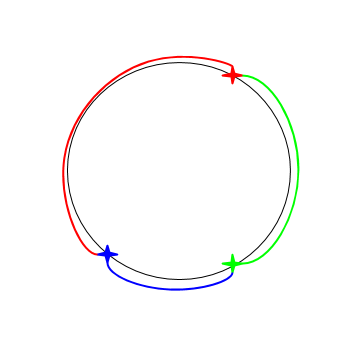
\includegraphics[width=0.5\linewidth]{figs/voro-chord-normal}
	\caption{A Voronoi diagram for a Chord network, using Chord's definition of closest.}
	\label{fig:voro-chord-normal}
\end{figure}

\begin{figure}
	\centering
	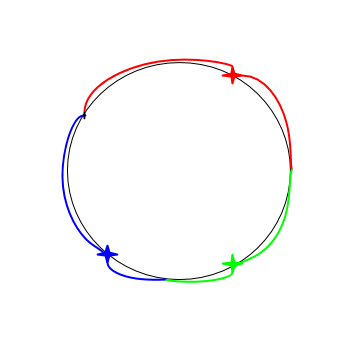
\includegraphics[width=0.5\linewidth]{figs/voro-chord-alternative}
	\caption{A Voronoi diagram for a Chord network, where closest is defined by the node being the closest in either direction.}
	\label{fig:voro-chord-alternative}
\end{figure}

 
\subsection{Terminology}
% % %unified terminology
The large number of DHTs have lead many papers to use different terms to describe congruent elements of DHTs, as some terms may make sense only in one context.
Since this paper will cover multiple DHTs that use different terms, we have created a unified terminology:


\begin{description}
    \item[key] -  The identifier generated by a hash function corresponding to a unique\footnote{Unique with extremely high probability.     The probability of a hash collision is extremely low and are ignored in most formal  specifications for DHTs.  This could be resolved for any file by using any number of the collision resolution strategies, such as chaining or linear probing.  However, resolving a collision of two nodes is much more problematic with no canonical solution other than praying it won't happen.} node or file.
    SHA-1, which generates 160-bit hashes, is typically used as a hashing algorithm.\footnote{Due to the research into hash collisions \cite{stevens2012attacks}, and the glut of hardware that currently exists to perform SHA hash collisions, SHA1 is being depreciated by many companies in 2017. This will undoubtedly lead to some kind of security flaw in a decade or so, when some entrepreneuring hacker figures out a way to force websites to accept a forged SHA1 key.}
    
	\item[ID] - The ID is a key that corresponds to a particular node.  
	The ID of a node and the node itself are referred to interchangeably.
	In this proposal, we refer to nodes by their ID and files by their keys.
	\item[Peer]  - Another active member on the network.
	For this section, we assume that all peers are different pieces of hardware.
	\item[Peerlist] -  The set of all peers that a node knows about. 
	This is sometimes referred to as the \textit{routing table}, but certain DHTs  \cite{pastry} \cite{tapestry}  overload the terminology.
	Any table or list of peers is a subset of the entire peerlist.
	\item[Short-hops] - The subset of peers that are ``closest/adjacent'' to the node in the keyspace, according to the DHT's metric.  
	In a 1-dimensional ring, such a Chord \cite{chord}, this is the node's \textit{predecessor(s)} and \textit{successor(s)}.
	They may also be called \textit{neighbors}.
	\item[Long-hops] - The subset of the peerlist that the node is not adjacent to.  
	These are sometimes referred to as fingers, long links, or shortcuts.
	\item[Root Node] - The node responsible for a particular key. 
	\item[Successor] -  Alternate name for the root node. 
	The successor of a node is the neighbor that will assume a nodes responsibilities if that node leaves. 
    \item[$n$ nodes] -  The number of nodes in the network.
    
\end{description}
Similarly, All DHTs perform the same operations with minor variation.
\begin{description}
	\item[\texttt{lookup(key)}] - This operation finds the root node of \texttt{key}.
	Almost every operation on a DHT needs to leverage the \texttt{lookup} operation in some way.
	\item[\texttt{put(key,value)}] - Stores \texttt{value} at the root node of \texttt{key}.
	Unless otherwise specified, \texttt{key} is assumed be the hashkey of \texttt{value}.
	This assumption is broken in Tapestry.
	\item[\texttt{get(key)}] - This operates like lookup, except the context is to return the value stored by a \texttt{put}.
	This is a subtle difference, since one could \texttt{lookup(key)} and ask the corresponding node directly.
	However, many implementations use backup operations and caching, which will store multiple copies of the value along the network.
	If we do not care which node returns the value mapped with \texttt{key}, or if it is a backup,  we can express it with \texttt{get}.
	\item[\texttt{delete(key, value)}] - This is self-explanatory.  Typically, DHTs do not worry about key deletion and leave that option to the specific application.
    When DHTs do address the issue, they often assume that stored key-value pairs have a specified time-to-live, after which they are automatically removed.
\end{description}

On the local level, each node has to be able to \textit{join }and perform maintenance on itself.
\begin{description}
	\item[\texttt{join()}]  The join process encompasses two steps.
    First, the joining node needs to initialize its peerlist. 
    It does not necessarily need a complete peerlist the moment it joins, but it must initialize one. 
    Second, the joining node needs to inform other nodes of its existence.
    \item[Maintenance]  Maintenance procedures generally are either \textit{active} or \textit{lazy}.
    In active maintenance, peers are periodically pinged and are replaced when they are no longer detected.
    Lazy maintenance assumes that peers in the peerlist are healthy until they prove otherwise, in which case they are either replaced immediately.
    In general, lazy maintenance is used on everything, while active maintenance is only used on neighbors\footnote{check this statement for consistency}.
    
\end{description}

When analyzing the DHTs in this chapter, we look at the overlay's geometry, the peerlist, the \texttt{lookup} function, and how fault-tolerance is performed in the DHTs.
We assume that nodes never politely leave the network but always abruptly fail, since a \texttt{leave()} operation is fairly trivial and has minimal impact.


\section{Chord}
%Chord \cite{chord} is a P2P protocol for file sharing and distributed storage that guarantees a high probability $\log_{2} n$ lookup time for a particular node or file in the network. 
%It is highly fault-tolerant to node failures and churn, the constant joining and leaving of nodes.  It scales extremely well and the network requires little maintenance to handle individual nodes.  



Chord \cite{chord} is the archetypal ring-based DHT and it is impossible to create a new ring-based DHT without making some comparison to Chord.
It is notable due its straightforward routing, its rules which make ownership of keys very easy to sort out, and the large number of derivatives.



% Should I put this in?
Chord is extremely well known in Computer Science, and was awarded the prestigious 2011 SIGCOMM Test of Time Award \cite{zave2012using}.
However, recent research has demonstrated that there have been no correct implementations of Chord in over a decade \cite{zave2012using}.




\subsection*{Peerlist and Geometry}
Chord is a 1-dimensional modular ring in which all messages travel in one direction - upstream, hopping from one node to another node with a greater ID until it wraps around.
Each member of the network and the data stored within it is hashed to a unique $m$-bit key or ID, corresponding to one of the $2^m$ locations on a ring. 
An example Chord network is shown in Figure \ref{fig:chord}.



\begin{figure}
	\centering
	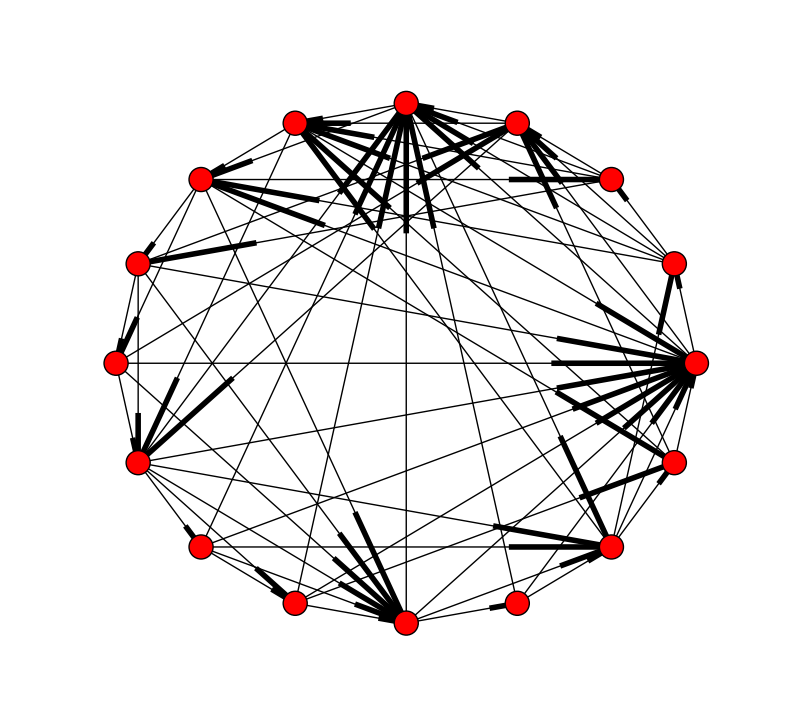
\includegraphics[width=0.45\linewidth]{figs/chord}
	\caption{A Chord ring with 16 nodes.  The fingers (long hop connections) are shown cutting across the ring.}
	\label{fig:chord}
\end{figure}



A node in the network is responsible for all the data with keys upstream from its predecessor's ID, up through and including its own ID.  
If a node is responsible for some key, it is referred to being the root or successor of that key.

Lookup and routing is performed by recursively querying nodes upstream.
Querying only neighbors in this manner would take $O(n)$ time to lookup a key.


To speedup lookups, each node maintains a table of $m$ shortcuts to other peers, called the \textit{finger table}.
The $i$th entry of a node $n$'s finger table corresponds to the node that is the successor of the key $n+2^{i-1} \mod 2^m $.  
During a lookup,  nodes query the finger that is closest to the sought key without going past it, until it is received by the root node.
Each hop essentially cuts the search space for a key in half.
This provides Chord with a highly scalable $\log_2(n)$ lookup time for any key \cite{chord}, with an average $\frac{1}{2}O(\log_{2}(n))$ number of hops.

Besides the finger tables, the peerlist includes a list of $s$ neighbors in each direction for fault tolerance.
This brings the total size of the peerlist to $log_{2}(2^{m})  + 2 \cdot s =  m  + 2 \cdot s$, assuming the entries are distinct.

\subsection*{Joining}
To join the network, node $n$ first asks $n'$ to find \texttt{successor($ n $)}. 
Node $n$ uses the information to set his successor, and maintenance will inform the other nodes of $n$'s existence.
Meanwhile, $n$ will takeover some of the keys that his successor was responsible for.

\subsection*{Fault Tolerance}
Robustness in the network is accomplished by having nodes backup their contents to their $s$ immediate successors, the closest nodes upstream. 
This is done because when a node leaves the or fail, the most immediate successor would be responsible for the keys.
In the case of multiple nodes failing all at once, having a successor list makes it extremely unlikely that any given stored value will be lost.

As nodes enter and leave the ring, the nodes use their maintenance procedures to guide them into the right place and repair any links with failed nodes.  
The process takes $O(\lg^{2}(n))$ messages.
Full details on Chord's maintenance cycle can be found here \cite{chord}.

%\subsection*{Security}
%An Eclipse attack compromises a DHT by poisoning the routing tables of nodes, such that friendly nodes can only communicate with malicious nodes \cite{dhtsec}.
%Because 





\section{Kademlia}
Kademlia \cite{kademlia}  is perhaps the most well known and most widely used DHT, as a modified version of Kademlia (Mainline DHT) is forms backbone of the BitTorrent protocol.
The motivation of Kademlia was to create a way for nodes to incorporate peerlist updates with each query made.

%(the security ramifications of gossip based routing tables being ignored, I suppose).

\subsection*{Peerlist and Geometry}
Like Chord, Kademlia uses $m$-bit keys for nodes and files.
However, Kademlia utilizes a binary tree-based structure, with the nodes acting as the leaves of the tree.
Distance between any two nodes in the tree  is calculated by XORing their IDs.
The XOR distance metric means that distances are symmetric, which is not the case in Chord.

%A node's location in the tree given by the shortest unique prefix of its ID.   
%For each bit in the prefix, there would be a subtree which does not contain that node.  
%Kademlia guarantees that the node will know at least one node in each of these subtrees.

Nodes in Kademlia maintain information about the network using a routing table that contains  $m$ lists, called $k$-buckets.
For each $k$-bucket contains up to $k$ nodes that are distance $2^i$ to $2^{i+1}$, where $0 \leq i < m$.
In other words, each $k$-bucket corresponds to a subtree of the network not containing the node.
An example network is shown in Figure \ref{fig:kademlia}.

\begin{figure}
	\centering
	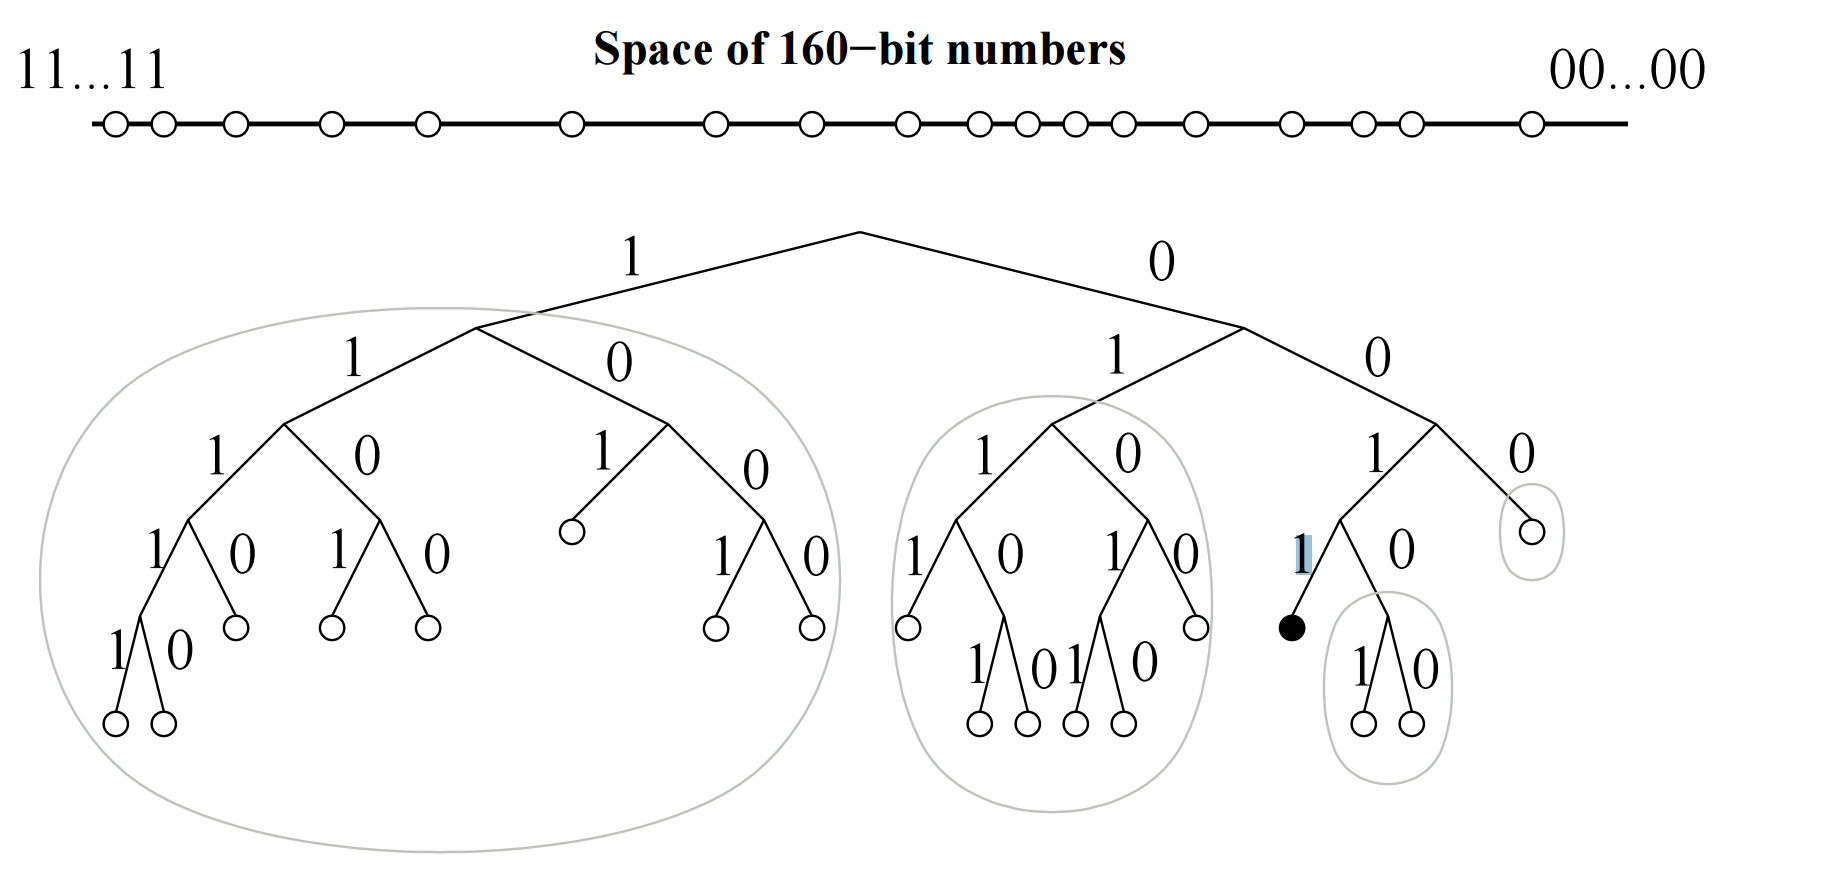
\includegraphics[width=0.7\linewidth]{figs/kademlia}
	\caption{An example Kademlia network from the original paper \cite{kademlia}. The ovals are the node's $k$-buckets.}
	\label{fig:kademlia}
\end{figure}




Each $k$-bucket is maintained by a least recently seen eviction algorithm that skips live nodes.
Whenever the node receives a message, it adds the sender's info to the tail of the corresponding $k$-bucket.
If that info already exists, the info is moved to the tail.

If the $k$-bucket is full, the node starts pinging nodes in the list, starting at the head.
As soon as a node fails to respond, that node is evicted from the list to make way for the new node at the tail.

If there are no modifications to a particular $k$-bucket after a long period of time, the node does a \texttt{refresh} on the $k$-bucket.
A refresh is a \texttt{lookup} of a random key in that $k$-bucket.


%(If I'm an eclipse attacker, I just keep spamming messages of different IDs, but with my own ip address and port info, or with sybils)

\subsection*{Lookup}
In most DHTs, \texttt{lookup(key)} sends a single message and returns the information  of a single node.
The \texttt{lookup} operation in Kademlia differs in both respects:  \texttt{lookup} is done in parallel and each node receiving  a \texttt{lookup(key)} returns the $k$ closest nodes to \texttt{key} it knows about.


A \texttt{lookup(key)} operation begins with the seeking node sending lookups in parallel to the $\alpha$ nodes from the appropriate $k$-bucket.
Each of theses $\alpha$ nodes will asynchronously return the $k$ closest nodes it knows closest to \texttt{key}.
As lookups return their results, the node continue to send lookups until no new nodes\footnote{If a file being stored on the network is the objective, the \texttt{lookup} will also terminate if a node reports having that file.} are found.  

\subsection*{Joining}
A joining node starts with a single contact and then performs a \textit{lookup} operation on its own ID.
Each step of the \textit{lookup} operation yields new nodes for the joining node's peerlist and informs other nodes of its existence.
Finally, the joining node performs a \texttt{refresh} on each $k$-bucket farther away than the closest node it knows of.




\subsection*{Fault-Tolerance}
Nodes actively republish each file stored on the network each hour by rerunning the \texttt{store} command.  
To avoid flooding the network, two optimizations are used.

First if a node receives a \texttt{store} on a file it is holding, it assumes $k-1$ other nodes got that same command and resets the timer for that file.
This means only one node republishes a file each hour.
Secondly, \texttt{lookup} is not performed during a republish.


Additional fault tolerance is provided by the nature of the \texttt{store(data)} operation, which \texttt{puts }the file in the $k$ closest nodes to the key.
However, there is very little in the way of frequent and active maintenance other than what occurs during \texttt{lookup} and the other operations.


%\subsubsection*{Caching}
%Files are cached during a \texttt{get} operation and stored at the closest node that the seeker found that did not return a result.
%The cache has an expiration 










\section{CAN}
%TODO: REREAD, APPARENTLY A COUPLE OF WAYS TO define NEIGHBORHOOD


Unlike the previous DHTs presented in this chapter, the Content Addressable Network (CAN) \cite{can} works in a $d$-dimensional torus, with the entire coordinate space divided among members.
A node is responsible for the keys  that fall within the ``zone'' that it owns.
Each key is hashed into some point within the geometric space.

\subsection*{Peerlist and Geometry}
CAN uses an exceptionally simple peerlist consisting only of neighbors.  
Every node in the CAN network is assigned a geometric region in the coordinate space and each node maintains a routing table consisting each node that borders the node's region.
An example CAN network is shown in Figure \ref{fig:can}


\begin{figure}
	\centering
	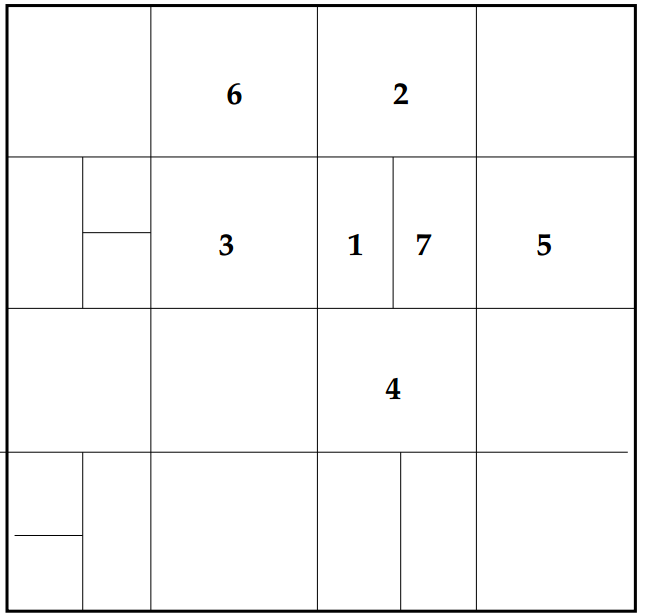
\includegraphics[width=0.7\linewidth]{figs/can}
	\caption{An example CAN network from \cite{can}.}
	\label{fig:can}
\end{figure}


The size of the routing table is a function of the number of dimensions, $O(d)$. 
The lower bound on the routing tables size in a populated network (eg, a network with at least $2d$ nodes) is $\Omega(2d)$.  
This is obtained by looking at each axis, where there is at least one node bordering each end of the axis.
The size of the routing table can grow as more nodes join and the space gets further divided; however, maintenance algorithms prevent the regions from becoming too fragmented.


\subsection*{Lookup}
As previously mentioned, each node maintains a routing table corresponding to their neighbors, those nodes it shares a face with.
Each hop forwards the lookup to the neighbor closest to the destination, until it comes to the responsible node.
In a space that is evenly divided among $n$ nodes, this simple routing scheme uses only $2 \cdot d$ space while giving average path length of $\frac{d}{4}\cdot n^{\frac{1}{d}}$.
The overall lookup time of in CAN is bounded by $O(n^{\frac{1}{d}})$ hops\footnote{Around the same time CAN was being developed, Kleinberg was doing research into small world networks \cite{kleinberg2000small}.  
He proved similar properties for lattice networks with a single shortcut.  What makes this network remarkable is lack of shortcuts.}.

% fault tolerence in routing
If a node encounters a failure during lookup, the node simply chooses the next best path.
However, if lookups occur before a node can recover from damage inflicted by churn, it is possible for the greedy lookup to fail.
The fallback method is to use an expanding ring search until a candidate is found, which recommences greedy forwarding.

\subsection*{Joining}
Joining works by splitting the geometric space between nodes.  
If node $n$ with location $P$ wishes to join the network, it contacts a member of the node to find the node $m$ currently responsible for location $P$.
Node $n$ informs $m$ that it is joining and they divide $m$'s region such that each becomes responsible for half.

Once the new zones have been defined, $n$ and $m$ create its routing table from $m$ and its former neighbors.
These nodes are then informed of the changes that just occurred and update their tables.
As a result, the join operation affects only $O(d)$ nodes.  
More details on this splitting process can be found in CAN's original paper \cite{can}.

\subsection*{Repairing}
A node in a DHT that notifies its neighbors that its leaves usually has minimal impact to the  network and in this is true for most cases in CAN.
A leaving node, $f$, simply hands over its zone to one of its neighbors of the same size, which merges the two zones together.
Minor complications occur if this is not possible, when there is no equally-sized neighbor. 
In this case, $f$ hands its zone to its smallest neighbor, who must wait for this fragmentation to be fixed.



Unplanned failures are also relatively simple to deal with.
Each node broadcasts a heartbeat to its neighbors, containing its and its neighbors' coordinates.
If a node fails to hear a heartbeat from $f$ after a number of cycles, it assumes $f$ must have failed and begins a \texttt{takeover} countdown.
When this countdown ends, the node broadcasts\footnote{This message is sent to all of $f$'s neighbors.} a \texttt{takeover} message in an attempt to claim $f$'s space.
This message contains the node's volume.
When a node receives a \texttt{takeover} message, it either cancels the countdown or, if the node's zone is smaller than the broadcaster's, responds with its own \texttt{takeover}.

The general rule of thumb for node failures in CAN is that the neighbor with the smallest zone takes over the zone of the failed node.
This rule leads to quick recoveries that affect only $O(d)$ nodes, but requires a zone reassignment algorithm to remove the fragmentation that occurs from \texttt{takeovers}.

To summarize, a failed node is detected almost immediately, and recovery occurs extremely quickly, but fragmentation must be fixed by a maintenance algorithm.




%As mentioned earlier in the text, Ratnasamy et al. \cite{can}  also present the concept own using landmarks to choose coordinates, rather than a has function.
%Each node measures the round-trip time (RTT) to each to of the $m$ landmarks, which yields one of $m!$ permutations.
%The keyspace is partitioned into $m!$ regions, each corresponding to one of the orderings.  
%A joining node now chooses a random location from the region corresponding to its landmark ordering.






%\subsection*{Design Improvements}
%Ratnasamy et al.\ identified a number of improvements that could be made to CAN \cite{can}.
%Some of these improvements have already be explored in Chapter 1.

%One modification to the system is increasing the number of dimensions in the coordinate space.
%Increasing $d$ improves fault tolerance and reduces path length.

%One concept Ratnasamy et al.\  introduces is the idea of multiple coordinate spaces existing simultaneously, called \textit{realities}. 
%Each object in the DHT exists at a different set of coordinates for each reality simultaneously.
%So a node might have coordinates $(x_0,y_0,z_0)$ in one reality, while having coordinates $(x_1,y_1,z_1)$ in another.
%Independent sets of neighbors for each reality yield different the overall topologies and mappings of keys to nodes.
%Multiple realities increase the cost of maintenance and routing table sizes, but provide greater fault tolerance and greater data availability.

%A final modification is to allow multiple nodes shares the same zone (ie zones don't necessarily split as a result of a join operation).    


\section{Pastry}

%Addressing - 128 bit ID, 0 to $2^{128} -1$, assigned randomly using hash.   but thought of as base $2^{b}$ numbers (typically b=4).  
Pastry \cite{pastry} and Tapestry \cite{tapestry} are extremely similar use a prefix-based routing mechnism introduced by Plaxton et al.\ \cite{plaxton1999accessing}.
In Pastry and Tapestry, each key is encoded as a base $ 2^{b} $ number (typically $b=4$ in Pastry, which yields easily readable hexadecimal).
The resulting peerlist best resembles a hypercube topology \cite{induced}, with each node being a vertice of the hypercube.

One notable feature of Pastry is the incorperation of a proximity metric.
The peerlist uses IDs that are close to the node according to this metric.

\subsection*{Peerlist}
Pastry's peerlist consists of three components: the routing table, a leaf set, and a neighborhood set.  
The routing table consists of $\log_{2^{b}}(n)$ rows with $2^{b} -1 $ entries per row. 
The $i$th level of the routing table correspond to the peers with that match first $i$ digits of the example nodes ID.

Thus, the 0th row contains peers which don't share a common prefix with the node, the 1st row contains those that share a length 1 common prefix, the 2nd a length 2 common prefix, etc.  
Since each ID is a base $2^b$ number, there is one entry for each of the $2^{b} -1 $ possible differences.   

For example, let is consider a node 05AF in system where $b = 4$ and the hexadecimal keyspace ranges from $0000$ to FFFF.
\begin{itemize}
    \item 1322 would be an appropriate peer for the 1st entry of level 0.
    \item 0AF2 would be an appropriate peer for the 10th\footnote{0 is the 0th level.} entry of level 1.
    \item 09AA would be an appropriate peer for the 9th entry of level 1.	
    \item 05F2 would be an appropriate peer for the 2nd entry of level 3.
\end{itemize}


The leaf set is used to hold the $L$ nodes with the numerically closest IDs;  half of it for smaller IDs and half for the larger.
A typical value for $L$ is $2^b$ or $2^{b+1}$.
The leaf set is used for routing when the destination key is close to the current node's ID.
The neighborhood set contains the $L$ closest nodes, as defined by some proximity metric.  
It, however, is generally not used for routing.  
Figure \ref{fig:pastry-table} shows an example peerlist of a node in PAST.

\begin{figure}
	\centering
	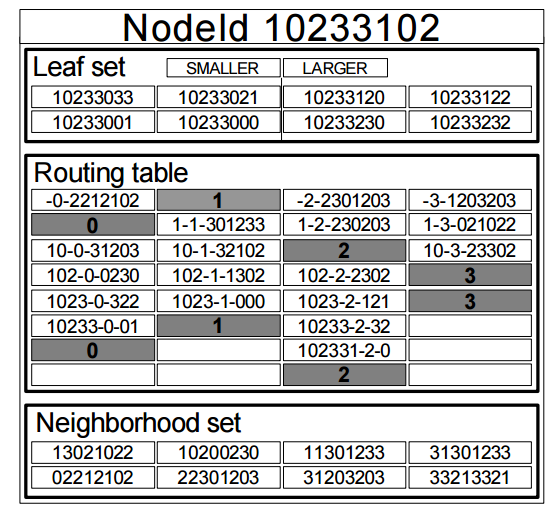
\includegraphics[width=0.5\linewidth]{figs/pastry-table}
	\caption{An example peerlist for a node in Pastry \cite{pastry}.}
	\label{fig:pastry-table}
\end{figure}



\subsection*{Lookup}
The \texttt{lookup} operation is a fairly straightforward recursive operation.
The \texttt{lookup(key)} terminates when the \texttt{key} is falls within the range of the leaf set, which are the nodes \emph{numerically} closest to the current node.
In this case, the destination will be one of the leaf set, or the current node.

If the destination node is not immediately apparent, the node uses its routing table to select the next node.
The node looks at the length $l$ shared prefix,  at examines the $l$th row of its routing table.
From this row, the \texttt{lookup} continues with the entry that matches at least another digit of the prefix.
In the case that this entry does not exist or has failed, the \texttt{lookup} continues from the closest ID chosen from the entire peerlist.
This process is described by Algorithm \ref{PastryLookup}.
Lookup is expected  to take $\lceil \log_{2^{b}} \rceil $, as each hop along the routing table reduces the search space by $\frac{1}{2^{b}}$.
 
\begin{algorithm}
    \caption{Pastry lookup algorithm}
    \label{PastryLookup}
    \begin{algorithmic}
        \State Let $L$ be the routing  
        \Function{Lookup}{$key$}
            \If {$key$ is in the range of the leaf set }
            	\State destination is closest ID in the leaf set or self
            \Else
            	\State $next\gets$ entry from routing table that matches $\geq 1$ more digit
            	\If {$next \neq null$}
                	\State forward to $next$
            	\Else
                	\State forward to the closest ID from the entire peerlist
                \EndIf
                
            \EndIf
        \EndFunction
    \end{algorithmic}
\end{algorithm}

\subsection*{Joining}
To join the network, node $J$ sends a \texttt{join} message to $A$, some node that is close according to the proximity metric.
The \texttt{join} message is forwarded along like a \texttt{lookup} to the root of $X$, which we'll call $root$.
Each node that received the \texttt{join} sends a copy of the their peerlist to $J$.

The leaf set is constructed from copying $root$'s leaf set, while $i$th row in the routing table routing table is copied from the $i$th node contacted along the \texttt{join}.
The neighborhood set is copied from $A$'s neighborhood set, as \texttt{join} predicates that $A$ be close to $J$.
This means $A$'s neighborhood set would be close to $A$. 

After the joining node creates its peerlist, it sends a copy to each node in the table, who then can update their routing tables.  
The cost of a \texttt{join} is $O(log_{2}^{b} n)$ messages,  with  a constant  coefficient  of $3*2^{b}$




\subsection*{Fault Tolerance}
Pastry lazily repairs its leaf set and routing table.
When node from the leaf set fails, the node contacts the node with largest or smallest ID (depending if the failed node ID was smaller or larger respectively) in the leaf set.
That node returns a copy of its leaf set, and the node replaces the failed entry.
If the failed node is in the routing table, the node contacts a node with an entry in the same row as the failed node for a replacement.

Members of the neighborhood set are actively checked.
If a member of the neighborhood set is unresponsive, the node obtains a copy of another entry's neighborhood set and repairs from a selection.



%\subsection*{Proximity Metric}
%Pastry's goal is to minimize the ``distance'' messages travel, where distance can be defined by some metric, typically the number of hops.
%The leaf set is the  of nodes closest to the node in the keyspace.  
%The neighborhood set is the of nodes closest to the node according to the distance metric. 
%Guarantees routing time is  $<\log n$ in typical operation.  
%Guarantees eventual delivery except when half of the leaf nodes fail simultaneously.






%\section{Tapestry}
%Tapestry \cite{tapestry} is based off the same prefix-based lookup \cite{prr} as Pastry \cite{pastry} and the peerlist and lookup operation share many similarities.
%Tapestry views itself more as a DOLR \cite{dolr}.
%This essentially means that it is a distributed key-based lookup system like a DHT \cite{hildrum2004distributed}, but with some subtle differences at the abstract level which manifest as large %implementation changes.
%The essential difference here is that Tapestry has servers \textit{publish} records/objects on the network, which direct lookups to the server.  
%The assumption here seems to be that the servers, not the responsible node, serve the actual data.  
%DHTs care or don't care on an application to application basis whether keys are associated with records or content. 






% ``Small'' routing tables
\section{Symphony and Small World Routing}
Symphony  \cite{symphony} is a 1$d$ ring-based DHT similar to Chord \cite{chord}, but is constructed using the properties of small world networks \cite{kleinberg2000small}.
Small world networks owe their name to a phenomena observed by psychologists in the late 1960's. 

Subjects in experiments were to route a postal message to a target person; for example the wife of a Cambridge divinity student in one experiment and a Boston stockbroker in another \cite{milgram1967small}.
The messages were only to be routed by forwarding them to a friend they thought most likely to know the target.
Of the messages that successfully made their way to the destination, the average path length from a subject to a participant was only 5 hops.  

This lead to research investigating creating a network with randomly distributed links, but with a efficient lookup time.
Kleinberg \cite{kleinberg2000navigation} showed that in a 2-dimensional lattice network, nodes could route messages in $O(\log^{2}n)$ hops using only their neighbors and a single randomly chosen\footnote{Randomly chosen from a specified distribution.} finger.
In other words, $O(\log^{2}n)$ lookup is achievable with a $O(1)$ sized routing table.

\subsection*{Peerlist}
Rather than the 2-dimensional lattice used by Kleinberg, Symphony uses a 1-dimensional ring\footnote{This is technically a 1-dimensional lattice.} like Chord.
Symphony assigns $m$-bit keys to the modular unit interval $ [0,1)$, instead of using a keyspace ranging from 0 to $2^{n} - 1$.
This location is found  with $\frac{hashkey}{2^{m}}$.
This is arbitrary from a design standpoint, but makes choosing from a random distribution simpler. 

Nodes know both their immediate predecessor and successor, much like in Chord.
Nodes also keep track of some  $k \geq 1$ fingers, but, unlike in Chord, these fingers are chosen at random.
These fingers are chosen from a probability distribution corresponding to the expression $e^{ln(n) + (rand48() - 1.0)}$, where $n$ is the number of nodes in the network and \texttt{rand48()} is a C function that generates a random float?double between 0.0 and 1.0.
Because $n$ os difficult to compute due to the changing nature of P2P networks, each node uses an approximation is used based on the distance between themselves and their neighbors.

A final feature of note is that links in Symphony are bidirectional.
Thus, if a node creates a finger to a peer, that peer creates a, so nodes in Symphony have a grand total of $2k$ fingers.
%(although it gets me thinking, is there any advantage/statistical properties   that could be exploited by making the space monic)


\subsection*{Joining and Fault Tolerance}
The joining and fault tolerance processes in Symphony are extremely straightforward.
After determining its ID, a joining node asks a member to find the root node for its ID.
The joining node integrates itself in between its predecessor and successor and then randomly generates its fingers.

Failures of immediate neighbors are handled by use of successor and predecessor lists
Failures for fingers are handled lazily and are replaced by another randomly generated link when a failure is detected.

% Large Routing Tables
\section{ZHT}
One of the major assumptions of DHT design is that churn is a significant factor, which requires constant maintenance to handle.
A consequence of this assumption is that nodes only store a small subset of the entire network to route to.
Storing the entire network is not scalable for the vast majority of distributed systems due to bandwidth constraints and communication overhead incurred by the constant joining and leaving of nodes.

In a system that does not expect churn, the memory and bandwidth costs for each node to keep a full copy of the routing table are minimal.
An example of this would be a data center or a cluster built for higher-performance computing, where churn would overwhelmingly be the result of hardware failure, rather than users quitting.

ZHT \cite{li2013zht} is an example of such a system, as is Amazon's Dynamo \cite{dynamo}.
ZHT is a ``zero-hop hash table,'' which takes advantage of the fact that  nodes in  High-End Computing environments have a predictable lifetime.
Nodes are created when a job begins and are removed when a job ends.
This property allows ZHT to \texttt{lookup} in $ O(1) $ time.

\subsection*{Peerlist}

ZHT operates in a 64-bit ring, for a total of $N = 2^{64}$ addresses.
ZHT places a  hard limit of $ n $ on the maximum number of physical nodes in the network, which means the network has $n$ partitions of $\frac{N}{n} =  \frac{2^{64}}{n}$ keys.
The partitions are evenly divided along the network.

The network consists of $k$ physical nodes which each are running at least one instance (virtual nodes) of ZHT, with a combined total of $i$ .
Each instance is responsible for some span of partitions in the ring.


Each node maintains a complete list of all nodes in the network, which do not have to be updated very often due to the lack of or very low levels of churn.
The memory cost is extremely low.
Each instance has a 10MB footprint, and each entry for the membership table takes only 32 bytes per node.
This means routing takes anywhere between 0 to 2 hops (explained below).

\subsection*{Joining}
ZHT operates under a static or dynamic membership.
In a static membership, no nodes will be joining the network once the network has been bootstrapped.
Nodes can join at any time when ZHT is using dynamic membership.

To join, the joiner asks a random member for a copy of the peerlist 
The joiner can then determine which node is the most heavily overloaded.
The joiner chooses an address in the network to take over partitions from that node.

\subsection*{Fault Tolerance}
Fault tolerance exists to handle only hardware failure or planned departures from the network.
Nodes backup their data to their neighbors.

\section{Summary}
% % % table
% Perhaps geometries should be included?
% be sure to include join and leave costs.

We have seen that there are a wide variety of distributed hash tables, but they have some clearly defined characteristics that bind them all together.
Table \ref{tab:tradeoffs} summarizes the information presented in this chapter.


\begin{table}[h]
	\tiny
	\centering
	\begin{tabularx}{\textwidth}{ |X|X|X|X|X| }
		\hline
		% Add join leave cost, avgerages and maxs
		DHT & Routing Table Size & Lookup Time & Join/Leave & Comments \\ \hline  
		
		Chord \cite{chord} & $O(\log n)$, maximum $m +2s$ & $O(\log n)$, avg $(\frac{1}{2} \log n)$  &  $<O(\log n^{2})$ total messages& $m$  = keysize in bits, $s$ is neighbors in 1 direction  \\ \hline
		
		Kademlia \cite{kademlia} & $O(\log n)$, maximum $m\ \cdot k$ & $(\lceil \log n\rceil) + c$ & $O(\log(n))$& This is without considering optimization   \\ \hline
		CAN \cite{can} & $\Omega(2d)$ & $O(n^{\frac{1}{d}})$, average $\frac{d}{4}\cdot n^{\frac{1}{d}}$ & Affects $O(d)$ nodes & $d$ is the number of dimensions \\ \hline
		
		Plaxton-based DHTs, Pastry \cite{pastry}, Tapestry \cite{tapestry} & $O(\log_{\beta} n)$ & $ O(\lceil \log_{2^{\beta}} \rceil) $ & $O(\log_{\beta} n)$ &  NodeIDs are base $\beta$ numbers \\ \hline
		
        Symphony \cite{symphony}& $2k + 2$&   average $O(\frac{1}{k} \log^{2} n )$ & $O(\log^{2} n)$ messages,  constant $<1$ &  $k \geq 1$, fingers are chosen at random\\ \hline  
		
        ZHT \cite{li2013zht}&   $O(n)$& $O(1)$ &  $O(n)$ & Assumes an extremely low churn \\ \hline
        
        VHash & $\Omega(3d+1) + O((3d+1)^{2})$ & $O(\sqrt[d]{n})$ hops & $3d + 1$ & approximates regions, hops are based least latency\\ \hline
	\end{tabularx}
	\caption{The different ratios and their associated DHTs}
	\label{tab:tradeoffs}
\end{table}

% % % Specific DHTs



 %done
	\chapter{ChordReduce}
\label{chapter:chordreduce}

As we have previously discussed, Google's MapReduce \cite{mapreduce} paradigm has rapidly become an integral part in the world of data processing and is capable of efficiently executing numerous Big Data programming and data-reduction tasks.  
The paradigm MapReduce is much simpler than the previous sentence suggests.
By using MapReduce, a user can take a large problem, split it into small, equivalent tasks and send those tasks to other processors for computation.  
The results are sent back to the user and combined into one answer.  

Many popular platforms for MapReduce, such as Hadoop \cite{hadoop}, utilize a central source of coordination and organization to store and operate on data.
The hierarchical structure of Hadoop results in a single point of failure at the node that concentrates the results and also requires a complicated scheme for handling node failures.

We developed a system, called ChordReduce, which was our first attempt to leverage the qualities of a DHT to create a distributed computing platform.  
It is a system that can scale, is fault tolerant, has a minimal amount of latency, and distributes tasks evenly.  
ChordReduce leverages the underlying protocol from Chord \cite{chord} to distribute Map and Reduce tasks to nodes evenly, provide greater data redundancy, and guarantee a greater amount of fault tolerance. 
Rather than viewing Chord solely as a means for sharing files, we see it as a means for distributing work. This paper establishes the effectiveness of using Chord as a framework for distributed programming. At the same time we avoid the architectural and file system constraints of systems like Hadoop.  


\section{Background}
ChordReduce takes its name from the two components it is built upon.
Chord \cite{chord} provides the backbone for the network and the file system, providing scalable routing, distributed storage, and fault-tolerance.   
MapReduce runs on top of the Chord network and utilizes the underlying features of the distributed hash table.  This section provides an extensive and expanded background on Chord and MapReduce.


\subsection{Chord}
Chord \cite{chord} is a P2P protocol for file sharing that uses a hash function to assign addresses to nodes and files for a ring overlay. The Chord protocol takes in some key and returns the identity (ID) of the node responsible for that key.  These keys are generated by hashing a value of the node, such as the IP address and port, or by hashing the filename of a file.  The hashing process creates a $m$-bit hash identifier.

The nodes are then arranged in a ring from the lowest hash-value to highest.  Chord takes the files and places each in the node that has the same hashed identifier as it.  If no such node exists, the node with the first identifier that follows this value is selected. Since the overlay is a circle, this assignment is computed in modulo $2^m$ space.  

The node responsible for the key $\kappa$ is called the $successor$ of $\kappa$, or $successor(\kappa)$.  For example, if there were some portion of the network with nodes 20, 25, and 27, node 25 would be responsible for the files with the keys (21,22,23,24,25). If node 25 were to decide to leave the network, its absence would be detected by node 27, who would then be responsible for all the keys node 25 was covering, in addition to its own keys. 
\begin{figure}
	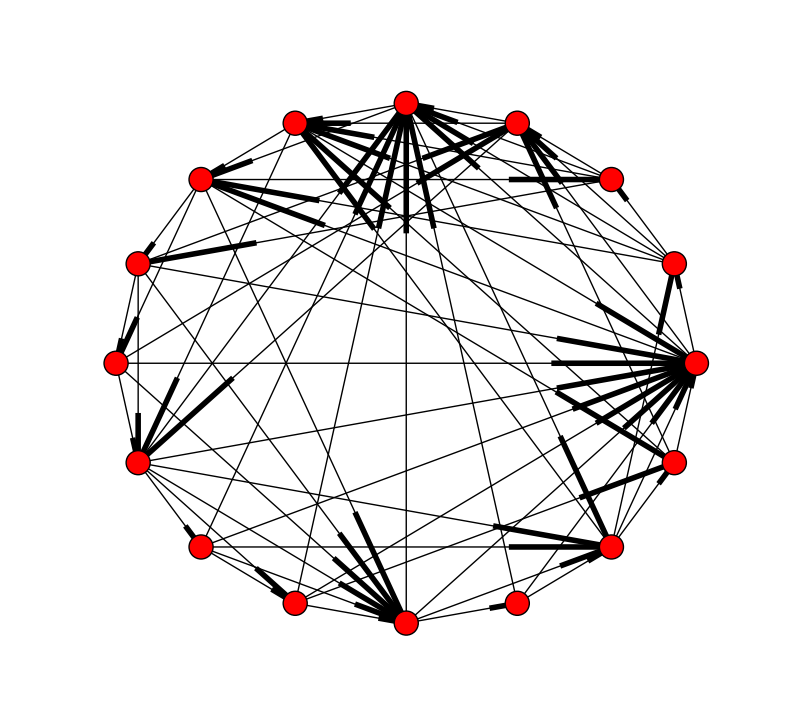
\includegraphics[width=\linewidth]{figs/chordreal}
	\caption{A Chord ring with 16 nodes.  The bold lines are incoming edges.  Each node has a connection to its successor, as well as 4 fingers, some of which are duplicates.}
	\label{fig:chordreal}
\end{figure}


With this scheme, we can reliably find the node responsible for some key by asking the next node in the circle for the information, who would then pass the request through the circle until the successor was found.  We can then proceed to directly connect with the successor to retrieve the file.  This naive approach is largely inefficient, and is a simplification of the lookup process, but it is the basis of how Chord theoretically works.

To speed up the lookup time, each node builds and maintains a \emph{finger table}.  The \emph{finger table} contains the locations of up to $m$ other nodes in the ring.  The $i$th entry of node $n$'s \emph{finger table} corresponds to the node that is the $successor(n+2^{i-1})$ $mod$ $2^m$. Hash values are not perfectly distributed, it is possible to have duplicate entries in the \emph{finger table}. An example Chord network with fingers is shown in in Fig. \ref{chordreal}.


\begin{figure}
	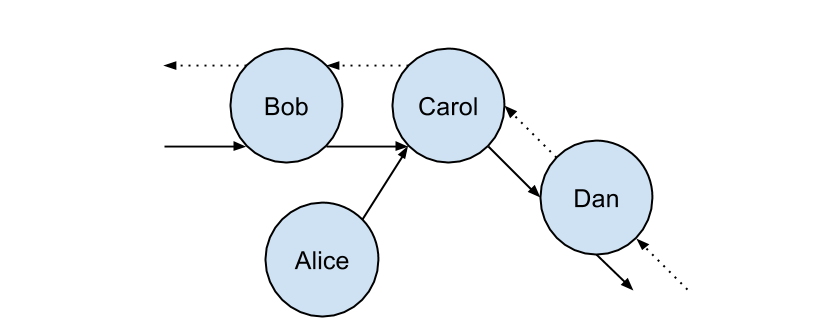
\includegraphics[width=\linewidth]{figs/abcd1}
	\caption{Alice has incorrectly determined that Carol is her appropriate successor.  When Alice stabilizes, Carol will let her know about Bob.}
	\label{fig:abcd1}
\end{figure}


\begin{figure}
	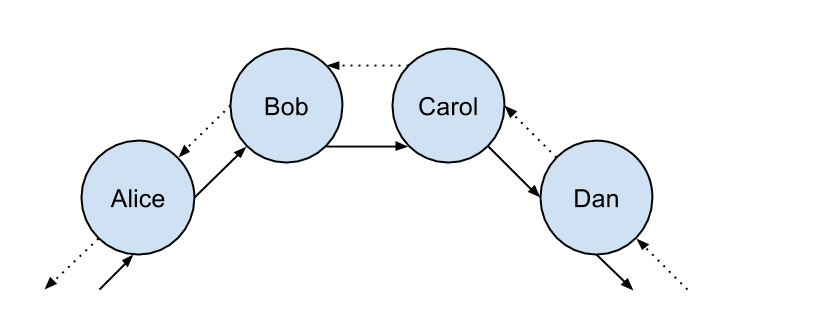
\includegraphics[width=\linewidth]{figs/abcd2}
	\caption{After completing stabilize, Alice makes Bob her successor and notifies him. Bob then made Alice as his predecessor.}
	\label{fig:abcd2}
\end{figure}



When a node $n$ is told to find some key, $n$ looks to see if the key is between $n$ and $successor(n)$ and return $successor(n)$'s information to the requester. If not, it looks for the entry in the finger table for the closest preceding node $n'$ it knows and asks $n'$ to find the successor.  This allows each step to skip up to half the nodes in the network, giving a $\log_2(n)$ lookup time.  Because nodes can constantly join and leave the network, each entry in the table is periodically checked and updated during a finger maintenance period. 

To join the network, node $n$ first asks $n'$ to find $successor(n)$ for it.  Node $n$ uses the information to set his successor, but the other nodes in the ring will not acknowledge $n$'s presence yet.  Node $n$ relies on the stabilize routine to fully integrate into the ring.

The stabilize routine helps the network integrate new nodes and route around nodes who have left the network. Each node periodically checks to see who their successor's predecessor is.  In the case of a static network, this would be the checking node.  However, if the checking node gets back a different node, it looks at that returned node's hash value and changes its own successor if needed.  Regardless of whether the checking node changes its successor, that node then notifies the (possibly) new successor,  who then checks if he needs to change his predecessor based on this new information.  While complex, the stabilization process is no more expensive than a heartbeat function.  A more concrete example:


Suppose Alice, Bob, Carol, and Dan are members of the ring and everyone is ordered alphabetically (Fig. \ref{fig:abcd1}). Alice is quite sure that Carol is her successor.  Alice asks Carol who her predecessor is and Carol says Bob is.  Since Bob is closer than Carol, Alice changes her successor to Bob and notifies him.  

When Bob sees that notification, he can see Alice is closer than whoever his previous predecessor is and sets Alice to be his predecessor.  During the next stabilization cycle, Alice will see that she is still Bob's predecessor and notify him that she's still there (Fig. \ref{fig:abcd2}).

To prevent loss of data due to churn, each node sends a backup of their data to their successor.  Section IV discusses the implementation of the backup process in ChordReduce and expands upon it for backing up Map and Reduce tasks.


\subsection{Extensions of Chord}

The Cooperative File System (CFS) is an anonymous, distributed file sharing system built on top of Chord \cite{CFS}.  In CFS, rather than storing an entire file at a single node, the file is split up into multiple chunks around 10 kilbytes in size.  These chunks are each assigned a hash and stored in nodes corresponding to their hash in the same way that whole files are.  The node that would normally store the whole file instead stores a \emph{key block}, which holds the hash address of the chunks of the file. 

The chunking allows for numerous advantages.  First, it promotes load balancing. Each piece of the overall file would (ideally) be stored in a different node, each with a different backup or backups.  This would prevent any single node from becoming overwhelmed from fulfilling multiple requests for a large file.  It would also prevent retrieval from being bottlenecked by a node with a relatively low bandwidth. Finally, when Chord uses some sort of caching scheme like that described in CFS \cite{CFS}, caching chunks as opposed to the entire file resulted in about 1000 times less storage overhead.  

Mutable files  and IRM, which is short for Integrated File Replication and Consistency Maintenance \cite{irm}, has nodes keep track of file requests they initiate or forward.  If they find they are frequently forwarding a request for a particular file, they store that file locally until it is no longer requested frequently.  What makes IRM unique is that it combines caching with a 

Chunking also opens up the options for implementing additional redundancy such as erasure codes \cite{rizzo1997effective}. With erasure codes, redundant chunks are created but any combination of a particular number of chunks is sufficient to recreate the file.  For example, a file that would normally be split into 10 chunks might be split into 15 encoded chunks.  The retrieval of any 10 of those 15 chunks is enough to recreate the file.  Implementing erasure codes would presumably make the network more fault tolerant, but that is an exercise left for future work.


Generally, related files should be kept together; Chord, however, just hashes the filename to find the responsible node and sends it to that location without any thought to organization.  Our solution to this is to use allow the file owner to select first 80 bits of a file's hash, then generating the remaining least signifcant bits by hashing the filename.  It does not matter if a file owner, in some infinitesimally small coincidence, chooses the same 80 bit prefix as another file owner, as the purpose is to keep related files together.    % done
	\chapter{VHash And DGVH}
DHTs all seek to minimize lookup time for their respective topologies.
This is done by minimizing the number of overlay hops needed for a lookup operation.
This is a good approximation for minimizing the latency of lookups, but does not actually do so, as each hop has a different amount of latency.
Furthermore, a network might need to minimize some arbitrary metric, such as energy consumption.

VHash is a multi-dimensional DHT that minimizes routing over some given metric.
It uses a fast approximation of a Delaunay Triangulation to compute the Voronoi tessilation of a multi-dimensional space.
%Approximated routing tables



Arguably all Distributed Hash Tables (DHTs) are built on the concept of Voronoi tessellations.
In all DHTs, a node is responsible for all points in the overlay to which it is the ``closest'' node.
Nodes are assigned a key as their location in some keyspace, based on the hash of certain attributes.
Normally, this is just the hash of the IP address (and possibly the port) of the node \cite{chord} \cite{kademlia} \cite{can} \cite{pastry}, but other metrics such as geographic location can be used as well \cite{ratnasamy2002ght}.

These DHTs have carefully chosen metric spaces such that these regions are very simple to calculate.
For example, Chord \cite{chord} and similar ring-based DHTs \cite{symphony} utilize a unidirectional, one-dimensional ring as their metric space, such that the region for which a node is responsible is the region between itself and its predecessor.

Using a Voronoi tessellation in a DHT generalizes this design.
Nodes are Voronoi generators at a position based on their hashed keys.
These nodes are responsible for any key that falls within its generated Voronoi region.

Messages get routed along links to neighboring nodes.
This would take $O(n)$ hops in one dimension.
In multiple dimensions, our routing algorithm (Algorithm \ref{alg:lookup}) is extremely similar to the one used in Ratnasamy et al.'s Content Addressable Network (CAN) \cite{can}, which would be $O(n^{\frac{1}{d}})$ hops.


\begin{algorithm}
	\caption{Lookup in a Voronoi-based DHT}
	\label{alg:lookup}
	\begin{algorithmic}[1]
		\State Given node $n$
		\State Given $m$ is a message addressed for $loc$
		\State $potential\_dests \leftarrow n \cup n.short\_peers \cup n.long\_peers$
		\State $c \leftarrow $ node in $ potential\_dests$ with shortest distance to $loc$
		\If{$c$ == $n$}
			\State \Return $n$
		\Else
			\State \Return $c.lookup(loc)$
		\EndIf
	\end{algorithmic}
\end{algorithm}


Efficient solutions, such as Fortune's sweepline algorithm \cite{fortune1987sweepline}, are not usable in spaces with 2 more dimensions.
As far as we can tell, there is no way efficient to generate higher dimension Voronoi tessellations, especially in the distributed Churn-heavy context of a DHT.
Our solution is the Distributed Greedy Voronoi Heuristic.

\section{Distributed Greedy Voronoi Heuristic}
A Voronoi tessellation is the partition of a space into cells or regions along a set of objects $O$, such that all the points in a particular region are closer to one object than any other object.
We refer to the region owned by an object as that object's Voronoi region.
Objects which are used to create the regions are called Voronoi generators.
In network applications that use Voronoi tessellations, nodes in the network act as the Voronoi generators.

The Voronoi tessellation and Delaunay triangulation are dual problems, as an edge between two objects in a Delaunay triangulation exists if and only if those object's Voronoi regions border each other.
This means that solving either problem will yield the solution to both.
An example Voronoi diagram is shown in Figure \ref{voro-ex}.
For additional information, Aurenhammer \cite{voronoi} provides a formal and extremely thorough description of Voronoi tessellations, as well as their applications.


\begin{figure}
	\centering
	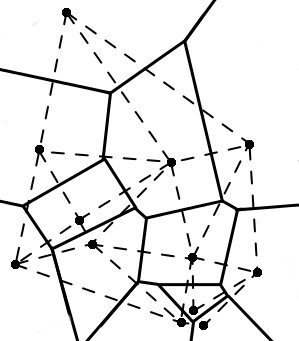
\includegraphics[width=0.5\linewidth]{figs/voronoi}
	\caption{An example Voronoi diagram for objects on a 2-dimensional space.  The black lines correspond to the borders of the Voronoi region, while the dashed lines correspond to the edges of the Delaunay Triangulation.}
	\label{voro-ex}
\end{figure}




The Distributed Greedy Voronoi Heuristic (DGVH) is a fast method for nodes to define their individual Voronoi region (Algorithm \ref{alg:dgvh}).
This is done by selecting the nearby nodes that would correspond to the points connected to it by a Delaunay triangulation.
The rationale for this heuristic is that, in the majority of cases, the midpoint between two nodes falls on the common boundary of their Voronoi regions.

%In addition, nodes should only have to compute their own Voronoi region, and possibly estimate those of its neighbors.
%Anything else is a waste of processing power.



\begin{algorithm} % make smaller
	\caption{Distributed Greedy Voronoi Heuristic}
	\label{alg:dgvh}
	\begin{algorithmic}[1]  % the numberis how many lines
		\State Given node $n$ and its list of $candidates$.
		\State Given the minimum $table\_size$
		\State $short\_peers \leftarrow$ empty set that will contain $n$'s one-hop peers
		\State $long\_peers \leftarrow$ empty set that will contain $n$'s two-hop peers
		\State Sort $candidates$ in ascending order by each node's distance to $n$
		\State Remove the first member of $candidates$ and add it to $short\_peers$
		\ForAll{$c$ in $candidates$}
		\State $m$ is the midpoint between $n$ and $c$
		\If{Any node in $short\_peers$ is closer to $m$ than $n$}
		\State Reject $c$ as a peer
		\Else
		\State Remove $c$ from $candidates$
		\State Add $c$ to $short\_peers$
		\EndIf
		\EndFor
		\While{$|short\_peers| < table\_size$ \textbf{and} $|candidates| >0$}
		\State Remove the first entry $c$ from $candidates$
		\State Add $c$ to $short\_peers$
		\EndWhile
		\State Add $candidates$ to the set of $long\_peers$
		\If{$|long\_peers| > table\_size^2$}
		\State $long\_peers \leftarrow$ random subset of $long\_peers$ of size $table\_size^2$
		\EndIf
	\end{algorithmic}
\end{algorithm}


During each cycle, nodes exchange their peer lists with a current neighbor and then recalculate their neighbors.
A node combines their neighbor's peer list with its own to create a list of candidate neighbors.
This combined list is sorted from closest to furthest.
A new peer list is then created starting with the closest candidate.
The node then examines each of the remaining candidates in the sorted list and calculates the midpoint between the node and the candidate.
If any of the nodes in the new peer list are closer to the midpoint than the candidate, the candidate is set aside.
Otherwise the candidate is added to the new peer list.


DGVH never actually solves for the actual polytopes that describe a node's Voronoi region.
This is unnecessary and prohibitively expensive \cite{raynet}.
Rather, once the heuristic has been run, nodes can determine whether a given point would fall in its region.

Nodes do this by calculating the distance of the given point to itself and other nodes it knows about.
The point falls into a particular node's Voronoi region if it is the node to which it has the shortest distance.
This process continues recursively until a node determines that itself to be the closest node to the point.
Thus, a node defines its Voronoi region by keeping a list of the peers that bound it.



\subsection{Algorithm Analysis}

DVGH is very efficient in terms of both space and time.
Suppose a node $n$ is creating its short peer list from $k$ candidates in an overlay network of $N$ nodes.
The candidates must be sorted, which takes $O(k\cdot\lg(k))$ operations.
Node $n$ must then compute the midpoint between itself and each of the $k$ candidates.
Node $n$ then compares distances to the midpoints between itself and all the candidates.
This results in a cost of

\[ k\cdot\lg(k) + k \text{ midpoints}  + k^{2} \text{ distances} \]


Since $k$ is  bounded by $\Theta(\frac{\log N}{\log \log N} )$ \cite{bern1991expected} (the expected maximum degree of a node), we can translate the above to

\[O(\frac{\log^{2} N}{\log^{2} \log N} )\]

In the vast majority of cases, the number of peers is equal to the minimum size of \textit{Short Peers}.
This yields $k=(3d+1)^{2}+3d+1$ in the expected case, where the lower bound and expected complexities are $\Omega(1)$.



\section{Experimental Results}
We evaluated the effectiveness of VHash and DGVH in creating a set of experiments.\footnote{Our results are pulled directly from \cite{dgvh} and \cite{vhash}.}
The first experiment showed how VHash could use DGVH to create a routing mesh.
Our second showed how optimizing for latency yielded better results than optimizing for least hops.

\subsection{Convergence}
Our first experiment examined how DGVH could be used to create a routing overlay and how well it performed in this task.
The simulation demonstrated how DGVH  formed a stable overlay from a chaotic starting topology after a number of cycles.
We compared our results to those in RayNet \cite{raynet}.
The authors of Raynet proposed a random $k$-connected graph would be a challenging initial configuration for showing a DHT relying on a gossip mechanism could converge to a stable topology.

In the initial two cycles of the simulation, each node bootstrapped its short peer list by appending 10 nodes, selected uniformly at random from the entire network.
In each cycle, the nodes gossiped , swapping peer list information.
They then ran DGVH using the new information.
We calculated the hit rate of successful lookups by simulating 2000 lookups from random nodes to random locations, as described in Algorithm \ref{alg:routesim}.
A lookup was considered successful if the network was able to determine which Voronoi region contained a randomly selected point.

Our experimental variables for this simulation were the number of nodes in the DGVH generated overlay and the number of dimensions.
We tested network sizes of 500, 1000, 2000, 5000, and 10000 nodes each in 2, 3, 4, and 5 dimensions.
The hit rate at each cycle is $\frac{hits}{2000}$, where $hits$ are the number of successful lookups.




\begin{algorithm}
	\caption{Routing Simulation Sample}
	\label{alg:routesim}
	\begin{algorithmic}[1]  % the number is how many
		\State $start \leftarrow$ random node
		\State$dest \leftarrow$ random set of coordinates
		\State $ans \leftarrow$ node closest to $dest$
		\If {$ans == start.lookup(dest)$}
		\State increment $hits$
		\EndIf
	\end{algorithmic}
\end{algorithm}

The results of our simulation are shown in Figure \ref{fig:conv}.
Our graphs show that a correct overlay was quickly constructed from a random configuration and that our hit rate reached 90\% by cycle 20, regardless of the number of dimensions.
Lookups consistently approached a hit rate of 100\% by cycle 30.
In comparison, RayNet's routing converged to a perfect hit rate at around cycle 30 to 35 \cite{raynet}.
As the network size and number of dimensions each increase, convergence slows, but not to a significant degree.

\begin{figure*}
	\centering
	\begin{tabular}{cc}

		\begin{subfigure}{0.5\columnwidth}
			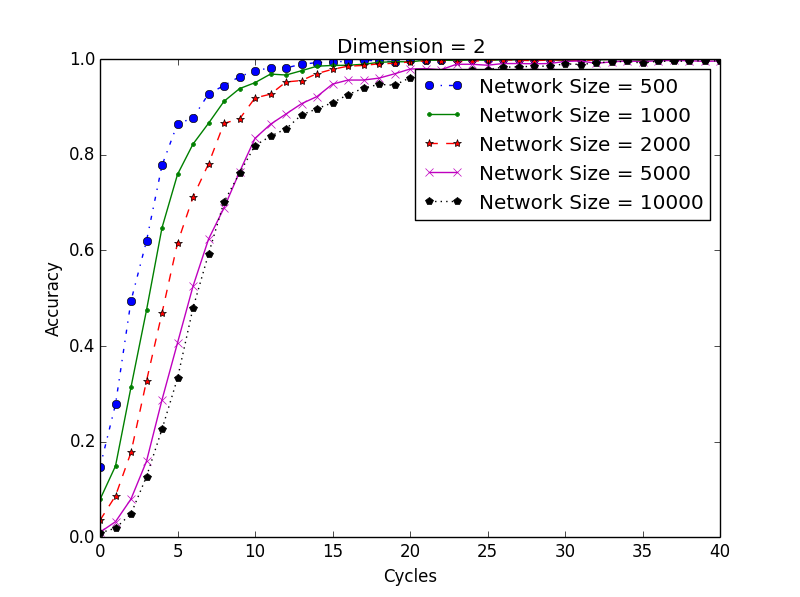
\includegraphics[width=\linewidth]{figs/conv_d2}
			\caption{This plot shows the accuracy rate of lookups on a 2-dimensional network as it self-organizes.}
			\label{fig:conv2}
		\end{subfigure} &

		\begin{subfigure}{0.5\columnwidth}
			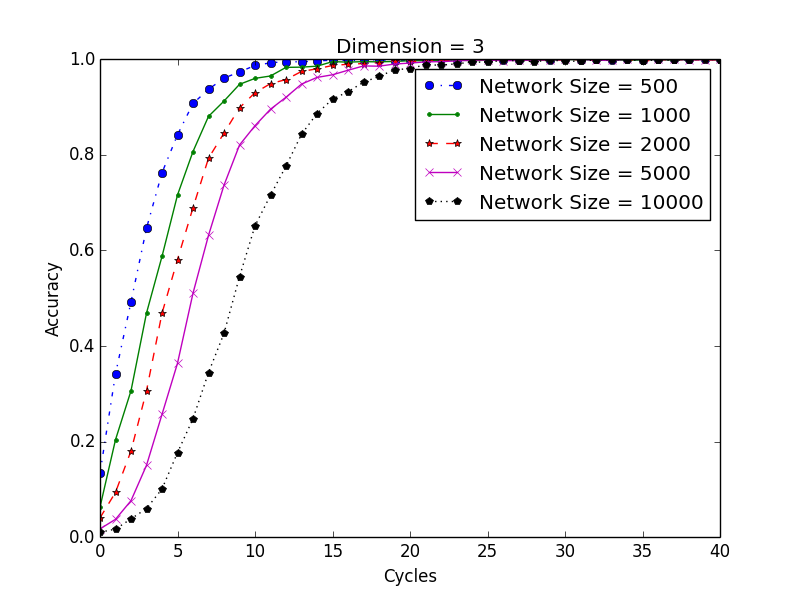
\includegraphics[width=\linewidth]{figs/conv_d3}
			\caption{This plot shows the accuracy rate of lookups on a 3-dimensional network as it self-organizes.}
			\label{fig:conv3}
		\end{subfigure} \\

		\begin{subfigure}{0.5\columnwidth}
			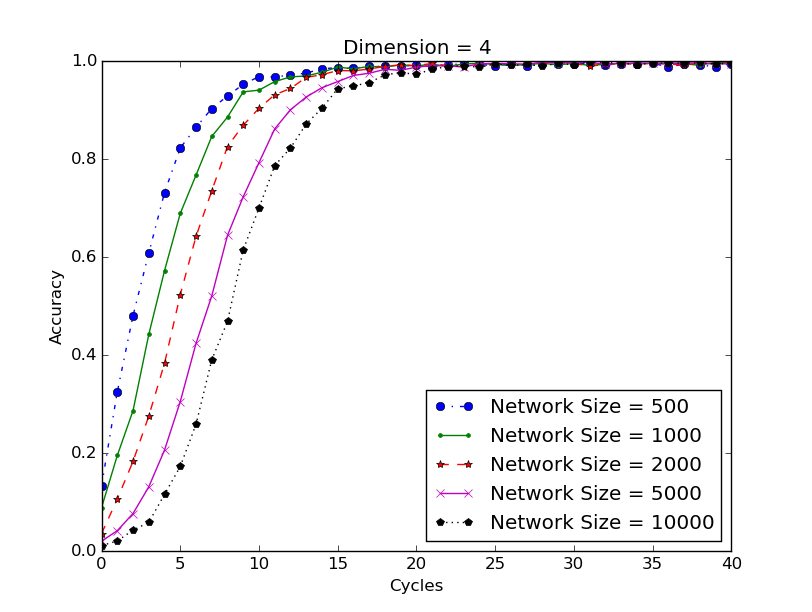
\includegraphics[width=\linewidth]{figs/conv_d4}
			\caption{This plot shows the accuracy rate of lookups on a 4-dimensional network as it self-organizes.}
			\label{fig:conv4}
		\end{subfigure} &


		\begin{subfigure}{0.5\columnwidth}
			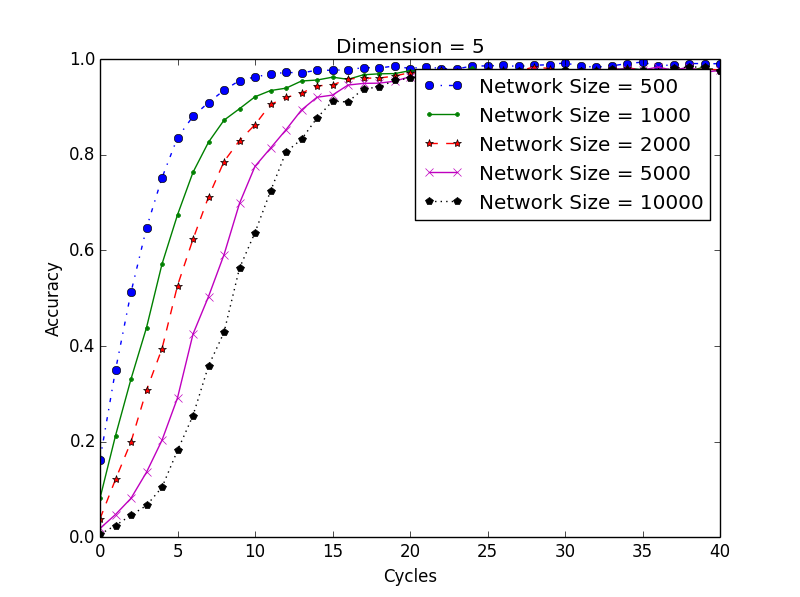
\includegraphics[width=\linewidth]{figs/conv_d5}
			\caption{This plot shows the accuracy rate of lookups on a 5-dimensional network as it self-organizes.}
			\label{fig:conv5}
		\end{subfigure}

	\end{tabular}
	\caption{These figures show that, starting from a randomized network, DGVH forms a stable and consistent network topology.
		The Y axis shows the success rate of lookups and the X axis show the number of gossips that have occurred.
		Each point shows the fraction of 2000 lookups that successfully found the correct destination.}
	
	\label{fig:conv}

\end{figure*}

\subsection{Latency Distribution Test}
The goal of our second set of experiments was to demonstrate VHash's ability to optimize a selected network metric: latency in this case.
In our simulation, we used the number of hops on the underlying network as an approximation of latency.
We compared VHash's performance to Chord \cite{chord}.
As we discussed in Chapter \ref{chapter:background} Chord is a well established DHT with an $O(\log(n))$ sized routing table and $O(\log(n))$ lookup time measured in overlay hops.

Instead of using the number of hops on the overlay network as our metric, we are concerned with the actual latency lookups experience traveling through the \emph{underlay} network, the network upon which the overlay is built.
Overlay hops are used in most DHT evaluations as the primary measure of latency.
It is the best approach available when there are no means of evaluating the characteristics of the underlying network.
VHash is designed with a capability to exploit the characteristics of the underlying network.
With most realistic network sizes and structures, there is substantial room for latency reduction in DHTs.

For this experiment, we constructed a scale free network with 10000 nodes placed at random (which has an approximate diameter of 3 hops) as an underlay network \cite{cohen2000resilience} \cite{pastor2001epidemic} \cite{hagberg2004}.
We chose to use a scale-free network as the underlay, since  scale free networks model the Internet's topology \cite{cohen2000resilience} \cite{pastor2001epidemic}.
We then chose a random subset of nodes to be members of the overlay network.
Our next step was to measure the distance in underlay hops between 10000 random source-destination pairs in the overlay.
VHash generated an embedding of the latency graph utilizing a distributed force directed model, with the latency function defined as the number of underlay hops between it and its peers.

Our simulation created 100, 500, and 1000 node overlays for both VHash and Chord.
We used 4 dimensions in VHash and a standard 160 bit identifier for Chord.




\begin{figure}

\begin{subfigure}{\columnwidth}
\centering
	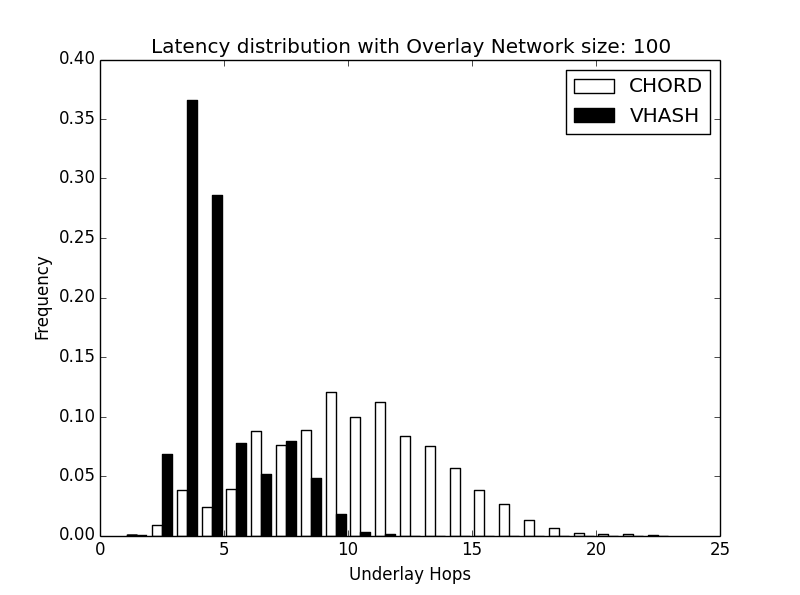
\includegraphics[width=0.5\linewidth]{figs/hist_100}
	\caption{Frequency of path lengths on Chord and VHash in a 100 node overlay.}
	\label{fig:hist100}
\end{subfigure}

\begin{subfigure}{\columnwidth}
	\centering
	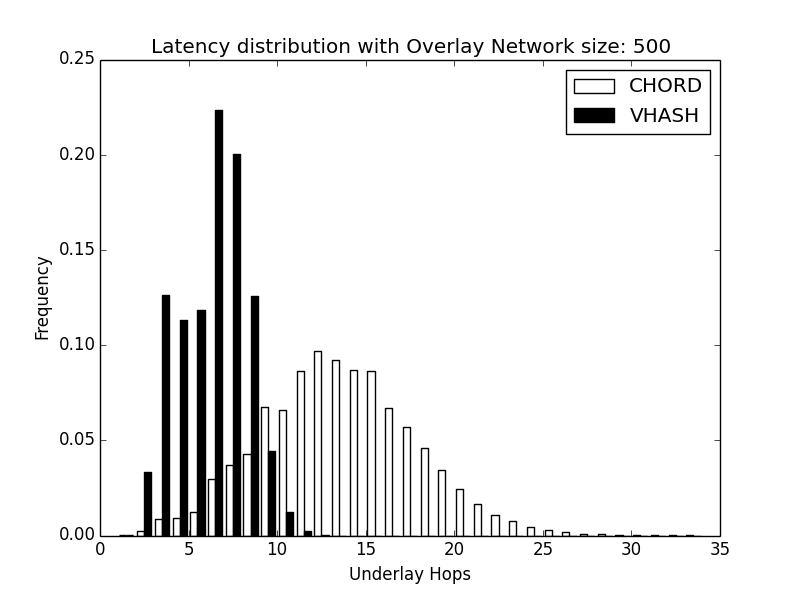
\includegraphics[width=0.5\linewidth]{figs/hist_500}
	\caption{Frequency of path lengths on Chord and VHash in a 500 node overlay.}
	\label{fig:hist500}
\end{subfigure}

\begin{subfigure}{\columnwidth}
	\centering
	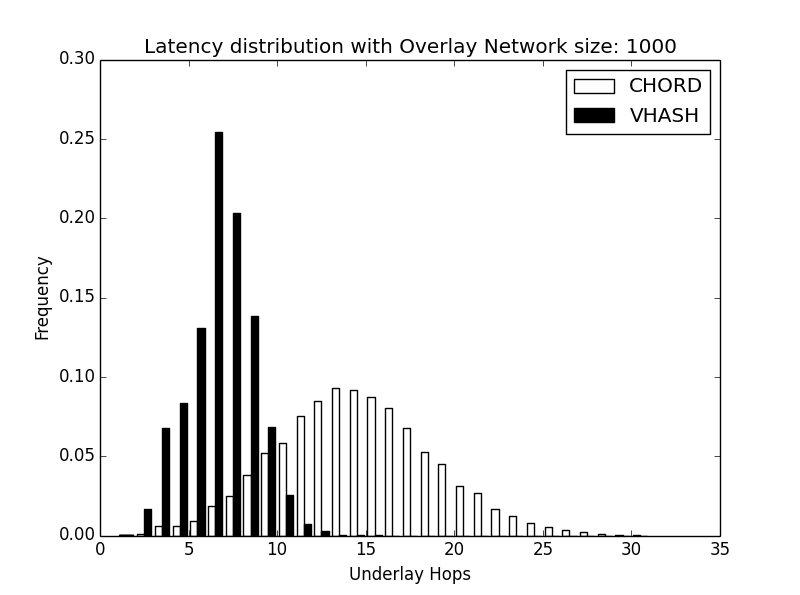
\includegraphics[width=0.5\linewidth]{figs/hist_1000}
	\caption{Frequency of path lengths on Chord and VHash in a 1000 node overlay.}
	\label{fig:hist1000}
\end{subfigure}

\caption{Figures \ref{fig:hist100}, \ref{fig:hist500}, and \ref{fig:hist1000} show the difference in the performance of Chord and VHash for 10,000 routing samples on a 10,000 node underlay network for differently sized overlays.
The Y axis shows the observed frequencies and the X axis shows the number of hops traversed on the underlay network.
VHash consistently requires fewer hops for routing than Chord.}
\label{fig:hist}

\end{figure}




Figure \ref{fig:hist} shows the distribution of path lengths measured in underlay hops in both Chord and VHash.
VHash significantly outperformed Chord and considerably reduced the underlay path lengths in three network sizes.

We also sampled the lookup length measured in overlay hops for a 1000 sized Chord and VHash network.
As seen in Figure \ref{fig:histover}, the paths measured in overlay for VHash were significantly shorter than those in Chord.
In comparing the overlay and underlay hops, we find that for each overlay hop in Chord, the lookup must travel 2.719 underlay hops on average; in VHash, lookups must travel 2.291 underlay hops on average for every overlay hop traversed.

Recall that this work is based on scale free networks, where latency improvements are difficult.
An improvement of 0.4 hops over a diameter of 3 hops is significant.
VHash has on average less overlay hops per lookup than Chord, and for each of these overlay hops we consistently traverse more efficiently across the underlay network.
\begin{figure}
	\centering
	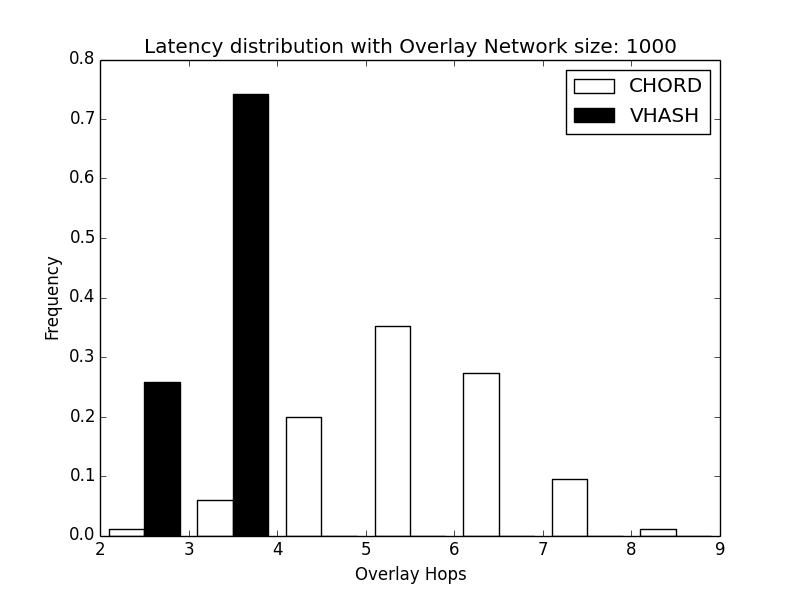
\includegraphics[width=0.5\linewidth]{figs/hist_overlay_4d}
	\caption{Comparison of Chord and VHash in terms of overlay hops.  Each overlay has 1000 nodes.  The Y axis denotes the observed frequencies of overlay hops and the X axis corresponds to the path lengths in overlay hops.}
	\label{fig:histover}
\end{figure}




\section{Remarks}

Voronoi tessellations have a wide potential for applications in ad-hoc networks, massively multiplayer games, P2P, and distributed networks.
However, centralized algorithms for Voronoi tessellation and Delaunay triangulation are not applicable to decentralized systems.
In addition, solving Voronoi tessellations in more than 2 dimensions is computationally expensive.

We created a distributed heuristic for Voronoi tessellations in an arbitrary number of dimensions.
Our heuristic is fast and scalable, with a expected memory cost of $(3d+1)^{2}+3d+1$ and expected maximum runtime of O$(\frac{\log^{2} N}{\log^{2} \log N} )$.

We ran two sets of experiments to demonstrate VHash's effectiveness.
Our first set of experiments demonstrated that our heuristic is reasonably accurate  and our second set demonstrates that reasonably accurate is sufficient to build a P2P network which can route accurately.
Our second experiment showed that VHash  could significantly reduced the latency in Distributed Hash Tables.

	\chapter{UrDHT}
\label{chapter:urdht}
%\begin{abstract}
As we have previously discussed, Distributed Hash Tables (DHTs) have an inherent set of qualities, such as greedy routing, maintaining lists of peers which define the topology, and forming an overlay network.
All DHTs use functionally similar protocols to perform lookup, storage, and retrieval operations.
Despite this, no one has created a cohesive formal DHT specification.

Our primary motivation for this project was to create an abstracted model for Distributed Hash Tables based on observations we made during previous research \cite{dgvh}.
We found that all DHTs can cleanly be mapped to the primal-dual problems of Voronoi Tessellation and Delaunay Triangulation.
Rather than having a developer be concerned with the details of a given DHT, we have constructed a new framework, UrDHT, that generalizes the functionality and implementation of various DHTs.

UrDHT is an abstract model of a Distributed Hash Table that implements a self-organizing web of computational units.
It maps the topologies of DHTs to the primal-dual problem of Voronoi Tessellation and Delaunay Triangulation.
By completing a few simple functions, a developer can implement the topology of any DHT in any arbitrary space using UrDHT.
For example, we implemented a DHT operating in a hyperbolic geometry, a previously unexplored nontrivial metric space with potential applications, such as latency embedding.

%Latency embedding will not be included in this paper
%One topology of particular interest we created is a DHT operating within a Poincar\'{e} disk model.
%This DHT could have latency embedded within the overlay and be capable of responding to changes in latency.
%The consequence of this is that, unlike other DHTs, the routing algorithm always uses the shortest latency path to a given destination.

	
%\end{abstract}

%\section{Introduction}
%%Distributed Hash Tables (DHT) have been extensively researched for the past decade.
%Many different DHT protocols have developed over the years.
%What is a DHT
% Mention the DHT API
%Despite this, no one has created a cohesive formal specification for building a DHT. % or something


%UrDHT is our specification and implementation of an abstract DHT.

%
%
%%We present UrDHT, an abstract model of a distributed hash table (DHT). %that solves a number of problems.
%%It is a unified and cohesive model for creating DHTs and P2P applications based on DHTs.
%%%UrDHT also provides a single network for bootstrapping distributed applications.
%%%Third, we show that using the abstraction features of UrDHT, we can embed latency into the DHT's overlay.
%%%
%%%\subsubsection{Abstraction}
%
%Distributed Hash Tables have been the catalyst for the creation of many P2P applications.
%Among these are Redis \cite{redis}, Freenet \cite{freenet}, and, most notably, BitTorrent \cite{bittorrent}. 
%
%
%%TODO Match vocabulary
%UrDHT builds its topology directly upon this insight.
%It uses a greedy distributed heuristic for approximating Delaunay Triangulations.
%We found that we could reproduce the topology of different DHTs by defining a selection heuristic and rejection algorithm for the geometry the DHT.
%For every DHT we implemented, our greedy approximation of Delaunay Triangulation produced a stable DHT, regardless of the geometry.  
%This works in non-Euclidean geometries such as XOR (Kademlia) or even a hyperbolic geometry represented by a Poincar\`{e} disc.
%
%The end result is not only do we have an abstract model of DHTs, we have a simple framework that developers can use to quickly create new distributed applications.
%This simple framework allows generation of internally consistent implementations of different DHTs that can have their performance rigorously compared.  %we can now test DHTs against each other fairly



%\subsubsection{Bootstrapping}
%Another poorly addressed issue within DHTs and DHT-based P2P applications we wish to tackle with UrDHT is the what we have termed the \textit{bootstrapping problem}.
%Simply put, a node can only join the network if it knows another node that is already a member of the network it is trying to join.
%%Current distributed systems suffer from fragmentation, high overhead, and an inability to scale due to difficulty of adoption.
%
%The way this generally works is by having a potential user manually look up at a centralized source, such as the project or application's website, the bootstrapping information for the network.
%It is a philosophical conflict requiring a distributed application to use a centralized source of information to build a distributed network.
%
%UrDHT has the potential to be a distributed source for bootstrapping information for other distributed networks.
%This would make new distributed applications easier to adopt by creating a network to bootstrap \textit{other networks}.
%UrDHT does this by making it easy to add other networks as a service.

%%\subsubsection*{Accomplishments}
%To summarize our contributions:
%\begin{itemize}
%	\item We give a formal specification for what needs to be defined in order to create a functioning DHT.
%	While there has long existed a well known protocol shared by distributed hash tables, this defines what a DHT does.
%	It does not describe what a DHT is.
%	
%	We show that DHTs cleanly map to the primal-dual problem of Delaunay Triangulation and Voronoi Tessellation.
%	We list a set of simple functions that, once defined, allow our Distributed Greedy Voronoi Heuristic (DGVH) to be run in any space, creating a DHT overlay for that space (Section \ref{sec:define}).
%	
%	\item We present UrDHT as an abstract DHT and show how a developer would modify the functions we defined to create an arbitrary new DHT topology (Section \ref{sec:urdht}).
%	
%	\item We show how to reproduce the topology of Chord and Kademlia using UrDHT.
%	We also implement a DHT in a Euclidean geometry and a hyperbolic geometry represented by a Poincar\`{e} disc (Section \ref{sec:implement}).
%%	We also discuss how we can use UrDHT to run subnetworks as a service.
%	\item We conduct experiments that show building DHTs using UrDHT produced efficiently routable networks, regardless of the underlying geometry(Section \ref{sec:experiments}). 
%	\item We present some efforts and projects that are similar to our own (Section \ref{sec:related}).
%	\item We discuss the ramifications of our work and what future work is available (Section \ref{sec:future}).
%\end{itemize}


\section{What Defines a DHT}
\label{sec:define}

A distributed hash table is usually defined by its protocol; in other words, what it can do.
Nodes and data in a DHT are assigned unique\footnote{Unique with astronomically high probability, given a large enough consistent hashing algorithm.} keys via a consistent hashing algorithm.
To make it easier to intuitively understand the context, we will call the key associated with a node its ID and refer to nodes and their IDs interchangeably.

A DHT can perform the \texttt{lookup(key)}, \texttt{get(key)}, and \texttt{store(key, value)} operations.\footnote{There is typically a \textit{delete(key)} operation too, but it is not strictly necessary.}
The \texttt{lookup} operation returns the node responsible for a queried key.
The \texttt{store} function stores that key/value pair in the DHT, while \texttt{get} returns the value associated with that key.

However, these operations define the functionality of a DHT, but do not define the requirements for implementation.
We define the necessary components that comprise DHTs.
We show that these components are essentially Voronoi Tessellation and Delaunay Triangulation.

\subsection{DHTs, Delaunay Triangulation, and Voronoi Tessellation}

Nodes in different DHTs have, what appears at the first glance, wildly disparate ways of keeping track of peers - the other nodes in the network.
However, peers can be split into two groups.

The first group is the \textit{short peers}.
These are the closest peers to the node and define the range of keys the node is responsible for. 
A node is responsible for a key if and only if its ID is closest to the given key in the geometry of the DHT.
Short peers define the DHTs topology and guarantee that the greedy routing algorithm shared by all DHTs works.


%All other peers comprise the \textit{long peers}.
Long peers are the nodes that allow a DHT to achieve faster routing speeds than the topology would allow using only short peers.
This is typically $ O(\log(n)) $ hops, although polylogarithmic time is acceptable \cite{kleinberg2000small}.
A DHT can still function without long peers.

Interestingly, despite the diversity of DHT topologies and how each DHT organizes short and long peers,  all DHTs use functionally identical greedy routing algorithms (Algorithm \ref{alg:routing}):

\begin{algorithm}
	\caption{The DHT Generic Routing algorithm}
	\label{alg:routing}
	%\algsetup{linenosize=\tiny}
	\small
	\begin{algorithmic}[1]
%		\State Given node $n$ and a message being sent to $key$
		\Function{ $n.$lookup}{$(key)$}
			\If{$key \in n$'s range of responsibility}
				\State \Return $ n $
			\EndIf
			\If{ One of $n$'s short peers is responsible for $key$}
				\State \Return the responsible node
			\EndIf
			\State $ candidates $ = $ short\_peers $ + $ long\_peers $
			\State $ next  \leftarrow $  $\min (n$.distance($candidates$, $ key ))$
			\State \Return $next.$lookup($key$)
		\EndFunction
	\end{algorithmic}
	
	\scriptsize
\end{algorithm}
The algorithm is as follows:
If I, the node, am responsible for the key, I return myself.
Otherwise, if I know who is responsible for this key, I return that node.
Finally, if that is not the case, I forward this query to the node I know with shortest distance from the node to the desired key.\footnote{This order matters, as some DHTs such as Chord are unidirectional.} 

Depending of the specific DHT, this algorithm might be implemented either recursively or iteratively.
It will certainly have differences in how a node handles errors, such as how to handle connecting to a node that no longer exists.
This algorithm may possibly be run in parallel, such as in Kademlia \cite{kademlia}.
The base greedy algorithm is always the same regardless of the implementation.


\begin{figure}
	\centering
	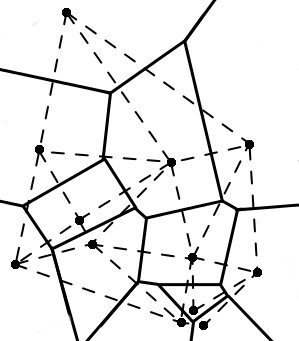
\includegraphics[width=0.75\linewidth]{figs/voronoi}
	\caption{An example Voronoi diagram for objects on a 2-dimensional space.  The black lines correspond to the borders of the Voronoi region, while the dashed lines correspond to the edges of the Delaunay Triangulation.}
	\label{fig:voro-ex}
\end{figure}


With the components of a DHT defined above, we can now show the relationship between DHTs and the primal-dual problems of Delaunay Triangulation and Voronoi Tessellation.
An example Delaunay Triangulation and Voronoi Tessellation is show in Figure \ref{fig:voro-ex}.

%TODO A one-dimensional voronoi fig as example
We can map a given node's ID to a point in a space and the set of short peers to the Delaunay Triangulation.
This would make the range of keys a node is responsible correspond to the node's Voronoi region.
Long peers serve as shortcuts across the mesh formed by Delaunay Triangulation.


Thus, if we can calculate the Delaunay Triangulation between nodes in a DHT, we have a generalized means of creating the overlay network.
This can be done with any algorithm that calculates the Delaunay Triangulation.

Computing the Delaunay Triangulation and/or the Voronoi Tessellation of a set of points is a well analyzed problem.
Many algorithms exist which efficiently compute a Voronoi Tessellation for a given set of points on a plane, such as Fortune's sweep line algorithm \cite{fortune1987sweepline}.

However, DHTs are completed decentralized, with no single node having global knowledge of the topology.
Many of the algorithms to compute Delaunay Triangulation and/or Voronoi Tessellation are unsuited to a distributed environment.
In addition, the computational cost increases when we move into spaces with greater than two dimensions.
In general, finding the Delaunay Triangulation of $n$ points in a space with $d$ dimensions takes $O(n^{\frac{2d-1}{d}})$ time \cite{watson1981computing}.


Is there an algorithm we can use to efficiently calculate Delaunay Triangulation for a distributed system in an arbitrary space?
We created an algorithm called the Distributed Greedy Voronoi Heuristic (DGVH), explained below \cite{dgvh}.


\subsection{Distributed Greedy Voronoi Heuristic}
\label{sec:dgvh}


The Distributed Greedy Voronoi Heuristic (DGVH) is an efficient method for nodes to approximate their individual Voronoi region (Algorithm \ref{alg:dgvh}). 
DGVH selects nearby nodes that would correspond to points connected to it within a Delaunay Triangulation.
Our previous implementation relied on a midpoint function \cite{dgvh}.
We have refined our heuristic to render a midpoint function unnecessary.

The heuristic is described in Algorithm \ref{alg:dgvh}.
Every maintenance cycle, nodes exchange their peer lists with their short peers.
A node creates a list of candidates by combining their peer lists with their neighbor's peer lists.\footnote{In our previous paper, nodes exchange short peer lists with a single peer. Calls to DGVH in this paper use both short and long peer information from all of their short peers.}
Sort the list of peers from closest to furthest distance.
The node then initializes a new peer list, initially containing the closest candidate.
For each of the remaining candidates, the node compares the distance between the current short peers and the candidate.
If the new peer list does not contain any short  peers closer to the candidate than the node, the candidate is added to the new peer list.
Otherwise, the candidate is set aside.

The resulting short peers are a subset of the node's actual Delaunay neighbors.
A crucial feature is that this subset guarantees that DGVH will form a routable mesh.


\begin{algorithm} % make smaller
	\caption{Distributed Greedy Voronoi Heuristic}
	\label{alg:dgvh}
%	\algsetup{linenosize=\tiny}
	\small
	\begin{algorithmic}[1]  % the numberis how many lines
		\State Given node $n$ and its list of $candidates$.
		\State Given the minimum $table\_size$
		\State $short\_peers \leftarrow$ empty set% that will contain $n$'s one-hop peers
		\State $long\_peers \leftarrow$ empty set %that will contain $n$'s peers further than one hop.
		\State Sort $candidates$ in ascending order by each node's \texttt{distance} to $n$
		\State Remove the first member of $candidates$ and add it to $short\_peers$
		\ForAll {$c$ in $candidates$}
			\If{any node in $short\_peers$ is closer to $c$ than $n$}
				\State Reject $c$ as a peer
			\Else
				\State Remove $c$ from $candidates$
				\State Add $c$ to $short\_peers$
			\EndIf
		\EndFor
		\While{$|short\_peers| < table\_size $ and $ |candidates| >0$}
			\State Remove the first entry $c$ from $candidates$
			\State Add $c$ to $short\_peers$
		\EndWhile
		\State Add $candidates$ to the set of $long\_peers$	
		\State \texttt{handleLongPeers}($long\_peers$)
		%\IF{$|long\_peers| > table\_size^2$}
		%	\State $long\_peers \leftarrow$ random subset of $long\_peers$ of size $table\_size^2$
		%\ENDIF
	\end{algorithmic}
\end{algorithm} 


Candidates are gathered via a gossip protocol as well as notifications from other peers.
How long peers are handled depends on the particular DHT implementation.
This process is described more in Section \ref{sec:protocol}.

The expected maximum size of $ candidates $ corresponds to the expected maximum degree of a vertex in a Delaunay Triangulation.
This is  $\Theta(\frac{\log n}{\log \log n} )$, regardless of the number of the dimensions \cite{bern1991expected}. 
We can therefore expect \textit{short peers} to be bounded by $\Theta(\frac{\log n}{\log \log n})$.

The expected worst case cost of DGVH is \(O(\frac{\log^{4} n}{\log^{4} \log n} )\) \cite{dgvh}, regardless of the dimension \cite{dgvh}.\footnote{As mentioned in the previous footnote, if we are exchanging only short peers with a single neighbor rather than all our neighbors, the cost lowers to \(O(\frac{\log^{2} n}{\log^{2} \log n} )\).}
In most cases, this cost is much lower.
Additional details can be found in our previous work \cite{dgvh}.




We have tested DGVH on Chord (a ring-based topology), Kademlia (an XOR-based tree topology), general Euclidean spaces, and even in a hyperbolic geometry.
This is interesting because not only can we implement the contrived topologies of existing DHTs, but more generalizable topologies like Euclidean or hyperbolic geometries.
We show in Section \ref{sec:experiments} that DGVH works in all of these spaces.
DGVH only needs the distance function to be defined in order for nodes to perform lookup operations and determine responsibility.
%TODO This is where we need to match vocab
%\begin{itemize}
%	\item \textbf{A \texttt{distance} function } - This measures distance in the overlay formed by the Distributed Hash Table.
%	In most DHTs, the distance in the overlay has no correlation with real-world attributes.
%	
%	\item \textbf{A \texttt{responsibility} definition}  This defines the range of keys a node is responsible for. 
%	Not every DHT defines which node is responsible for particular keys in the same way. 
%	For example, nodes in Kademlia are responsible for the keys closest to themselves, while in Chord, nodes are responsible for the keys falling between themselves and the preceding node.
%\end{itemize}
We will now show how we used this information and heuristic to create UrDHT, our abstract model for distributed hash tables.





\section{UrDHT}
\label{sec:urdht}


The name UrDHT comes from the German prefix \textit{ur}, which means ``original.'' 
The name is inspired by UrDHT's ability to reproduce the topology of other distributed hash tables.

UrDHT is divided into 3 broad components: Storage, Networking, and Logic.
Storage handles file storage and Networking dictates the protocol for how nodes communicate.
These components oversee the lower level mechanics of how files are stored on the network and how bits are transmitted through the network.
The specifics are outside the scope of the paper, but can be found on the UrDHT Project site \cite{urdht}.

Most of our discussion will focus on the Logic component.
The Logic component is what dictates the behavior of nodes within the DHT and the construction of the overlay network.
It is composed of two parts: the DHT Protocol and the Space Math.

The DHT Protocol contains the canonical operations that a DHT performs, while the Space Math is what effectively distinguishes one DHT from another.
A developer only needs to change the details of the \texttt{space math} package in UrDHT to create a new type of DHT.
We discuss each in further detail below.

\subsection{The DHT Protocol }
\label{sec:protocol}

The DHT Protocol (\texttt{LogicClass.py}) \cite{urdht} is the shared functionality between every single DHT.
It consists of the node's information, the short peer list that defines the minimal overlay, the long peers that make efficient routing possible, and all the functions that use them.
There is no need for a developer to change anything in the DHT Protocol, but it can be modified if so desired.
The DHT Protocol depends on functions from Space Math in order to perform operations within the specified space.

Many of the function calls should be familiar to anyone who has study DHTs.
We will discuss a few new functions we added and the ones that contribute to node maintenance.



The first thing we note is the absence of \texttt{lookup}.
In our efforts to further abstract DHTs, we have replaced \texttt{lookup} using the function \texttt{seek}.
The \texttt{seek} function acts a single step of \texttt{lookup}.
It returns the closest node to $ key $ that the node knows about.

Nodes can perform \texttt{lookup} by iteratively calling \texttt{seek} until it receives the same answer twice.
We do this because we make no assumptions as to how a client using a DHT would want to perform lookups and handle errors that can occur.
It also means that a single client implementing \texttt{lookup} using iterative \texttt{seek} operations could traverse any DHT topology implemented with UrDHT.

%We also slightly modified the assumptions of how \texttt{join} works.
%The \texttt{join} operation takes in a set of bootstrap nodes, called $ candidates$, rather than a single node.
%%This is part of our plans about how UrDHT can be used as a bootstrap network by providing bootstrapping information for a particular network.
%%We expect nodes that want to join a particular network to be able to query UrDHT and receive a list of nodes that they can use to bootstrap the joining.
%
%The joining node randomly selects one of these $ candidates $ and finds the ``parent'' node currently responsible for the space.
%The joining node then populates its short peers using the ``parent'' node's short peers.
%The node  uses the parent to populate its short peer list and then makes it aware of its existence using \texttt{notify}.
%Once that has been finished, the joining node starts its maintenance thread.
%
%


Maintenance is done via gossip.
Each maintenance cycle, the node recalculates its Delaunay (short) peers using its neighbors' peer lists and any nodes that have notified it since the last maintenance cycle.
Short peer selection are done using DGVH by default.
While DGVH has worked in every single space we have tested, this is not proof it will work in every single case.
It is reasonable and expected that some spaces may require a different Delaunay Triangulation calculation or approximation method.

Once the short peers are calculated, the node handles modifying its long peers.
This is done using the \texttt{handleLongPeers} function described in Section \ref{sec:space}.

\subsection{The Space Math}
\label{sec:space}
The Space Math consists of the functions that define the DHT's topology.
It requires a way to generate short peers to form a routable overlay and a way to choose long peers.
%We use DGVH for generating short peers, which works in every space tested.
Space Math requires the following functions when using DGVH:

\begin{itemize}

%\subsubsection{IDToPoint}
\item The \texttt{idToPoint} function takes in a node's ID and any other attributes needed to map an ID onto a point in the space.
The ID is generally a large integer generated by a cryptographic hash function.
%In the vast majority of DHTs, this \texttt{idToPoint} function needs nothing more than the ID as input.
%The ID is directly translated into a large integer and used as a coordinate in a one dimensional space.


%\subsubsection{Distance}
\item The \texttt{distance} function takes in two points, $a$ and $b$, and outputs the shortest distance from $a$ to $b$.
This distinction matters, since distance is not symmetric in every space.
The prime example of this is Chord, which operates in a unidirectional toroidal ring.



%\subsubsection{Get Closest}
%Depending on what you want to measure, \texttt{getClosest} might measure the distance from $ center$ to each of the candidates or from each of the candidates to the $ center$.

%\subsubsection{Get Delaunay (short) Peers}
\item We use the above functions to implement \texttt{getDelaunayPeers}.
Given a set of points, the $ candidates$, and a center point $ centers$, \texttt{getDelaunayPeers} calculates a mesh that approximates the Delaunay peers of $ center$.
We assume that this is done using DGVH (Algorithm \ref{alg:dgvh}).



\item The function \texttt{getClosest} returns the point closest to $ center$ from a list of $ candidates$, measured by the distance function.
The \texttt{seek} operation depends on the \texttt{getClosest} function.


%\subsubsection{Handle Long Peers}



\item The final function is \texttt{handleLongPeers}.
\texttt{handleLongPeers} takes in a list of $ candidates $ and a $ center$, much like \texttt{getDelaunayPeers}, and returns a set of peers to act as the routing shortcuts.

The implementation of this function should vary greatly from one DHT to another.
For example, Symphony \cite{symphony} and other small-world networks \cite{kleinberg2000navigation} choose long peers using a probability distribution.
Chord has a much more structured distribution, with each long peer being increasing powers of 2 distance away from the node \cite{chord}.
The default behavior is to use all candidates not chosen as short peers as long peers, up to a set maximum.
If the size of long peers would exceed this maximum, we instead choose a random subset of the maximum size, creating a naive approximation of the long links in the Kleinberg small-world model \cite{kleinberg2000navigation}.
Long peers do not greatly contribute to maintenance overhead, so we chose 200 long peers as a default maximum.

%In some case it may more convenient implement \texttt{handleLongPeers} as part of \texttt{getDelaunayPeers}.

\end{itemize}


%\subsubsection*{Put and Poll}
%The functions of \texttt{store} and \texttt{get} can be further abstracted otu to \texttt{put} and \texttt{poll}


%This does X


\section{Implementing other DHTs}
\label{sec:implement}
\subsection{Implementing Chord}

Ring topologies are fairly straightforward since they are one dimensional Voronoi Tessellations, splitting up what is effectively a modular number line among multiple nodes.

Chord uses a unidirectional distance function.
Given two integer keys $ a $ and $ b $ and a maximum value $ 2^{m}$, the \texttt{distance} from $ a $ to $ b $ in Chord is: 
\[ distance(a,b) =
\begin{cases}
	2^m + b - a, & \text{if } b - a < 0 \\
	b-a, & \text{otherwise}
\end{cases}
  \]


Short peer selection is trivial in Chord, so rather than using DGVH for \texttt{getDelaunayPeers}, each node chooses from the list of candidates the candidate closest to it (predecessor) and the candidate to which it is closest (successor).

Chord's finger (long peer) selection strategy is emulated by \texttt{handleLongPeers}.
For each of the $i$th bits in the hash function, we choose a long peer $ p_i $ from the candidates such that 


\[ p_i =   getClosest\left(candidates, t_{i}\right)  \]
where
\[t_{i} =  (n + 2^{i}) \mod 2^m \]
for the current node $n$.
The \texttt{getClosest} function in Chord should return the candidate with the shortest distance from the candidate to the point.

This differs slightly from how selects its long peers.
In Chord, nodes actively seek out the appropriate long peer for each  corresponding bit.
In our emulation, this information is propagated along the ring using short peer gossip.


%for i in range(0, HASHBASE):
%target = tuple([(center[0] + 2**i) % HASHMAX])
%subject = min(others, key=lambda x: chordDist(x.loc, target))
%We know Chord's invariants are not (citation), but our protocol isn't affected by these constraints


\subsection{Implementing Kademlia}
Kademlia uses the exclusive or, or XOR, metric for distance.
This metric, while non-euclidean, is perfectly acceptable for calculating distance.
For two given keys $ a $ and $ b $

\[ distance(a, b) = a  \oplus b\]

The \texttt{getDelaunayPeers} function uses DGVH as normal to choose the short peers for node $n$.
We then used Kademlia's $k$-bucket strategy \cite{kademlia} for \texttt{handleLongPeers}.
The remaining candidates are placed into buckets, each capable holding a maximum of $k$ long peers.

To summarize briefly, node $n$ starts with a single bucket containing itself, covering long peers for the entire range.
When attempting to add a candidate to a bucket already containing $k$ long peers, if the bucket contains node $n$, the bucket is split into two buckets, each covering half of that bucket's range.
Further details of how Kademlia $k$-buckets work can be found in the Kademlia protocol paper \cite{kademlia}.


\subsection{ZHT}
ZHT \cite{li2013zht} leads to an extremely trivial implementation in UrDHT.
Unlike other DHTs, ZHT assumes an extremely low rate of churn.
It bases this rationale on the fact that tracking $ O(n) $ peers in memory is trivial.
This indicates the $ O( \log n)  $  memory  requirement for other DHTs is overzealous and not based on a memory limitation.
Rather, the primary motivation for keeping a number of peers in memory is more due to the cost of maintenance overhead.
ZHT shows, that by assuming low rates of churn (and infrequent maintenance messages as a result), having $O(n)$ peers is a viable tactic for faster lookups.

As a result, the topology of ZHT is a clique, with each node having an edge to all other nodes.
This yields $ O(1) $ lookup times with an $ O(n) $ memory cost.
The only change that needs to be made to UrDHT is to accept all peer candidates as short peers.

\subsection{Implementing a DHT in a non-contrived Metric Space}

We used a Euclidean geometry as the default space when building UrDHT and DGVH \cite{dgvh}.
For two vectors $\vec{a}$ and $\vec{b}$ in $d$ dimensions: 

\[distance\left(\vec{a}, \vec{b}\right) = \sqrt{\sum\limits_{i\in d} \left(a_i-b_i\right)^2}\]


We implement \texttt{getDelaunayPeers} using DGHV and set the minimum number of short peers to $3d+1$, a value we found through experimentation \cite{dgvh}.

Long peers are randomly selected from the left-over candidates after DGVH is performed \cite{dgvh}.
The maximum size of long peers is set to $(3d+1)^2$, but it can be lowered or eliminated if desired and maintain $ O(\sqrt[d]{n}) $ routing time.


Generalized spaces such as Euclidean space allow the assignment of meaning to arbitrary dimension and allow for the potential for efficient querying of a database stored in a DHT.

%\subsection{Implementing a DHT in a Hyperbolic Geometry}
	
\label{sec:hyper}

We have already shown with Kademlia that UrDHT can operate in a non-Euclidean geometry.
Another non-euclidean geometry UrDHT can work in is a hyperbolic geometry.

We implemented a DHT within a hyperbolic geometry using a Poincar\`{e} disc model.
To do this, we implemented \texttt{idToPoint} to create a random point in Euclidean space from a uniform distribution.
This point is then mapped to a Poincar\`{e} disc model to determine the appropriate Delaunay peers.
For any two given points $a$ and $b$ in a Euclidean vector space, the \texttt{distance} in the  Poincar\`{e} disc is:


\[ distance(a, b) = \operatorname{arcosh} \left(  1+ 2 \frac{ \left\| a - b \right\| ^{2} }{ ( 1 - \left\| a \right\| ^{2} ) ( 1 - \left\| b \right\| ^{2} ) }\right) \]


Now that we have a \texttt{distance} function, DGVH can be used in \texttt{getDelaunayPeers} to generate an approximate Delaunay Triangulation for the space.
The \texttt{getDelaunayPeers} and \texttt{handleLongPeers} functions are otherwise implemented exactly as they were for Euclidean spaces. 




Implementing a DHT in hyperbolic geometry has many interesting implications.
Of particular note, embedding into hyperbolic spaces allows us to explore accurate embeddings of internode latency into the metric space \cite{kleinberg2007geographic} \cite{cvetkovski2009hyperbolic}.
This has the potential to allow for minimal latency DHTs.


%\subsection{Services}
%
%There needs to be an easy way to append data to the bootstrapping list.
%
%To do this, we introduce the \texttt{put} and  \texttt{poll} primitives.
%These functions can considered abstracted versions.
%	
\section{Experiments}
\label{sec:experiments}

We use simulations to test our implementations of DHTs using UrDHT.
Using simulations to test the correctness and relative performance of DHTs is standard practice for testing and analyzing DHTs \cite{kademlia} \cite{symphony} \cite{chord}  \cite{tapestry}  \cite{raynet} \cite{li2005comparing}.

%Tests
%k connected randomly populated network
%vars:
%k for your k connected network 10, 20
%duration what we have works
%size 100, 500, 1000, 5000 if possible,
%
%Iterative joins, start with one node
%vars:  join rate (ticks per join) ,1 3 
%final size  100, 500, 1000, 5000 if possible,
%join method (bootstrapping size)  all,
%
%outputs
%Network diameter at tick
%avg greedy routing distance
%greedy routing success rate at tick
%maximum degree
%mean degree
%std deviatation degree
%Anything we want for degree
%
%
%Graph max degree vs expected  maximimum degree  (this is short peers)

%\subsection{Experimental Setup}
We tested four different topologies: Chord, Kademlia, a Euclidean geometry, and a Hyperbolic geometry.
For Kademlia, the size of the $k$-buckets was 3.
In the Euclidean and Hyperbolic geometries, we set a minimum of 7 short peers and a maximum of 49 long peers.

We created 500 node networks, starting with a single node and adding a node each maintenance cycle.\footnote{We varied the amount of maintenance cycles between joins in our experiments, but found it had no effect upon our results.}

For each topology, at each step, we measured:
\begin{itemize}
	\item The average degree of the network.  This is the  number of outgoing links and includes both short and long peers.
	\item The worst case degree of the network.
	\item The average number of hops between nodes using greedy routing.
	\item The diameter of the network.  
	This is the worst case distance between two nodes using greedy routing.
\end{itemize}

We also tested the reachability of nodes in the network.
At every step, the network is fully reachable.

Results generated by the Chord and Kademlia simulations were in line with those from previous work  \cite{kademlia} \cite{chord}.
This demonstrates that UrDHT is capable of accurately emulating these topologies.
We show these results in Figures \ref{fig:ChordDegree} - \ref{fig:KademliaDistance}.



\begin{figure}
	\centering
	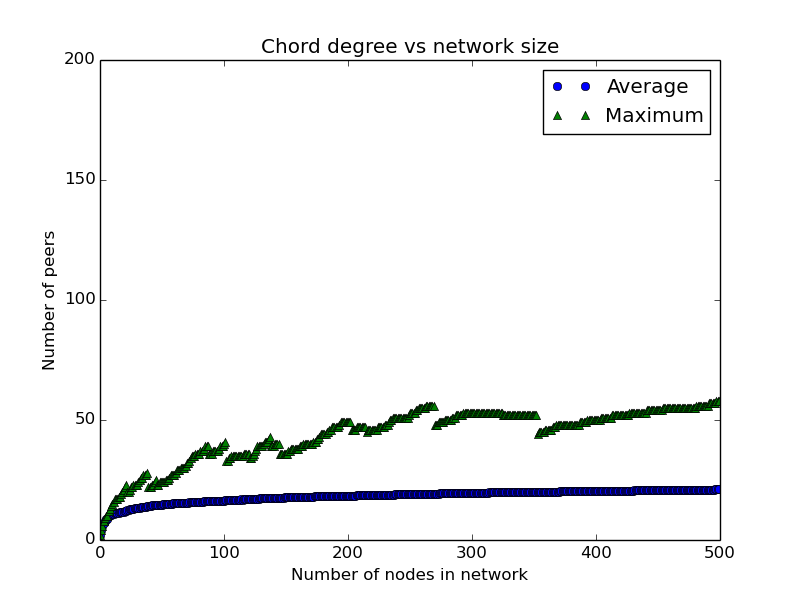
\includegraphics[width=\linewidth]{figs/ChordDegree}
	\caption{This is the average and maximum degree of nodes in the Chord network. This Chord network utilized a 120 bit hash and thus degree is bound at 122 (full fingers, predecessor and successor) when the network reaches $2^{120}$ nodes.}
	\label{fig:ChordDegree}
\end{figure}

\begin{figure}
	\centering
	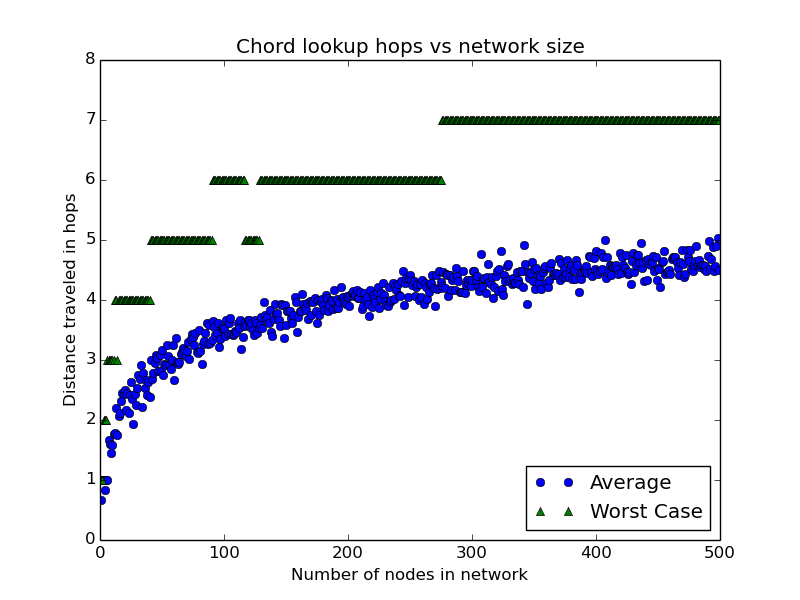
\includegraphics[width=\linewidth]{figs/ChordDistance}
	\caption{This is the number hops required for a greedy routed lookup in Chord. The average lookup between two nodes follows the expected logarithmic curve.}
	\label{fig:ChordDistance}
\end{figure}

\begin{figure}
	\centering
	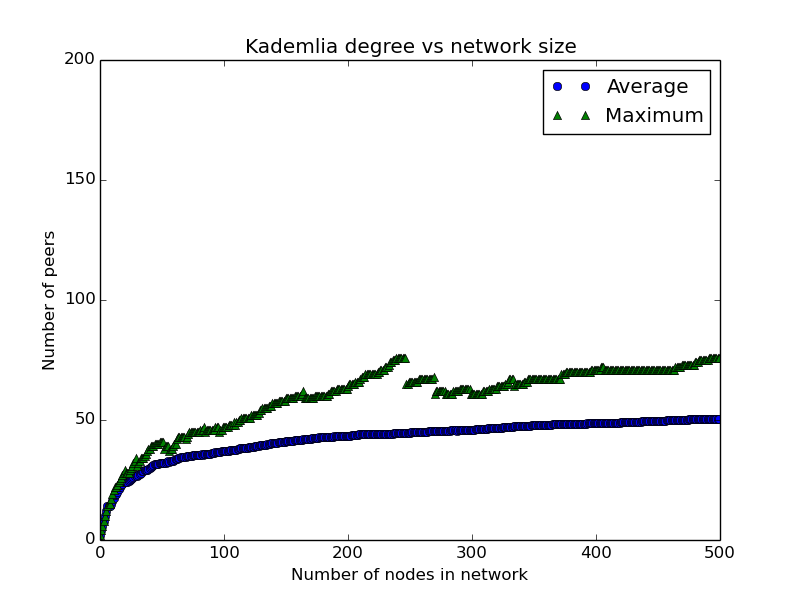
\includegraphics[width=\linewidth]{figs/KademliaDegree}
	\caption{This is the average and maximum degree of nodes in the Kademlia network as new nodes are added.  Both the maximum degree and average degree are $O(\log n)$.}
	\label{fig:KademliaDegree}
\end{figure}
\begin{figure}
	\centering
	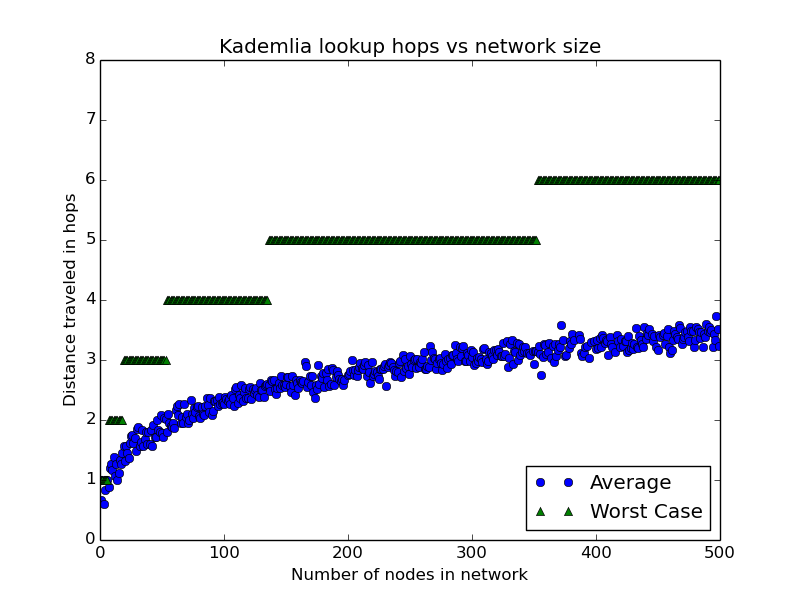
\includegraphics[width=\linewidth]{figs/KademliaDistance}
	\caption{Much like Chord, the average degree follows a distinct logarithmic curve, reaching an average distance of approximately three hops when there are 500 nodes in the network.}
	\label{fig:KademliaDistance}
\end{figure}



The results of our Euclidean and Hyperbolic geometries indicate similar asymptotic behavior: a higher degree produces a lower diameter and average routing. 
However, the ability to leverage this trade-off is limited by the necessity of maintaining an $ O(\log n $) degree.
These results are shown in Figures \ref{fig:EucldianDegree} - \ref{fig:HyperbolicDistance}.

While we maintain the number of links must be $ O(\log n)$, all DHTs practically bound this number by a constant.  
For example, in Chord, this is the number of bits in the hash function plus the number of predecessors/successors.
Chord and Kademlia fill this bound asymptotically. 
The long peer strategy used by the Euclidean and Hyperbolic metrics aggressively filled to this capacity, relying on the distribution of long peers to change as the network increased in size rather than increasing the number of utilized long peers.
This explains why the Euclidean and Hyperbolic spaces have more peers (and thus lower diameter) for a given network size.
This presents a strategy for trade-off of the network diameter vs. the overhead maintenance cost.


%\subsection{Chord}
%Our model of Chord
%\cite{chord}.


\begin{figure}
\centering
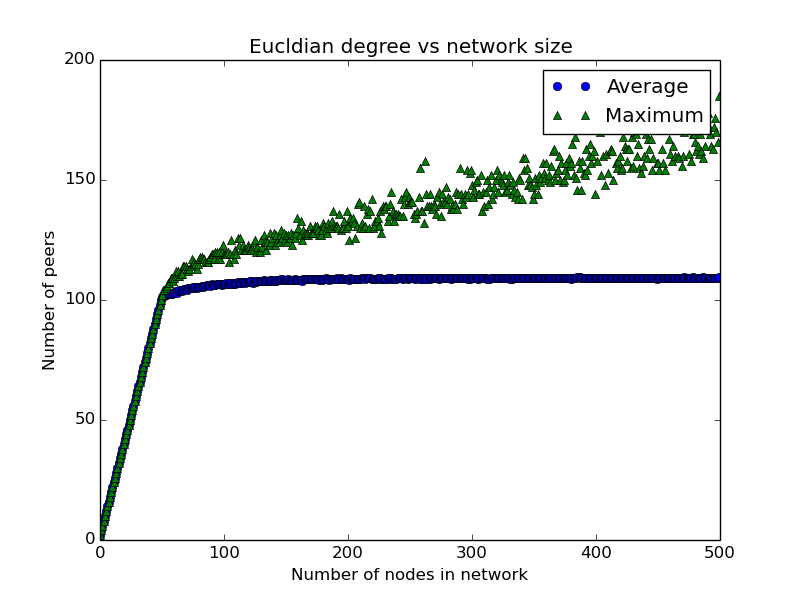
\includegraphics[width=\linewidth]{figs/EucldianDegree}
\caption{Because the long peers increase linearly to the maximum value (49), degree initially rises quickly and then grows  more slowly as the number of long peers ceases to grow and the size short peers increases with network size. }
\label{fig:EucldianDegree}
\end{figure}

\begin{figure}
\centering
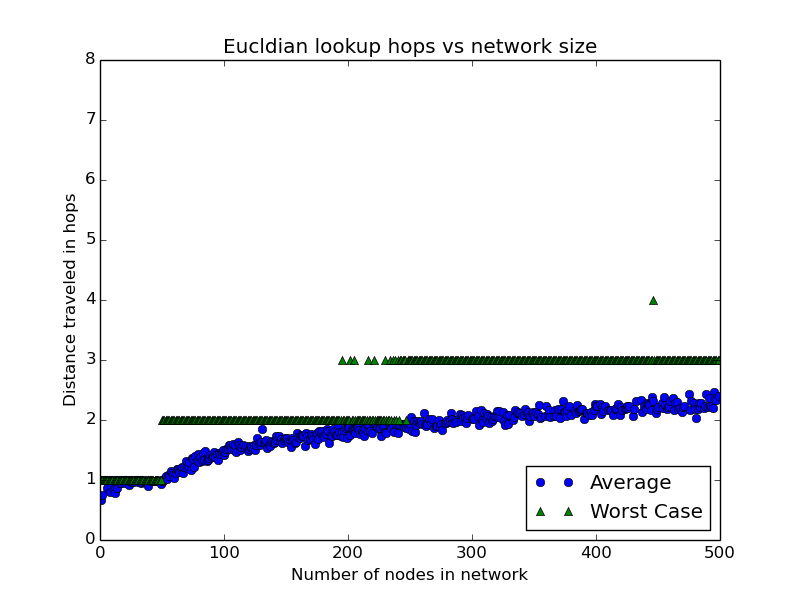
\includegraphics[width=\linewidth]{figs/EucldianDistance}
\caption{The inter-node distance stays constant at 1 until long peers are filled, then rises at the rate of a randomly connected network due to the distribution of long peers selected}
\label{fig:EucldianDistance}
\end{figure}

\begin{figure}
\centering
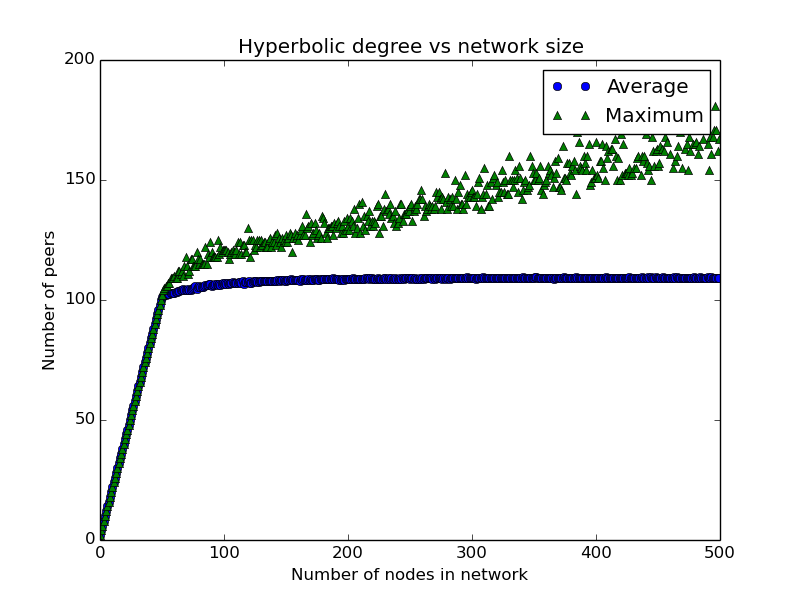
\includegraphics[width=\linewidth]{figs/HyperbolicDegree}
\caption{The Hyperbolic network uses the same long and short peer strategies to the Euclidean network, and thus shows similar results.}
\label{fig:HyperbolicDegree}
\end{figure}
\begin{figure}
\centering
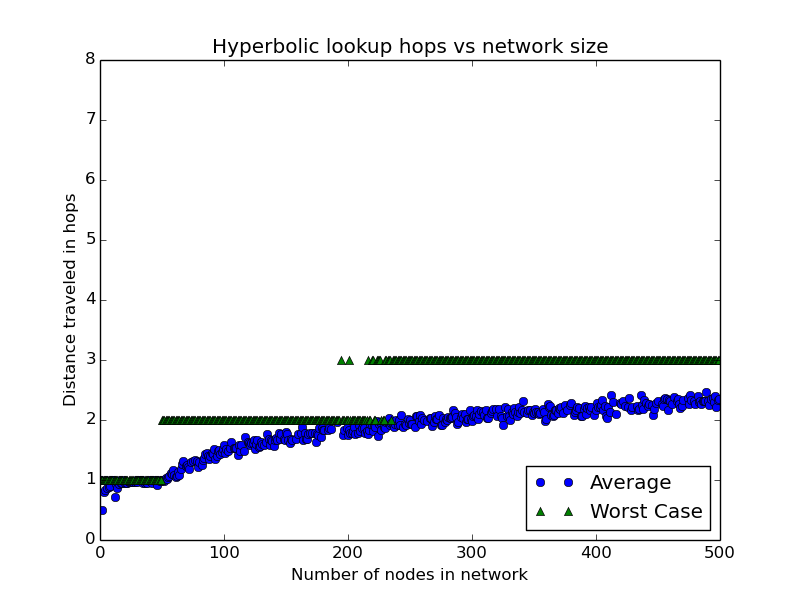
\includegraphics[width=\linewidth]{figs/HyperbolicDistance}
\caption{Like the Euclidean Geometry, our Poincar\`{e} disc based topology has much shorter maximum and average distances.
}
\label{fig:HyperbolicDistance}
\end{figure}


\section{Related Work}\label{sec:related}

There have been a number of efforts to either create abstractions of DHTs or ease the development of DHTs.
One area of previous work focused on constructing overlay networks using system called P2 \cite{p2} \cite{loo2005implementing}.
P2 is a network engine for constructing overlays which uses the Overlog declarative logic language.
Writing programs for P2 in Overlog yields extremely concise and modular implementations of for overlay networks. 

Our work differs in that P2 attempts to abstract overlays and ease construction by using a language and framework. while UrDHT focuses on abstracting the idea of a structured overlay into Voronoi Tessellations and Delaunay Triangulations.
This allows developers to define the overlays they are building by mathematically defining a short number of functions.

Our use case is also subtly different. 
P2 focuses on overlays in general, all types of overlays.
UrDHT concerns itself solely with distributed hash tables, specifically, overlays that rely on hash functions to distribute the load of the network and assign responsibility in an autonomous manner. 

One difficulty in using P2 is that it is no longer supported as a project \cite{p2}. 
P2's concise Overlog statements also present a sharp learning curve for many developers.
These present challenges not seen with UrDHT.


The T-Man\cite{jelasity2005t} and Vicinity \cite{voulgaris2005epidemic} protocols both present gossip-based methods for organizing overlay networks.
The idea behind T-Man is similar to UrDHT, but again it focuses on overlays in general, while UrDHT applies specifically to DHTs.
% T-man boasts the topology can change at run-time as the needs demand. 
The ranking function is similar to the metrics used by UrDHT using DGVH, but DGVH guarantees full connectivity in all cases and is based on the inherent relationship between Voronoi Tessellations, Delaunay Triangulations, and DHTs.

UrDHT uses a gossiping protocol similar to the ones presented by T-Man and Vicinity due to they gossip protocol's ability to rapidly adjust changes in the topology.


\section{Applications and Future Work}
\label{sec:future}

%Restate the intro
We presented UrDHT, a unified model for DHTs and framework for building distributed applications.
We have shown how it possible to use UrDHT to not only implement traditional DHTs such as Chord and Kademlia, but also in much more generalized spaces such as Euclidean and Hyperbolic geometries.
The viability of UrDHT to utilize Euclidean and Hyperbolic metric spaces indicates that further research into potential topologies of DHTs and potential applications of these topologies is warranted.


%Future improvements of UrDHT would further disconnect long peers and short peers giving them their own implementation cycle.

%Future stuff
There are numerous routes we can take with our model.
Of particular interest are the applications of building a DHT overlay that operates in a hyperbolic geometry.

One of the other features shared by nearly every DHT is that routing works by minimizing the number of hops across the overlay network, with all hops treated as the same length.
This is done because it is assumed that DHTs know nothing about the state of actual infrastructure the overlay is built upon.

However, this means that most DHTs could happily route a message from one continent to another and back.
This is obviously undesirable, but it is the status quo in DHTs.
The reason for this stems from the generation of node IDs in DHTs. 
Nodes are typically assigned a point in the range of a cryptographic hash function. 
The ID corresponds to the hash of some identifier or given a point randomly.
This is done for purposes of load balancing and fault tolerance.

For future work, we want to see if there is a means of embedding latency into the DHT, while still maintaining the system's fault tolerance.
Doing so would mean that the hops traversed to a destination are, in fact, the shortest path to the destination.

We believe we can embed a latency graph in a hyperbolic space and define UrDHT such that it operates within this space \cite{kleinberg2007geographic} \cite{cvetkovski2009hyperbolic}.
The end result would be a DHT with latency embedded into the overlay.
Nodes would respond to changes in latency and the network by rejoining the network at new positions.
This approach would maintain the decentralized strengths of DHTs, while reducing overall delay and communication costs.


\section{Remarks} % done
	\chapter{D$^{3}$DNS}
\label{chapter:d3ns}
	
%	We present D$^{3}$NS, a system to replace the current top level DNS system and certificate authorities, offering increased scalability, security and robustness. 
%	
%	D$^{3}$NS is based on a distributed hash table and utilizes a domain name ownership system based on the Bitcoin blockchain.  It addresses previous criticism that a DHT would not suffice as a DNS replacement. 
%	
%	D$^{3}$NS provides solutions to current DNS vulnerabilities such as DDOS attacks, DNS spoofing and censorship by local governments. D$^{3}$NS eliminates the need for certificate authorities by providing a decentralized authenticated record of domain name ownership. Unlike previous DNS replacement proposals, D$^{3}$NS is reverse compatible with DNS and allows for incremental implementation within the current system.
%	
	%We have created a system to replace the top level of the Domain Name system. The goal is to replace the top level of DNS with a network of authoratative name servers sharing their DNS records over a DHT.
	
	%We attempt to address the core problem posed by centralized trusted third parties. Specifically that centralized authorities are a single point of failure for trust. We seek to diffuse the responsibility of these system such that abuse of trust is more difficult.
	
	%It is reverse compatible with traditional DNS and entirely transparent to end users.
	


%\section{Introduction}
The Domain Name System, commonly referred to as DNS \cite{mockapetris2003rfc} \cite{mockapetris2004rfc}, is a fundamental component of the Internet.  DNS maps memorable names to the numerical IP addresses used by computers to communicate over IP. 

%cut this for conference?
Two recent events in the United states have brought DNS to the forefront of networking and security research.  First is recent legislation proposed in the US House of Representatives and US Senate. The Stop Online Piracy Act (SOPA) \cite{sopa} and PROTECT IP Act (PIPA) \cite{pipa} were both introduced in 2011.  There were numerous aspects to both bills, but essential to both was that DNS servers located in the US would be required filter DNS records on demand, essentially fracturing the DNS system.  There would be no guarantee that DNS could serve the same information to two different users.

More recent are the leaks of classified information elucidating the extent of the NSA's spying capabilities. These leaks have raised questions about the security of SSL and TLS, as well as the level of trust that users place in certificate authorities.


These types of threats to DNS, along with security concerns, were not considered when designing the protocol, but DNS is too widely used and too integrated with the Internet as a whole to be replaced. Extensions such as DNSSEC \cite{blacka2013clarifications} add authentication and data integrity, but do not alter the fundamental architecture of the DNS network.


There have been many explorations and attempts \cite{cox2002serving} \cite{pappas2006comparative} \cite{ramasubramanian2004design} to propose a DNS system based on a distributed hash table (DHT) \cite{chord}. We extend on those papers by implementing a DHT which minimizes latency distance rather than hop distance and implementing a shared record of ownership based on recent developments in cryptocurrency \cite{namecoin} \cite{bitcoin}.


This paper proposes the Distributed Decentralized Domain Name Service, or D$^{3}$NS.  D$^{3}$NS is a completely decentralized Domain Name Service operating over a DHT.  D$^{3}$NS does not replace the DNS protocol, but rather adds robustness to the architecture as a whole.  Internally, D$^3$NS signs all DNS records using public/private keys, providing additional security internal to the DNS system.

We show that D$^{3}$NS addresses the objections to a decentralized DNS system posed by Cox \textit{et al}. \cite{cox2002serving}, specifically: dramatically reducing latency compared to other DHT systems, retaining the extensibility of the original DNS system, and changing the intended scope of use to address incentive issues. We show D$^{3}$NS allows for new authentication methods and a means of decentralized proof of ownership beyond that of Cox \textit{et al}.'s work. 


The rest of the paper is consists of the following sections.  Section II gives an overview of DNS and identifies prior research in the area of distributed DNS.  Section III defines the various components of D$^3$NS.  Section IV covers the modified blockchain used for record authentication in D$^3$NS.  Section V presents UrDHT \cite{urdht}, a DHT that we designed and used with D$^3$NS.  Section VI details our implementation of D$^3$NS and  we discuss our conclusions and future work in Section VIII.


\section{Background}

This paper is intended to address concerns raised by Cox \textit{et al}. \cite{cox2002serving} and propose a viable decentralized DNS replacement utilizing a DHT. Our proposed improvements on the DNS alternative presented by Cox \textit{et al}. are fully reverse compatible with the current hierarchical DNS system and provides a shared, authenticated public record that allows for DNSSEC style authentication.

\subsection{DNS Overview}

DNS queries proceed recursively through the DNS hierarchy, beginning with a query to a root server, which then yields a record for a server for the requested top level domain.  This server then directs the request to another DNS server responsible for the domain under that, which yields an answer or another DNS server, which is queried in the same manner.

One of the key concepts of the DNS architecture is that no matter which servers end up being queried, a user can expect to receive a record consistent with what the rest of the DNS system will serve for that particular request.

Recent legislative motions reflect DNS's weakness to be influenced by local government intervention \cite{sopa} \cite{lemley2011don} \cite{crocker2011security}.

These bills would have required that servers maintained in the US filter specified domain names, preventing users from obtaining the correct IP address for the domain name in question. Multiple governments have been noted to preform systematic attacks on DNS queries \cite{inject}. This filtering is incompatible with the DNS Security Extensions (DNSSEC) \cite{crocker2011security} and DNS's intended usage. 

The mandated DNS filtering would possibly drive users to unregulated DNS servers, which would create more attack vectors.


\subsection{Related Work}
Cox \textit{et al}. devised a distributed DNS using Chord \cite{chord} as the storage medium for DNS records, which they called Distributed DNS (DDNS). They examined the possibility of extending DNSSEC with new options for storing keys in the DHT. They encountered the then unsolved problem of proof-of-ownership \cite{bitcoin} for domain names and found no means of enhancing security. 

They noted that the overlay topology of a DHT such as Chord did not take into account latency optimization and thus DNS was not a viable application of a DHT due to significantly greater latency. They also pointed out several possible improvements as a result of using a DHT, namely increased robustness, an auto-balancing structure, resistance to both DDOS attacks and packet injection based DNS spoofing.


Cox \textit{et al}. considered the optimization and security problems solvable, but they postulated that two issues rendered the system unviable. First, they intended that DDNS would replace all DNS servers and traffic, which removed extensibility and customizability of the original DNS protocol. Second, because they considered replacing the entire DNS system rather than a meaningful subset, they presented a question of incentive. What would incentivize companies to support the new system where their servers had to share the load of other companies traffic?  What would stop them from holding only their content, while rejecting any additional responsibility assigned to it?


D$^3$NS addresses both of the raised issues. 
We utilize a side channel method of confirming domain named ownership via a blockchain \cite{namecoin} to enable DNSSEC style security at all layers of the network. 
We propose a DHT structure which allows for minimum latency optimization. 
Our system aims only to replace authoritative Top Level Domain servers currently managed by registrars, where most records are simply a forward to an authoritative DNS server managed by the domain owner, rather than replacing all levels of DNS. 
This limiting of scope allows us to continue to take advantage of DNS extensions and as places responsibility of managing the network with those who have an incentive for its continued functioning.



\section{D$^{3}$NS}
D$^{3}$NS has logically discrete components which provide DNS efficient record storage, domain name ownership management and verification, and DNS backwards compatibility, all of which may be modularly replaced or have individual optimizations. 
D$^{3}$NS uses a DHT to store DNS records in a distributed fashion and a blockchain and Namecoin \cite{namecoin} analog to manage domain name ownership.  
D$^{3}$NS utilizes public and private key encryption for signing and verifying records.


\subsection{Distributed Hash Table}
Our implementation is not strictly specific to any particular distributed hash table.  We examined using Chord \cite{chord} with DNS, similar to DDNS \cite{cox2002serving}.  However, Chord's unidirectional ring overlay topology does not take actual network topology into account and using it for a global scale system is not viable because messages will be routed very inefficiently. D$^3$NS requires a DHT which allows the routing overlay to be optimized to the network topology and conditions in real time.


As a result we chose to develop a prototype DHT to meet this requirement to act as backend to our DNS system called UrDHT \cite{urdht}. 
UrDHT is built on the idea of constructing the DHTs overlay by using Voronoi Tessellations and Delaunay Triangulation. 
Essentially, each node is at the center of Voronoi region and responsible for the records that fall in that region.
The peers the node connects with correspond to that node's Delaunay neighbors. 
Because UrDHT works with the high level abstractions of Voronoi Tessellation and Delaunay Triangulation, UrDHT can  easily be configured to work in any arbitrary metric space or imitate the overlay topology of any DHT, such as Chord.

For D$^{3}$NS, UrDHT uses a $d$-dimensional unit cube which wraps around the edges in a toroidal fashion as the space for the overlay.
Each record in the DHT is assigned a location in that space. 
Each node is assigned a location and is responsible for records to which it is the closest node.
The variable dimensionality is allowed so that problems can be embedded into the space with relative ease and records can be assigned locations which have meaning concerning the problem in which they are a part. 
This way, records that are close to each other in the problem formulation are close to each other in the DHT and are likely hosted on the same node. 
This offers speedup for many distributed algorithms which require traversal of data.


\subsection{DNS Frontend}
Because this system is intended to be reverse compatible with the existing DNS protocol, we serve the data provided by the DHT after it has been authenticated by the block chain to other DNS servers or clients. DNS nodes incorporated into the D$^3$NS system will not request data from other DNS servers and will only exchange data via the DHT.


\section{Blockchain}
We use a tool called a \emph{blockchain} for maintaining and  authenticating our DNS records.  Blockchains have their roots in the cryptocurrency Bitcoin \cite{bitcoin}, where it is used to authenticate financial transactions and verify account balances.  While there have been similar attempts to leverage Bitcoin's mechanisms extend DNS \cite{namecoin}, they have been strictly tied to the concept of currency and not yet academically explored.

\subsection{Blockchains in Bitcoin}
Bitcoin is a decentralized electronic currency. 
Here we are particularly concerned with Bitcoin's blockchain. Bitcoin's blockchain consists of a shared authenticatable transaction record \cite{namecoin}  \cite{bitcoin} .


\begin{figure}
	\centering
	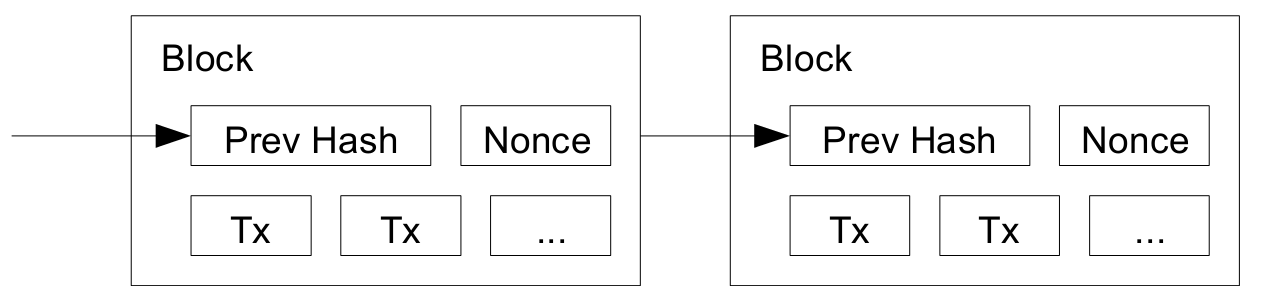
\includegraphics[width=0.7\linewidth]{figs/blockchain}
	\caption[A blockchain segment]{A section of the blockchain as defined by Bitcoin \cite{bitcoin}.}
	\label{fig:blockchain}
\end{figure}


Bitcoin's blockchain is essentially a shared ledger.  The blockchain (Figure \ref{fig:blockchain}) is a record of every single transaction made using the Bitcoin. Each transaction refers to  a previous transaction, indicating the funds handled by the new transaction are in fact owned by the user initiating the transaction. The record is validated by traversing the tree of transactions and marking the referenced transactions as used. A valid blockchain has all non-leaf node transactions marked as used only once.


Transactions are grouped together and verified in a \emph{block}, which are linked together in a chain.  Each block in the chain is a series of transactions published during the time it takes to generate that block. The process of authenticating these transactions and generating a new block is called mining (Algorithm \ref{alg:mining}).  Mining a block is analogous to the concept of gold mining, as the incentive for successfully mining a block is a large sum of new bitcoins.  

A block is mined by generating a nonce field such that the hash of the entire block is less than a global difficulty value. This difficulty sets the rate at which new blocks are mined and is adjusted in reference to rate of mining \footnote{Bitcoin adjusts the difficulty rate every 2016 blocks, such that the network will then mine a block every ten minutes on average \cite{bitdiff}}.  When a block is mined, it is transmitted to the network and each transaction in it is validated by each peer. The network will then work on mining the next block.

\begin{algorithm}
	\caption{Blockchain mining}
	\label{alg:mining}
	\begin{algorithmic}[1]  % the number is how many 
		\State Given previous Block $B_{-1}$
		\State Given New Transaction Set $T$
		\State Given Difficulty $D$
		\State Given Reward destination $R$
		\State New Block $B_0$ = $HASH(B_{-1})|T|R|Timestamp$
		\State Block Attempt $b$ = $B_0|Nonce$
		\While {$HASH(b) > D$}
			\State Block Attempt $b$ = $B_0|Nonce$
		\EndWhile
		\State Propagate $b$ as next block
	\end{algorithmic}
\end{algorithm}


\subsection{Using the Blockchain to validate DNS records}
We utilize the transaction record of Bitcoin to record ownership of domain names. Rather than rewarding miners with currency,  the reward and incentive for mining is a record that allots the miner the right to claim a domain name.  


\begin{algorithm}
	\caption{Blockchain Transaction Validation}
	\label{alg:validation}
	\begin{algorithmic}[1]  % the number is how many 
		\State A new transaction $t$ consists of: Award domain $D$ to user $U$ with proof reference $P$ and signature $S$
		\State The transaction set $T$ is the set of all transactions considered valid
		\If{$P$ is not marked used}
		\If{owner indicated in $P$ matches signature $S$}
		\If{$D$ matches domain referenced in $P$}
		\State Mark $P$ as used
		\State Consider $t$ valid
		\Else
		\If{$P$ is a mining reward}
		\State $P$ is an unclaimed mining reward
		\If{$D$ is not yet claimed}
		\State Mark $P$ as used
		\State  Mark $D$ as claimed
		\State Consider $t$ valid
		\EndIf
		\EndIf
		\EndIf
		\EndIf
		\EndIf
	\end{algorithmic}
\end{algorithm}

The transactions in each block indicate miners claiming a new domain or the transfer of domain ownership. Claims of new domains are validated by a reference to an unclaimed mining reward owned by the claiming user. Transfers are validated by a pointer to an unused previous transfer record or claim record indicating ownership by the transferring party. This way every domain name in the system can be associated with the owner's public key. New domains can be claimed and old domains can be transfered between owners.
Algorithm \ref{alg:validation} shows the process for validating transactions using the blockchain.







\subsection{Using a Blockchain to Replace Certificate Authority}
The shared record of the blockchain allows any participant in the mining network to act as a trusted third party to clients. This way, trust is not centralized at a single point of failure. 

Internally, members of the DHT are also members of the blockchain network (as it is convenient to use the DHT overlay as the Blockchain network overlay) and thus all records pushed to the DHT and retrieved records can be confirmed as legitimate before transmission to the end user. This limits the viability of replay or injection based attacks.




\section{UrDHT}
%VHash was created to allow for spacial representations to be mapped to hash locations, a feature lacking in many current distributed hash tables.  In particular, we aimed to construct a mechanism for creating a more efficient global scale DHT built on a minimal latency overlay. Rather than focus on minimizing the amount of hops required to travel from point to point we wish to minimize the time required for a message to reach its recipient. VHash actually has a worse worst case hop distance ($O(\sqrt[d]{n})$) than other comparable distributed hash tables ($O(lg(n))$). However, VHash can route messages as quickly as possible rather than traveling over a grand tour that an overlay network may describe in the real world.

One of the reasons we created UrDHT \cite{urdht} was to allow for spacial representations to be mapped to hash locations, a feature lacking in many current distributed hash tables.  
In particular, we aimed to construct a mechanism for creating a more efficient global scale DHT built on a minimal latency overlay. 
Rather than focus on minimizing the amount of hops required to travel from point to point we wish to minimize the time required for a message to reach its recipient. 
UrDHT actually has a worse worst-case hop distance ($O(\sqrt[d]{n})$) than other comparable distributed hash tables ($O(lg(n))$). 
However, UrDHT can route messages as quickly as possible rather than traveling over a grand tour that an overlay network may describe in the real world.



The naive method of doing so is to assign coordinates to servers based on the geographic location of nodes. More complex approaches would approximate a minimum latency space based on inter-node latency.
Algorithm \ref{alg:latency} describes the process for performing a minimum latency embedding using UrDHT

%The intent is that meaning can be ascribed to locations in the DHT and facilitate more efficent function. 
%Specifically in this example we seek to build a minimal latency overlay network for the DHT so a global scale DHT is viable and efficent. 








\begin{algorithm}
	\caption{UrDHT Minimum Latency Embedding}
	\label{alg:latency}
	\begin{algorithmic}[1]  % the number is how many 
		\State $d$ is the dimensions of the hash space
		\State seed the space with $d+1$ nodes at random locations
		\State A node $n$ wishes to join the network
		\State $n$ pings a random subset of peers to find latencies $L$
		\State Normalize $L$ onto (0.0,1.0) to yield $L_N$
		\State Choose position $p$ such that $$\sum\limits_{i\in peers}(L_N[i]-dist(p,i))^2$$ is minimized
		\State Re-evaluate location periodically
	\end{algorithmic}
\end{algorithm}







\subsection{Toroidal Distance Equation}

Given two vector locations $\vec{a}$ and $\vec{b}$ on a  $d$ dimensional unit toroidal hypercube:
\[ distance = \sqrt[|d|]{\sum\limits_{i\in d} (\min(|\vec{a}_i-\vec{b}_i|,1.0-|\vec{a}_i-\vec{b}_i|))^2}\]

\subsection{Mechanism}
UrDHT maps nodes to a $d$ dimension toroidal unit space overlay. This is essentially a hypercube with wrapping edges. The toroidal property makes visualization difficult but allows for a space without a sparse edge, as all nodes can translate the space such that they are at the center of the space.  In effect, each node views itself at the center of the graph.

Nodes in UrDHT are responsible for the address space defined by their Voronoi region. This region is defined by a list of peers maintained by the node. A minimum list of peers is maintained such that the node's Voronoi region is well defined. The links connecting the node to its peers correspond to the links of a Delaunay Triangulation.  One such possible network is shown on Figure \ref{fig:churninit}.


\begin{figure}
	\centering
	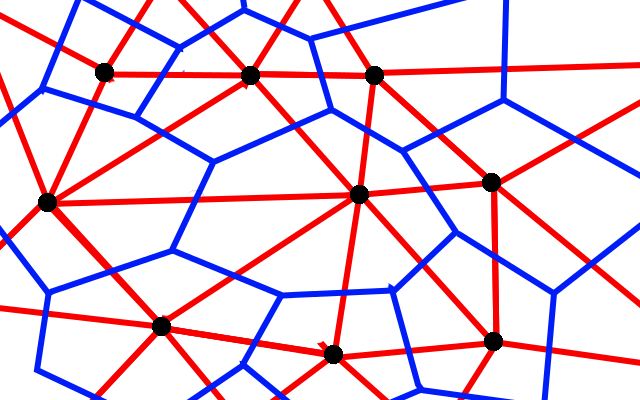
\includegraphics[width=0.5\linewidth]{figs/voronoi-churn2}
	\caption[The starting network topology]{The starting network topology.  The blue lines demarcate  the Voronoi edges, while the red lines connecting the nodes correspond to the Delaunay Triangulation edges and one-hop connections.}
	\label{fig:churninit}
\end{figure}

\subsection{Relation to Voronoi Diagrams and Delaunay Triangulation}

UrDHT does not strictly solve Voronoi diagrams \cite{voronoi} for a number of reasons. 
DHTs are completed decentralized, with no single node having global knowledge of the topology.
Many of the algorithms to compute Delaunay Triangulation and/or Voronoi Tessellation are unsuited to a distributed environment.
In addition, the computational cost increases when we move into spaces with greater than two dimensions.
In general, finding the Delaunay Triangulation of $n$ points in a space with $d$ dimensions takes $O(n^{\frac{2d-1}{d}})$ time \cite{watson1981computing}.

UrDHT uses the Distributed Greedy Voronoi Heuristic \cite{dgvh}, to create an approximation of Voronoi tessellation and Del. 
%Rather than attempt to calculate the Voronoi region of each node, it simply filters locations, assigning responsibility to the nearest node. 
An online algorithm (Algorithm \ref{alg:dgvh} maintains the set of peers defining the node's Voronoi region. The set of peers required to define a node's Voronoi Region corresponds to a solution to the dual Delaunay Triangulation.


%
%\begin{algorithm}
%	\caption{DGVH Greedy Peer Selection}
%	\label{alg:dgvh}
%	\begin{algorithmic}[1]  % the number is how many 
%		\STATE $Candidates$ is the set of candidate peers
%		\STATE $Peers$ is the set of this node's peers
%		\STATE $Candidates$ is sorted by each node's distance to this node
%		\STATE The closest member of $Candidates$ is popped and added to $Peers$
%		\FORALL{$n$ in $Canidates$}
%		\STATE $c$ is the midpoint between this node and $n$
%		\IF{Any node in $Peers$ is closer to $c$ than this node}
%		\STATE reject $n$ as a peer
%		\ELSE
%		\STATE Add $n$ to $Peers$
%		\ENDIF
%		\ENDFOR
%	\end{algorithmic}
%\end{algorithm}


\subsection{Messages}
Maintenance and joining are handled by a simple periodic mechanism. A notification message consisting of a node's information and active peers is the only maintenance message. All messages have a destination hash location which is used to route them to the proper server. This destination can be the hash location of a particular node or the location of a desired record or service.  The message is received by the node responsible for the location. Services running on the DHT define their own message contents, such as commands to store and retrieve data.

\subsection{Message Routing}
Messages are routed over the overlay network using a simple algorithm ( Algorithm \ref{alg:routing}). 
When routing a message to an arbitrary location, a node calculates which Voronoi region the message's destination is in amongst the itself and its peers. If the destination falls within its own region, then it is responsible and handles the message accordingly. Otherwise, the node forwards the message to the closest peer to the destination location. This process describes a precomputed and cached A* routing  algorithm \cite{astar} . 

%\begin{algorithm}
%	\caption{Routing}
%	\label{alg:routing}
%	\begin{algorithmic}[1]  % the number is how many 
%		\STATE $P_0$ is this node's set of peers
%		\STATE $N$ is this node
%		\STATE $m$ is a message addressed for $L$
%		\STATE $Forwards$ is the set $P_0\cup{}N$
%		\STATE find $C$: member of $Forwards$ which has the shortest distance to $L$
%		\IF{$C$ is $N$}
%		\STATE $N$ is the responsible party.
%		\STATE Handle $m$
%		\ELSE
%		\STATE Forward $m$ to $C$ for handling or further routing
%		\ENDIF
%	\end{algorithmic}
%\end{algorithm}

\subsection{Joining and Maintenance}
Joining the network is a straightforward process. A new node first learns the location of at least one member of the network to join. The joining node then choses a location in the hash space either at random or based on a problem formulation (for example, based on geographic location or latency information).

After choosing a location, the joining node sends a \textit{join} message to its own location via the known node.
The message is forwarded to the current owner of that location who can be considered the ``parent'' node.
The parent node immediately replies with a maintenance message containing its full peer list. 
This message is sent to the joining node, who then uses this to begin defining the space it is responsible for. 

The joining node's initial peers are a subset of the parent and the parent's peers. The parent adds the new node to its own peer list and removes all his peers occluded by the new node.  Then regular maintenance propagates the new node's information and repairs the overlay topology.  This process is described by Algorithm \ref{alg:join}.


%TODO Move to DGVH or UrDHT
\begin{algorithm}
	\caption{Join}
	\label{alg:join}
	\begin{algorithmic}[1]  % the number is how many 
		\State new node $N$ wishes to join and has location $L$
		\State  $N$ knows node $x$ to be a member of the network
		\State  $N$ sends a request to join, addressed to $L$ via $x$
		\State  node $Parent$ is responsible for location $L$ and receives the join message
		\State  $Parent$ sends to $N$ its own location and list of peers
		\State  $Parent$ integrates $N$ into its peer set
		\State  $N$ builds its peer list from $N$ and its peers
		\State regular maintenance updates other peers
	\end{algorithmic}
\end{algorithm}


Each node in the network performs maintenance periodically by a maintenance message to its peers. The maintenance message consists of the node's information and the information on that node's peer list. When a maintenance message is received, the receiving node considers the listed nodes as candidates for its own peer list and removes any occluded nodes (Algorithm \ref{alg:dgvh}). 




When messages sent to a peer fail, it is assumed the peer has left the network. The leaving peer is removed from the peer list and candidates from the set of 2-hop peers provided by other peers move in to replace it.  Maintenance is described by Algorithms \ref{alg:maint} and \ref{alg:handlemaint}.  Figures \ref{fig:churnjoin}, \ref{fig:churndone}, and \ref{fig:churndrop} illustrate the joining processing.

\begin{algorithm}
	\caption{Maintenance Cycle}
	\label{alg:maint}
	\begin{algorithmic}[1]  % the number is how many 
		\State $P_0$ is this node's set of peers
		\State $T$ is the maintenance period
		\While{Node is running}
		\ForAll{node $n$ in $P_0$}
		\State Send a Maintenance Message containing $P_0$ to $n$
		\EndFor
		\State Wait $T$ seconds
		\EndWhile
	\end{algorithmic}
\end{algorithm}


\begin{algorithm}
	\caption{Handle Maintenance Message}
	\label{alg:handlemaint}
	\begin{algorithmic}[1]  % the number is how many 
		\State $P_0$ is this node's set of peers
		\State Receive a Maintenance Message from peer $n$ containing its set of peers:$P_n$
		\ForAll{Peers $p$ in $P_n$}
		\State Consider $p$ as a member of $P_0$
		\If{$p$ should join $P_0$}
		\State Add $p$ to $P_0$
		\ForAll {Other peers $i$ in $p$}
		\If{$i$ is occluded by $p$}
		\State remove $i$ from $P_0$
		\EndIf
		\EndFor
		\EndIf
		\EndFor
	\end{algorithmic}
\end{algorithm}




There is no function for a ``polite'' exit from the network. UrDHT assumes nodes will fail and the difference between an intended failure and unintended failure is unnecessary. The only issue this causes is that node software should be designed to fail totally when issues arise rather then attempt to fulfill only part of its responsibilities.  





\begin{figure}
	\centering
	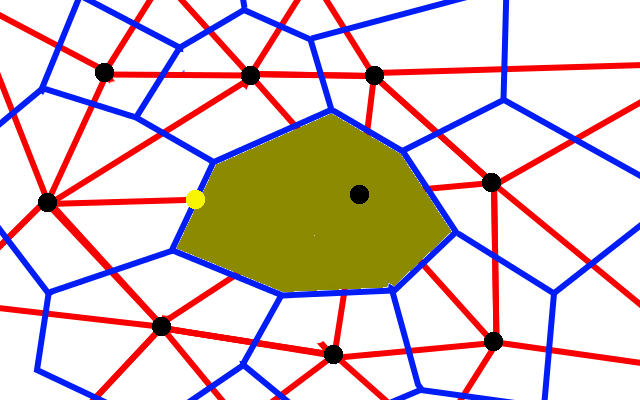
\includegraphics[width=0.5\linewidth]{figs/voronoi-churn4}
	\caption[Topology before join]{Here, a new node is joining the networks and has established that his position falls in the the yellow shaded Voronoi region.}
	\label{fig:churnjoin}
\end{figure}


\begin{figure}
	\centering
	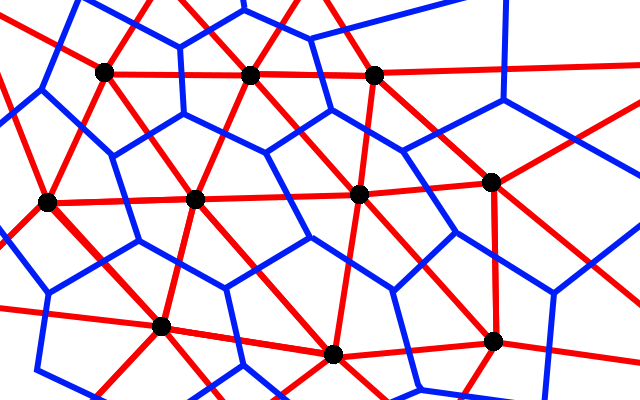
\includegraphics[width=0.5\linewidth]{figs/voronoi-example}
	\caption[Topology after join]{The network topology after the new node has finished joining.}
	\label{fig:churndone}
\end{figure}

\begin{figure}
	\centering
	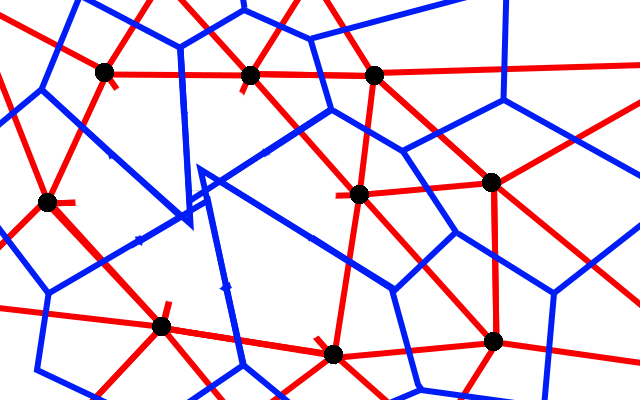
\includegraphics[width=0.5\linewidth]{figs/voronoi-churn1}
	\caption[Topology after failure]{The topology immediately after the new node leaves the network. After maintenance takes place, the topology repairs itself back to the configuration shown in Figure \ref{fig:churninit}.}
	\label{fig:churndrop}
\end{figure}


\subsection{Data Storage and Backups}
The primary goal of a DHT is to provide a distributed storage medium. We extend this idea to distribute work and information among nodes using the same paradigm. Resources in the network, be it raw data or assigned tasks, are assigned hash locations. The node responsible for a given hash location is responsible for the maintenance of that resource. When a node fails, its peers take responsibility of its space. Thus it is important to provide peers with frequent backups of a node's assigned resources.  That way, when a node fails, its peers can immediately assume its responsibilities.

When a resource is to be stored on the network, it is assigned a hash location. The hash locations assigned could be random, a hash of an identifier, or have specific meaning for an embedding problem. The node responsible for that resource's hash location stores the resource.

A resource is accessed by contacting the node responsible for the resource.  However, the requester generally has no idea which node is responsible for any particular resource.  The data request messsage is addressed to the location corresponding to the resource, rather than the node responsible for that location.  The message is forwarded over the overlay network, each hop bringing the node closer until it reaches the responsible node, who sends the resource or an error if the resource does not exist.

Some options are immediately apparent for dealing with wasted storage space. A system that is primarily read driven can record the time of the last read or a frequency of reads such that resources that are not read often enough are deleted after a certain period of time. If a system is write driven, allow the resource to be assigned a time to live, which can be updated as needed.

A node periodically sends a message containing backups of the resources for which it became newly responsible for to each of its peers. To minimize bandwidth and time wasted by backups, the node should only send the records changed since last backup.



\section{Implementation}
This section describes how the components of the D$^3$NS system piece together as a coherent whole.  We demonstrate how this system would be used in the real world to provide a better Domain Name Service.


\subsection{Establishment of a New Domain}
Under the current DNS system, a new domain name is purchased from a company registered with the Internet Corporation for Assigned Names and Numbers (ICANN). That company adds the domain name and a record provided by the owner to the TLD servers. The owner or management company then maintains a name server to answer DNS requests for the purchased domain. In D$^{3}$NS, new domain names are instead awarded as part of the blockchain mining process or purchased from a previous owner, then transferred to the new owner. These assignments and transfers are both recorded in the blockchain. 

A prospective domain owner can use their own mining software and mine a domain name or purchase a domain name voucher from a miner and exchange it for a domain name. In the blockchain, domain name owners are referred to by their public key. The public key is used to authenticate both records and transfers of domains. Loss of the private key of an account will result in the loss of ability to update DNS records and the ability to transfer the domain. 


\subsection{Updating Records for a Domain}
A domain name record in the current DNS system is used to indicate a record on your own Name Server or to configure the record held by the TLD server that contains the address record. Using D$^3$NS, all records must be signed using their owner's private key and confirmed with the public key. 

A properly configured D$^3$NS server should not accept any DNS records which have not been signed by their owner or accept a record with an older version number. To push a new DNS record for a domain, the owner must create the record set for the domain and then sign and submit it to a node on the DHT. The DHT will forward the record to the responsible party and store it after confirming its validation. The new record will begin to be broadcast to clients after old records begin to expire and caches seek new records.

\subsection{Looking up a DNS record}
In the current DNS configuration, a record is looked up using a UDP system that queries a tree of servers. clients send queries to  a local DNS server which acts as a DNS resolver and cache. If a portion of the domain name is unknown, the resolver sends a request to the responsible server and looks the record up recursively.

This system is largely unchanged under D$^{3}$NS from the point of view of the DNS resolver and client. Ideally, the resolver or client has chosen a nearby member of the D$^{3}$NS network as its root domain name server (it can also maintain a large list of backup servers, should the current one fail). The resolver requests a domain's record from the D$^{3}$NS node. The node then forwards the request to the responsible party. If any node along the route has a valid cache of the required record, then that server responds and routes the message back to the entry node. All nodes along the route cache the response to aid future queries.

\subsection{Caching}
DNS needs to aggressively cache lookups. Previous investigations into optimizing caching on a DHT saw favorable results \cite{irm}. However, with the specific application of DNS in mind, the time-to-live field on DNS records defer the caching optimization problem onto users. 
While it may be tempting to utilize the built in time-to-live field for caching on the DHT, the possible cyclical nature of cache passing may result in difficulty in propagating new records.


Integrated File Replication and Consistency Maintenance (IRM) \cite{irm} views the process of caching and keeping the cache up to date as components of larger problem.  Nodes in the DHT keep track of how often records are requested and cache those records once a defined rate is passed.  Nodes then request an update for the cache based on how often the record is requested and how often that request is expected to be changed by the owner.


In the current implementation of DNS, caching involves a time-to-live field defined by the domain owner. This means that no effective cache optimization done by the server; rather the server that trusts records to have a sensible time-to-live value. IRM \cite{irm} can be used to approximate the correct time-to-live value for a record.

\section{Conclusion and Future Work}
D$^3$NS was successfully implemented to act as a DNS server.  A user would query the a computer we set up as a DNS gateway which was a member of the DHT and mining network. If the queried domain had a record stored in the DHT and an owner established in the blockchain, the server would reply with the stored DNS records. Otherwise the server would reply with a DNS failure. We ran the DHT and mining network on a cluster of computers and an artificially low difficulty such that a live demo of mining would be viable.

Using all of these components together allowed us to create a system with the following features:
\begin{itemize}
	\item Robustness - The DHT and Blockchain are both robust to failures and attacks.
	\item Extensibility - The DNS reverse compatibility allows any DNS extension to be utilized, if dynamic resolution is required a name server record can be stored in the DHT to point to a user's specialized DNS servers.
	\item Decentralization - Both the DHT and Blockchain can operate without the support of any controlling organization, this offers security against corruption and abuse. 
\end{itemize}	

D$^3$NS successfully addresses the challenges laid down by Cox \textit{et al}. \cite{cox2002serving}  in regards to designing a DNS replacement running over a DHT.   We encourage criticism, revision, and adoption of this new system.

\subsection{Unaddressed Issues and Future Work}
The Blockchain does not solve all security issues relevant to DNS authentication and security. Exit nodes could lie or have packets inject to clients until the protocol from DNS server to client is improved. The DHT structure opens up unexplored disruption attacks on the overlay topology.

A series of issues relevant to UrDHT are not addressed here due to limiting of scope, space, time, and a lack of actual solutions to the problems: The exact method of caching to optimize lookup time under real world usage. The overlay network being mapped onto latency results in nodes whose failure due to natural disaster to be comorbid with it's neighbors resulting to data loss. Comorbidity could be counteracted by more complex backup schemes.

Future work will explore various solutions to theses issues, as well as generalized improvements to D$^3$NS as whole.  In particular, the technique of allying a DHT value store for real-time data and a Blockchain for ownership verification may prove a viable technique for decentralizing other web services and enabling new shared storage and computation mediums.

However, D$^3$NS served as our first real application built with the concepts of DGVH, VHash, and UrDHT.
It served as a successful prototype for and demonstrated the viability of those ideas.

	\chapter{Analysis of The Sybil Attack}
\label{chapter:sybil}




\section{Introduction}
One of the key properties of structured peer-to-peer (P2P) systems is the lack of a centralized coordinator or authority.
P2P systems remove the vulnerability of a single point of failure and the susceptibility to a denial of service attack \cite{sybil}, but in doing so, open themselves up to new attacks.

Completely decentralized P2P systems are vulnerable to \textit{Eclipse attacks}, whereby an attacker completely occludes healthy nodes from one another.
This prevents them from communicating without being intercepted by the adversary.
Once an Eclipse attack has taken place, the adversary can launch a variety of crippling attacks, such as incorrectly routing messages or returning malicious data \cite{srivatsa2004vulnerabilities}.

One way to accomplish an Eclipse attack is to perform a \emph{Sybil attack} \cite{sybil}.
In a Sybil attack, the attacker masquerades as multiple nodes, effectively over-representing the attacker's presence in the network to maximize the number of links that can be established with healthy nodes.
If enough malicious nodes are injected into the system, the majority of the nodes will be occluded from one another, successfully performing an Eclipse attack.

This vulnerability is well known in the security community \cite{dhtsec}. 
Extensive research has been done assessing the damage an attacker can do after establishing themselves \cite{srivatsa2004vulnerabilities}.
%Especially when a hash value to assign neighbors
Little focus has been done on examining how the attacker can establish himself in the first place and precisely how easily the Sybil attack can be accomplished.


A simple method to generate node locations is to assign them at random.
A Sybil attack against this method is fairly straightforward; the attacker just assigns their own nodes at ``random'' locations.
A more sophisticated method to generate node locations would use a hash function of some unique characteristic of the node.
For example, a Distributed Hash Table could use a hash of the node's IP address and port number.
In this paper, we show that using a hash function provides no protection against a Sybil attack.

Our goal is to look at the Sybil attack from the perspective of an adversary executing the Sybil attack.
We did a formal analysis on the breadth and depth of the presence an adversary could establish on a structured P2P network.
%We also constructed simulations showing how an attacker could insert themselves into the network and proceed to incrementally inject malicious nodes in between normal members of the network, a process we call \textit{mashing}.
We also constructed simulations demonstrating the steps an attacker could follow to perform a Sybil attack.
Once the attacker has joined the network, they can proceed to incrementally inject malicious nodes directly in between members of the network, a process we call \textit{mashing}.

%Why am I doing this?
Sybil attacks represent a significant threat to the security of any distributed system.
Many of the analyses on Tor \cite{dingledine2004tor} emphasize the vulnerability of Tor to the Sybil attack \cite{bauer2007low}.
This threatens the anonymity of Tor users.

Sybil attacks are also a threat to P2P systems such as BitTorrent, which is essential to a wide variety of users.
BitTorrent is currently the \textit{de facto} platform for distributing large files scalably among tens of thousands of clients.
Many implementations rely on Mainline DHT (MLDHT) \cite{mainline} to connect users to other peers.
The number of users on Mainline DHT ranges from 15 million to 27 million users daily, with a turnover of 10 million users a day \cite{mainlineMeasure}.
Current research demonstrates BitTorrent is vulnerable to Sybil attacks and a persistent attack disabling BitTorrent would be highly detrimental to many users, especially developers and system administrators \cite{izal2004dissecting}.
BitTorrent is currently under an active Sybil attack \cite{sybilbit}, although the attackers are apparently not trying to destroy the network.

There have been many suggestions on how to defend against Sybil attack, but there is no agreed upon ``silver bullet'' among researchers that should be implemented for every distributed application \cite{levine2006survey} \cite{dhtsec}.
Urdaneta \textit{et al} find that in DHT security, a centralized, trusted authority which certifies or binds identities is the most effective strategy \cite{dhtsec}.
This solution potentially removes the Sybil attack, but reintroduces vulnerabilities to denial of service attacks and is contrary to the objective of creating fully decentralized systems.
Other techniques such as proof-of-work \cite{4215910} may provide a defense against Sybil attacks, but proof-of-work systems must set their computational puzzles to be simple enough for the weakest member of the network to participate.
However, the attacker can reasonably obtain computational power that is orders of magnitude greater than those weakest nodes and overcome the puzzle with brute force \cite{dhtsec}.

%Despite the threat represented by the Sybil attack and the research done on the subject, little research has been done from the perspective of an adversary.
%We sought to rectify this, both to reemphasize the threat of the Sybil attack, but also because this examination introduces some interesting graph theory problems.

Our work presents the following contributions:
\begin{itemize}
	%cut some?
	\item We first discuss the assumptions behind performing a Sybil attack on a structured P2P network and analyze how effective a Sybil attack is based on the resources available to the attacker.
	We show that in a size $n$ network being attacked by an adversary with $s$ distinct identities that the probability that \textit{any} given link leads to a Sybil is $P_{bad\_neighbor} =  \frac{s}{s+ n - 1}$ (Section \ref{sec:analysis}). 
	\item We present our simulations that show how quickly even a naive Sybil attack can compromise a system. 
	We validate our experimental results by comparing them with the equations we specify in our analysis (Section \ref{sec:sybil-sim}).
	%\item We analyze an interesting graph coloring problem that an attacker needs to solve if the attack is to remain undetected.
	\item We discuss the broader implications of our work, including how mashing can be used for automatic load balancing and disrupting P2P botnets (Section \ref{sec:horror}).
\end{itemize}

\section{Analysis}
\label{sec:analysis}

We make a few assumptions for our analysis; some apply to the P2P network we are analyzing and some create rules that restrict the adversary.
Without these assumptions, the Sybil attack becomes trivial to perform.


\subsection{Assumptions}
\label{sec:assume}

Our first assumption is that the systems we analyze are fully distributed and assign identities to nodes and data using a cryptographic hash function.
These systems are called distributed hash tables (DHTs).

Cryptographic hash functions work by mapping some input value to an $m$-bit key or identifier.
Well-known hash functions for performing this task include MD5 \cite{md5} and SHA1 \cite{sha1}.
Keys generated by the hash function in our analysis are assumed to be uniformly distributed and random \cite{bellare2004hash}, which we will see in the next chapter is not completely true. 
These hash functions are designed to make the intentional  discovery of collisions computationally difficult.

In distributed hash tables, $m$ is a large value in order to avoid collisions between mapped inputs, unintentional or otherwise. 
An $m \geq 128$ is typical, with $m = 160$ being the most popular choice.

Our second assumption is that node IDs are generated by hashing their IP address and port.
If the choice of ports are restricted, the attacker would have to obtain more IP addresses.
This is a form of very weak security that binds a particular hash key to a specific IP/port combination \cite{dinger2006defending} \cite{sit2002security}.
This method is often used as a means of generating node IDs.


Although other methods do exist, the only other one that is mentioned as often is to let nodes choose their own $m$-bit ID at random.\footnote{Another commonly mentioned method is hash public keys  \cite{dhtsec} \cite{sit2002security} \cite{pastry} \cite{castro2002secure}.  If the keys are certified or signed by an centralized source, we no longer have a completely decentralized network.  If the nodes are generating the keys themselves, then we have essentially the same problem as letting nodes choose keys at random.}
This is notably done in Mainline DHT, and makes the system extremely vulnerable to a Sybil attack.
Since there is no way to verify that a node chose the $m$-bit ID at random, nodes in the network accept advertised keys at face value.
This allows a prospective attacker to choose any specific key they want.

We also assume that nodes verify that a peer's advertised IP/port combination exists and that the hash function of these IP/port generates the correct node ID.
This verification is not explicitly used or implemented in any DHT. 
Failure to validate advertised values results in a trivial security flaw.
%Without it, our assumption about binding IDs to IP addresses and ports would be moot.

%Our final assumption is that the protocols being implemented by the network are secure and cannot be exploited by the attacker.


Consider an attacker operating under these assumptions who wants to inject a malicious node in between two victims which have no other nodes in between them.
The attacker must search for a valid IP and port combination under their control that generates a hash key that lies between the two victims' ID, a process we call \textit{mashing}.
The attacker's ability to compromise the network depends on what IP addresses and ports are available.

The process for mashing is similar to searching for a hash collision, but much easier.
Rather than searching for two inputs to a function that produce the same $m$-bit output, the attacker searches for a single input and corresponding $m$-bit hash that falls between two given $m$-bit IDs.
We assume the IDs are evenly distributed \cite{bellare2004hash}, so in a size $n$ network there would be $\approx \frac{2^{m}}{n}$ unused IDs between each pair of nodes.
This means the attacker is actually searching for a collision with one of $\approx \frac{2^{m}}{n}$ $m$-bit hashes, which is a much simpler problem.
%We would expect there to be a $50\%$ chance of a collision in a network with 

\subsection{Analysis}


Suppose we have a DHT with $n$ members in it, with $m$-bit node IDs between $[0,2^{m})$. 
Consider two victim nodes with IDs $a$ and $b$, with no others nodes with an ID in the range $(a,b)$.
%rwh a step that may make this clearer

The probability that a single mash key lies in the range of $(a,b)$ is $\frac{|b-a|}{2^{m}}$, which is the fraction of the network that lies between $ a $ and $ b $.
Thus the probability that the mash key does not lie in that range is $1-\frac{|b-a|}{2^{m}}$. 
Assuming that the individual mash keys are statistically independent yields the expression: $$(1-\frac{|b-a|}{2^{m}})^{num\_ips \cdot num\_ports} $$ for the probability that no mash key lands in the range.
%end of rwh insert  The changed to Thus The

Thus the probability $P$ that an attacker can mash a hash key that lands in the range $(a,b)$ is:
$$ P \approx 1 - (1 - \frac{|b-a|}{2^{m}})^{num\_ips \cdot num\_ports  } $$

where $num\_ip$ is the number of IP addresses the attacker has under thier control and $num\_ports$ is the number of ports the attacker can try for each IP address.


If the ports the attacker can utilize are limited to the ephemeral ports,\footnote{Also known as private or dynamic ports.  These ports are never assigned a specific use by the Internet Assigned Numbers Authority  and are available for applications to use as needed \cite{cotton2011internet}.} the attacker has 16383 ports to use for each IP address.
As previously noted, we assume that for a large enough $n$, node IDs will be close to evenly distributed across the keyspace.
This means $|b-a| \approx \frac{2^{m}}{n}$.
Therefore, the earlier probability is equivalent to:
$$ P \approx  1 - (1 -\frac{1}{n})^{num\_ips \cdot num\_ports}  $$
This indicates that the statistical ease of mashing is independent of $m$.

Given a healthy node, the probability $P_{bad\_neighbor}$ that a Sybil is its closest neighbor is:
\begin{equation}
P_{bad\_neighbor} =  \frac{num\_ips \cdot num\_ports}{num\_ips \cdot num\_ports + n - 1}
\label{eq:bad}
\end{equation}
This is effectively the number of malicous identities in the network ($num\_ips \cdot num\_ports$) over the total number of identities in the network.
Our experiments in Section \ref{sec:chord} show that $P_{bad\_neighbor}$ is actually the probability that \textit{any} of a nodes links connect to a Sybil.

From the previous equation, the adversary can compute how many unique IP/port combinations they need if they wish to obtain a desired probability $P_{bad\_neighbor}$:

$$ num\_ips \cdot num\_ports = P_{bad\_neighbor} \cdot \frac{n - 1}{1 - P_{bad\_neighbor} }$$

Using our previous assumption that the adversary is limited to the 16383 ephemeral ports, the attacker can computer the number of unique IP addresses needed:
$$ num\_ips  =  P_{bad\_neighbor} \cdot \frac{n - 1}{1 - P_{bad\_neighbor} }  \cdot \frac{1}{16383}$$


We verify these equations with our simulations.

\section{Simulations}
\label{sec:sybil-sim}
An essential part of our analysis was demonstrating just how fast an adversary can compromise a system.
We performed four experiments to accomplish this task.
These experiments were designed to analyze increasing levels of difficulty.
The first experiment demonstrates a hash attack is possible and later experiments verify the feasibility on larger and more complicated networks.
Our simulations were written in Python 2.7 and performed on an AMD Phenom II 965 processor. %, which had been overclocked to run at 3.7 GHz.

We used SHA1 as our cryptographic function, which yields 160-bit hash keys.
Again, we use the constraint that victim nodes do an absolute minimum verification which forces an attacker to only present Sybils with hash keys that they can generate with valid IP and port combinations.


%WE ASSUME THERE'S NO RESOURCE LIMITATIONS ON THE ATTACKER's end and this is reasonable because points below

We assume that the attacker has no resource limitations.
Previous research \cite{sybilbit} shows that an adversary performing a Sybil attack does not need to maintain the state information of other nodes and can leverage the healthy nodes to perform any needed routing.
Nor does the adversary necessarily need to create a new running copy for every Sybil created, but doing so is quite feasible. 
%If this was impossible, it is still reasonable to assume the attacker's program would be built to have a minimal memory footprint and drop any messages that require an attacker carry any of the network's load.


%Any application built using a DHT must be address its vulnerabilities to the Eclipse and Sybil attacks

%Security is not something that is thought about for a DHT, unless the 
%DHT is specifically made to be secure against X.  
%Or it's left to the applications



\subsection{Experiment 0: Mashing 2 random nodes}
Our initial experiment was designed to establish the feasibility of joining the network in between two random nodes.
Each trial, we generated two victims with random IP addresses and ports, and an attacker with a random IP address.
The experiment was for the attacker to find a key in between the two victims' keys, going clockwise.
The average amount of time over 10,000 trials to mash two random keys was 29.6218 microseconds, and was achievable $ 99.996\%$ of the time.

This test shows that the hashing operation is extremely quick.
However, two arbitrary nodes in a network can be and often are quite distant, in which case the mashing can be done quickly.
Our next experiment studies a more realistic condition.


\subsection{Experiment 1:  Time Needed to Mash a Region}
\label{sec:exp1}
After showing that mashing two arbitrary nodes takes a minuscule amount of time, the next step is to demonstrate that mashing the region between two adjacent nodes in a network of size $n$ also takes an inconsequential amount of time.
We simulate this by creating a sorted list of node IDs for $n$ random IP/port combinations and pick a random adjacent pair of numbers from the list.
The adversary then hashes their IP with their ports until they find an IP/port combination that results in a hash key falling in between the given pair.
Our results averaged 100 trials for each network size are shown in Figure \ref{fig:exp1} and Table \ref{tab:exp1}.

\begin{figure}
	\centering
	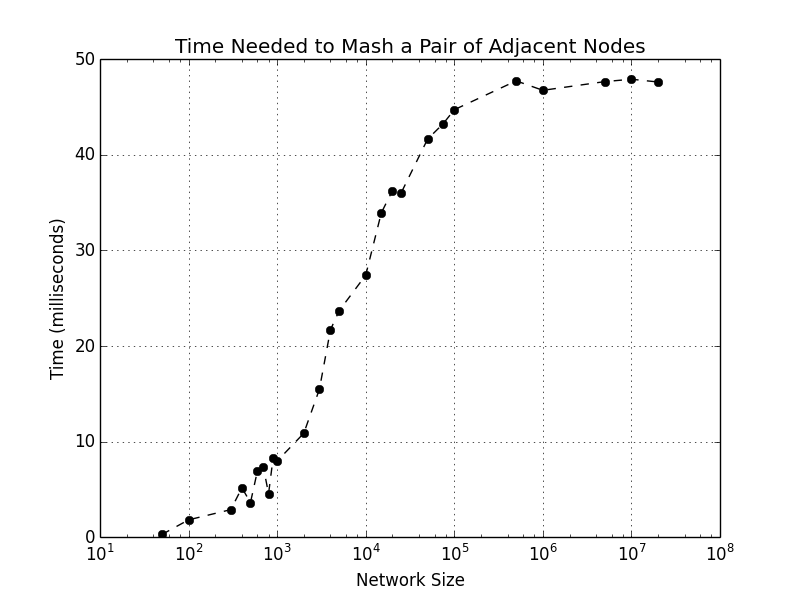
\includegraphics[width=\linewidth]{figs/size_time}
	\caption{This figure shows the amount of time needed for an adversary with a single IP address to mash a pair of adjacent nodes.  The time it takes to mash a pair of nodes begins to markedly increase once the network size gets above 1000 until it asymptotes at 48 ms.  For larger networks, more IP addresses are needed and precomputing becomes necessary.}
	\label{fig:exp1}
\end{figure}


\begin{table}\small
	\centering
	\caption{Times and success rate for mashing adjacent nodes for a single IP.}
	\label{tab:exp1}
	\begin{tabular}{|r|r|r|}
		\hline
		Network Size &  Success Rate &  Avg Time to Mash (ms) \\ \hline
		50 & 1.0 & 0.29 \\ \hline
		100 & 1.0 & 1.82 \\ \hline
		300 & 0.99 & 2.89 \\ \hline
		400 & 0.98 & 5.16999 \\ \hline
		500 & 1.0 & 3.62999 \\ \hline
		600 & 0.98 & 6.97 \\ \hline
		700 & 0.94 & 7.32 \\ \hline
		800 & 0.99 & 4.54999 \\ \hline
		900 & 0.92 & 8.28 \\ \hline
		1000 & 0.92 & 7.96999 \\ \hline
		2000 & 0.95 & 10.88 \\ \hline
		3000 & 0.88 & 15.47999 \\ \hline
		4000 & 0.74 & 21.7 \\ \hline
		5000 & 0.71 & 23.68 \\ \hline
		10000 & 0.67 & 27.41 \\ \hline
		15000 & 0.5 & 33.93 \\ \hline
		20000 & 0.37 & 36.24999 \\ \hline
		25000 & 0.39 & 35.98 \\ \hline
		50000 & 0.23 & 41.64999 \\ \hline
		75000 & 0.2 & 43.25999 \\ \hline
		100000 & 0.13 & 44.71999 \\ \hline
		500000 & 0.04 & 47.73999 \\ \hline
		1000000 & 0.03 & 46.75 \\ \hline
		5000000 & 0.0 & 47.65999 \\ \hline
		10000000 & 0.0 & 47.90999 \\ \hline
		20000000 & 0.0 & 47.62 \\ \hline
		
	\end{tabular}
\end{table}
These figures show that the larger the network size, the longer it takes for the adversary to mash a given pair of adjacent nodes.
Eventually, the time it takes to mash a region asymptotes to about 48 milliseconds.
This is the amount of time it takes for the adversary with a single IP to generate all 16383 hash combinations.
While this is a short time to mash a single region, an adversary following the attack specified in our next experiment will want to mash $n-1$ regions.
If the network size is 1 million, this process can take upwards of 13 hours in computational time.

Since the attacker's IP addresses and ports do not change over the course of the attack, the attacker would waste time by generating the same keys over and over. 
The mashing process could also take substantially longer if the network a hash function that produces numbers larger than 160 bits or if the network uses a more expensive function such as scrypt \cite{scrypt}.

The attacker can instead perform all the work needed to mash a network upfront, precomputing all possible valid hash keys.
We have shown this takes about 48 milliseconds for 16383 keys.
Storing these values in a sorted list costs 160 bits for each SHA1 key and 16 bits for each port, for a total of $176  \cdot 16383 = 2,883,408$ bits, or roughly 352 kilobytes for each IP address the attacker has.\footnote{Storing the IP address is unnecessary since it is always the same.}




%check chord coverage just with the successors
\subsection{Experiment 2:  Nearest Neighbor Eclipse via Sybil} %formerly 2
\label{sec:exp2}
The objective of this experiment is to completely eclipse a network using a Sybil attack, starting with a single malicious node.
We simulate this by creating a network of $n$ nodes.
Each node is represented by a key generated by taking the SHA1 of a random IP/port combination.

The goal of the attacker is to mash as many pairs of adjacent nodes as possible.
We call this the \textit{Nearest Neighbor Eclipse} since the attacker seeks to become the nearest neighbors of each node.

The attacker is given $num\_ips$ randomly generated IP addresses, but can use any port between 49152 and 65535.
This gives the attacker $ 16383 \cdot num\_ips $ possible hash keys to use for Sybils.
As mentioned previously in Section \ref{sec:exp1}, the attacker can easily precompute all of theses hash keys and store them in a sorted list to be used as needed, requiring only 352 kilobytes per IP.
Since this list is sorted and this attack will go in order through the network, searching for a key that mashes a pair of nodes takes constant time.

To perform the attack, an adversary choses any random hash key as a starting point to ``join'' the network.
This is their first Sybil and the join process provides information about a number of other nodes.
Most importantly, nodes provide information about other nodes that are close to it, which are provided to ensure fault tolerance between immediate neighbors.
The adversary uses this information to inject Sybils in between successive healthy nodes.
For example, in Pastry, a joining node typically learns about the 16 nodes closest to it for fault tolerance, in addition to all the other nodes it learns about  \cite{pastry}.
In Chord, this number is a system configuration value $r$ \cite{chord}.

For clarity we present this example. 
Consider the small segment of the network made up of adjacent nodes $a$, $b$, $c$, and $d$.
The Sybil joins between nodes $a$ and $b$, and the joining process informs the adversary about node $c$, possibly node $d$, and a handful of other nodes in the network.
The adversary will always learn about node $c$ because a node between $a$ and $b$ would need to know about node $c$ for fault tolerance.

The adversary's next move would be to inject a node between nodes $b$ and $c$.
This is done by selecting a hash key $k$.
The adversary injects a Sybil node with key $k$, which joins in between $b$ and $c$, and the joining process informs the adversary about node $d$ and several other nodes, including many close nodes.
The adversary then aims to inject a node in between $c$ and $d$, and continues \textit{ad nauseam}.  %or ad infitum

Depending on the network size and the number of keys available to the adversary, it is entirely possible the adversary will not have a key to inject between a pair of successive nodes.
In this case, the adversary moves on to the next successive pair that the adversary has learned about.
In the extremely unlikely event this information is not already known, the adversary can look it up using the DHT's lookup function.

We simulated this attack on networks of up to 20 million nodes.
We chose 20 million since it falls neatly into the 15-27 million user range seen on Mainline DHT \cite{mainlineMeasure}.
We gave the attacker access to up to 19 IP addresses.
Our results are in Figures \ref{fig:exp2} and \ref{fig:size_prob_all} and Table \ref{tab:exp2}.
For Table \ref{tab:exp2}, we have included only the results for larger sized networks, as the smaller sized networks were completely occluded.


\begin{figure}
	\centering
	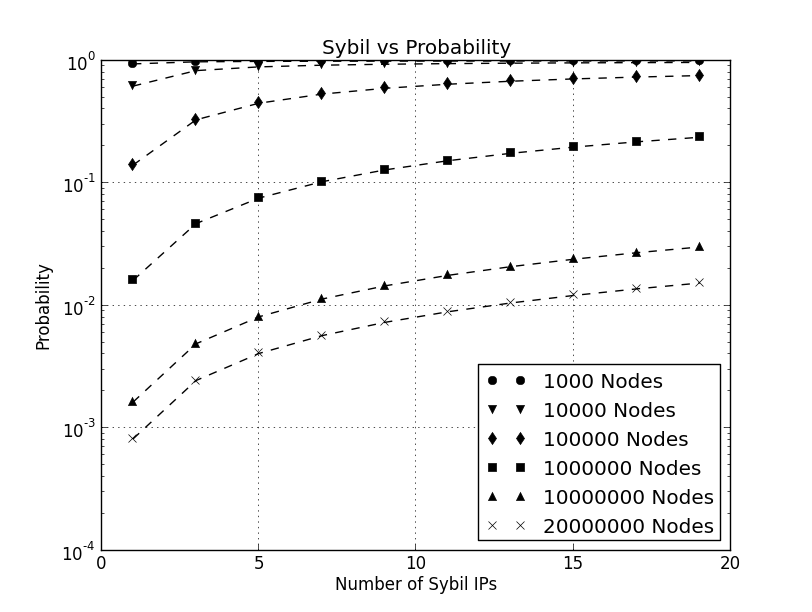
\includegraphics[width=1\linewidth]{figs/ip_prob_all}
	\caption[foo]{Our simulation results.  
		The $x$-axis corresponds to the number of IP addresses the adversary can bring to bear.
		The $y$-axis is the probability that any chosen region has been mashed.
		Each line maps to a different network size of $n$.
		The dashed line corresponds to values from Equation \ref{eq:bad}: $ P_{bad\_neighbor} =  \frac{num\_ips \cdot 16383}{num\_ips \cdot 16383 + n - 1}$}
	\label{fig:exp2}
\end{figure}


\begin{figure}
	\centering
	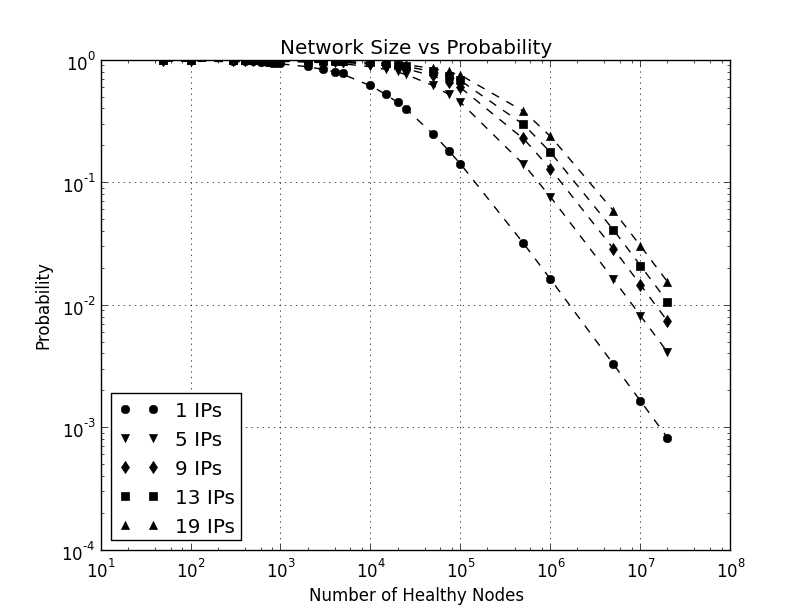
\includegraphics[width=\linewidth]{figs/size_prob_all}
	\caption[a]{These are the same as results shown in Figure \ref{fig:exp2}, but our $x$-axis is the network size $n$ in this case.  
		Here, each line corresponds to a different number of unique IP addresses the adversary has at their disposal.}
	\label{fig:size_prob_all}
\end{figure}



\begin{table}\small
	\centering
	\caption{Selection of results for Nearest Neighbor Eclipse.}  %The Fraction of regions injected is the percentage of all regions for which the adversary could inject a Sybil with the suitable key. The Sybil/Region measure is how many Sybils were available to inject a particular region on average.}
	\label{tab:exp2}
	\begin{tabular}{|r|r|r|r|}
		\hline
		IPs & Network Size &  Success Rate & Sybils/Region \\ \hline
		1 & 5000 & 0.7748 & 3.2762 \\ \hline
		1 & 5000000 & 0.0032654 & 0.0032768 \\ \hline
		1& 10000000 & 0.0016364 & 0.0016384 \\ \hline
		1 & 20000000 & 0.00081865 & 0.0008192 \\ \hline
		5 & 5000 & 0.9444 & 16.381 \\ \hline
		5 & 5000000 & 0.0161208 & 0.016384 \\ \hline
		5 & 10000000 & 0.0081223 & 0.008192 \\ \hline
		5 & 20000000 & 0.0040801 & 0.004096 \\ \hline
		11 & 5000 & 0.9708 & 36.0428 \\ \hline
		11 & 5000000 & 0.0347646 & 0.0360448 \\ \hline
		11 & 10000000 & 0.0177117 & 0.0180224 \\ \hline
		11 & 20000000 & 0.008932 & 0.0090112 \\ \hline
		19 & 5000 & 0.9834 & 62.2452 \\ \hline
		19 & 5000000 & 0.058562 & 0.0622592 \\ \hline
		19 & 10000000 & 0.0301911 & 0.0311296 \\ \hline
		19 & 20000000 & 0.01532465 & 0.0155648 \\ \hline
	\end{tabular}
	
	
\end{table}

%NEED TO TEST TO SEE WHAT NEEDED TO ATTACK 50,000,000 size network, twice the size of the BitTorrent network.  CAN WE?
%Each experiment took less than a second to perform.
Our results show that an adversary, given only modest resources, can inject a Sybil in between the vast majority of successive nodes in moderately sized networks.
In a large network, modest resources still can be used to compromise more that a third of the network, an  important goal if the adversary  wishes to launch a Byzantine attack.

Our results match values predicted by Equation \ref{eq:bad}.
However, this experiment only covers the short links of the network, but not the long distance links.

% PLOT for LD50 values for IPS vs Network Size



\subsection{Experiment 3: Complete Eclipse via Sybil on Chord}
\label{sec:chord}
We extended the previous experiment by considering the long-distance hops of each node in addition to the short-range links of the DHT.
We choose to model an attack on a P2P system built using Chord \cite{chord}.


We chose to model Chord for a number of reasons.
Chord is an extremely well understood DHT and is very simple to evaluate using simulations.
Nodes in Chord generates long distance links independent of information provided by other nodes, rather than directly querying neighbors.
This minimizes the opportunities adversaries have to poison the node's routing table via false advertisements, which can be on other DHTs such as Pastry \cite{pastry}. 
This makes the Sybil attack the most straightforward means of effecting an Eclipse attack on a Chord network.

Nodes in Chord have $m$ long-range links, one for each of the bits in the keys, which is 160 in our experiments.
Each of node $a$'s long-range links points to the node with the lowest key $\geq a + 2^{i} \mod 2^{m}, 0 \leq i \leq 160$.

However, many of the fingers are redundant and point to the nearest neighbor.
As we have mentioned, on average, nodes are $\frac{2^{m}}{n}$ distance apart.
The smaller the network, the further apart nodes are, and therefore each  node has more redundant fingers and is easier to attack.

The attack is very similar to the Nearest Neighbor attack demonstrated above.
Beside injecting a node in between successive nodes, the attacker also attempts to place a Sybil in between each of the long-range links.
We simulated this attack under the same parameters as above and are presented in Table \ref{tab:exp3}.


\begin{figure}
	\centering
	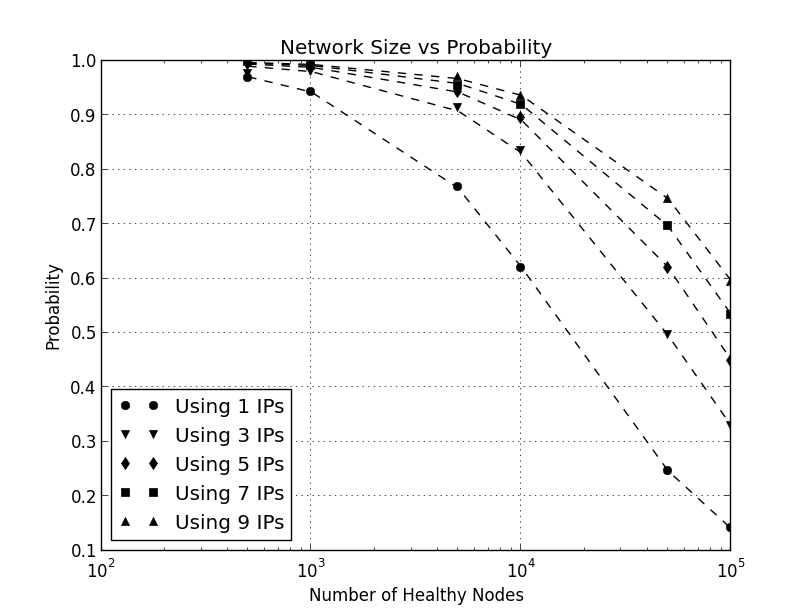
\includegraphics[width=\linewidth]{figs/size_occlusion_chord}
	\caption{This graph shows the relationship between the network size and the probability a particular link in Chord, adjacent or not, can be mashed.
		The dotted line traces the line corresponding to the Equation \ref{eq:bad}: $ P_{bad\_neighbor} =  \frac{num\_ips \cdot 16383}{num\_ips \cdot 16383 + n - 1}$}
	
	\label{fig:exp3}
\end{figure}



\begin{table}\small
	
	\caption{Selection of results for a Sybil attack on Chord.} % The percentage of links occluded is the percentage of long range links from healthy nodes that connect to Sybil nodes. 
	%The Occlusion per node measures how many of the 160 long range links lead to a Sybil on average.  
	%We ignore the predecessor links since it is not used for routing.}
	\label{tab:exp3}
	
	\begin{tabular}{|r|r|r|r|}
		\hline 
		IPs & Network Size &   Success Rate & Occlusions/Node \\ \hline
		1 & 1000 & 0.94186875 & 150.699 \\ \hline
		1 & 10000 & 0.618480625 & 98.9569 \\ \hline
		1 & 100000 & 0.141753625 & 22.68058 \\ \hline
		3 & 1000 & 0.97915625 & 156.665 \\ \hline
		3 & 10000 & 0.83425 & 133.48 \\ \hline
		3 & 100000 & 0.3286290625 & 52.58065 \\ \hline
		5 & 1000 & 0.988725 & 158.196 \\ \hline
		5 & 10000 & 0.894415 & 143.1064 \\ \hline
		5 & 100000 & 0.4488916875 & 71.82267 \\ \hline
		7 & 1000 & 0.99091875 & 158.547 \\ \hline
		7 & 10000 & 0.919071875 & 147.0515 \\ \hline
		7 & 100000 & 0.5337635625 & 85.40217 \\ \hline
		9 & 1000 & 0.9948125 & 159.17 \\ \hline
		9 & 10000 & 0.935495625 & 149.6793 \\ \hline
		9 & 100000 & 0.5936118125 & 94.97789 \\ \hline
		
		
	\end{tabular}
	
	
	
\end{table}





Surprisingly, the percentage of links from healthy nodes that connect to Sybil nodes follows Equation \ref{eq:bad} and the results from \ref{sec:exp2}.
This means performing a Nearest Neighbor Eclipse provides the same results as actively blocking all the long range links in the network.

Our results show that an attacker needs only to focus their efforts on compromising the links between adjacent nodes to attack all the links in the network.


We can calculate that the number of IP addresses needed to compromise half the links in a 20,000,000 node network is 1221 IP addresses.
While this seems like a daunting number of IP addresses, cloud computing has made solutions for an attacker much more accessible and affordable to attackers.
At the time of writing, it would cost \$43.26 USD to use 1221 instances for an hour on Amazon's Elastic Cloud Compute service.
In fact, one of the attacker launching a Sybil attack was identified as having an IP address associated with Amazon's Elastic Cloud Compute \cite{sybilbit}.


%\subsubsection{Plaxton Based networks}


%\section{Masking the Attack}
%Now that we have established that a Sybil attack can be performed with great ease, our focus now turns to avoiding detection.
%The only surefire way to achieve this is by preventing a node from seeing 
%We need a different IP for each point surrounding our victim.  In the Nearest-Neighbor attack, we need a 

%We can reduce this into an interesting graph coloring problem.


%The hard maximum, in general, is $m$ separate IP addresses, one for each bit in a $\log n$ routing/routing table DHT.
%Recall that the vast

\section{Conclusions and Future Work}\label{sec:conclusions-and-future-work}
%\section{Simple Load Balancing Injection Framework}
\label{sec:horror}

Our analysis and experiments show that an adversary with limited resources can easily compromise a P2P system and occlude the majority of the paths between nodes.
All that is required is a small number of IP addresses and the unassigned ports.
This implies system privileges are not required.
A successful attack effectively prevents nodes from talking to one another without sending messages through Sybils.
The Sybils can eavesdrop on the messages, actively reroute them, or substitute malicious data.
Mashing can also be used prevent malicious behavior.
Sybils inserted in a P2P botnet by this approach could effectively interfere with command and control functions to shut down the botnet \cite{white2010overcoming}.
Future research would involve developing an appropriate mashing algorithm for a given botnet.


Our discussion has primarily concerned Chord.
We did not simulate an attack on Mainline DHT  \cite{mainline}, the Kademlia \cite{kademlia} based DHT used as the backend of BitTorrent, because it is completely unnecessary to perform any mashing.
In MLDHT, a node ID is not chosen by hashing an IP and port combination, but by picking an address uniformly at random between 0 and $2^{160}-1$.
Since the choice of node ID in MLDHT is left to the client, there is no impediment to a Sybil attack. 
Research has examined MLDHT's vulnerability to Sybil attacks \cite{sybilbit} and detected entities performing the attack on MLDHT.

A hash function over a unique identifier might seem to provide a level of protection against a Sybil attack.
Our research demonstrates that using a SHA1 hash of the IP address and port number is no defense against a Sybil attack. 
We show that the adversary can easily mash Sybil into desirable locations.
%A big difference is their honeypots target those who respond to everything.


However, the mashing process can be used in non-malicious purposes to benefit a DHT.
The SHA1 hash has an evenly distributed output. 
Most sets of meaningful keys will not have a uniform distribution \cite{shannon2001mathematical}
Some nodes will be responsible for larger regions than others and therefore will be responsible for a larger portion of the data.
If a node can detect when a peer is overloaded, the node can inject a virtual node into the region to shoulder some of the load.
The load could be defined by the size of the region or by the volume of traffic.

A network implementing this load-balancing strategy would be self-adaptive.
Nodes in this type of self-adaptive network would have a limited number of virtual nodes to mash.
This limit would protect nodes from becoming overloaded themselves and ensure network stability.
We discuss how we can implement this in Chapter \ref{chapter:auto-balance}. % done
	\chapter{Autonomous Load Balancing in a Distributed Hash Table}
\label{chapter:auto-balance}




%http://michiel.buddingh.eu/distribution-of-hash-values

\section{Introduction}

%\subsection{2-4 sentences telling people what you will talk about in the paper}

%\subsection{What are DHTs}
Distributed Hash Tables (DHTs) are a class of well researched decentralized key-value storage systems.
DHTs are most frequently used to construct the overlays of P2P file-sharing systems, such as the incredibly popular BitTorrent \cite{bittorrent}.
DHTs have also been used in many unorthodox applications, such as machine learning \cite{liparameter} and, most relevant for our discussion, distributed computing \cite{chordreduce}.

Our previous research \cite{chordreduce} examined using a DHT as the organizing mechanism for a distributed platform.
This enabled us to create an exceptionally fault tolerant distributed computing platform that was easy to setup and could be run in a completely decentralized P2P environment.

% Copy into disseration start here
%\subsection{What is the significance of the hash function }
One of key components of a Distributed Hash Table is a cryptographic hash function, most commonly SHA1 \cite{sha1}.
Distributed Hash Tables rely on this cryptographic hash function to generate identifiers for data stored on the network.
The cryptographic hash of the filename or other identifier for the data is used as the location of the file or data in the network.
It can also be used to generate the identifiers for nodes in the network.

Ideally, inputing random numbers into a cryptographic hash function should produce a uniformly distributed output.
However, this is impossible in practice \cite{hash-outputs} \cite{thomsen2005cryptographic}.

In practice, that means given any DHT with files and nodes, there will be an inherent imbalance in the network.
Some nodes will end up with a lion's share of the keys, while other will have few responsibilities (Table \ref{tab:medianLoads}).


This makes it especially disheartening to try and ensure as even a load as possible.
We cannot rely on a centralized strategy to fix this imbalance, since that would violate the principles and objects behind creating a fully decentralized and distributed system.

Therefore, if we want to create strategies to act against the inequity of the load distribution, we need a strategy that individual nodes can act upon autonomously.
These strategies need to make decisions that a node can make at a local level, using only information about their own load and the topology they can see.


\subsection{Motivation}
The primary motivation for us is creating a new viable type of platform for distributed computing.
Most distributed computing paradigms, such as Hadoop \cite{hadoop}, assume that the computations occur in a centralized environments.
One enormous benefit is a centralized system has much greater control in ensuring load-balancing.

However, in an increasingly global world where computation is king and the Internet is increasingly an integral part of everyday life, single points of failure failures quickly become more and more risky.
Users expect their apps to work regardless of any power outage affecting an entire region.
Customers expect their services to still be provided regardless of any.
The next big quake affecting the the San Andreas fault line is a matter of when, not if.
Thus, centralized systems with single points of failure become a riskier option and decentralized, distributed systems the safer choice.


Our previous work in ChordReduce \cite{chordreduce} focused on creating a decentralized distributed computing framework based off of the Chord Distributed Hash Table (DHT) and MapReduce.
ChordReduce can be thought of a more generalized implementation of the concepts of MapReduce.
One of the advantages of ChordReduce can be used in either a traditional datacenter or P2P environment.\footnote{The other one being that new nodes could join during runtime and receive work from nodes doing computations.}
Chord (and all DHTs) have the qualities we desire for distributed computing: scalability, fault tolerance, and load-balancing.

Fault tolerance is of particular importance to DHTs, since their primary use case is P2P file-sharing, such as BitTorrent \cite{bittorrent}.
These systems experience high levels of churn-- disruptions to the network topology as a result of nodes entering and leaving the network.
ChordReduce had to have the same level of robustness against churn that Chord did, if not better.

During our experiments with ChordReduce, we found that high levels of churn actually made our computations run \textit{faster}.
We hypothesized that the churn was effectively load-balancing the network.

\subsection{Objectives}
This paper serves to prove our hypothesis that churn can load balance a Distributed Hash Table.
We also set out to show that we can use this in a highly controlled manner to greater effect.

We present three additional strategies that nodes can use to redistribute the workload in the network.
Each of these three strategies relies on nodes creating virtual nodes, and so that they are represented multiple times in the network.
The idea behind this is that a node with low work can create virtual nodes to seek out and acquire work from other nodes.

This tactic is the same one used in the Sybil \cite{sybil} attack, but limited in scope and performed for altruistic and beneficent reasons, rather than malicious ones.
Consequently, we'll call our virtual nodes in this scenario Sybils for clarity and brevity.
None of the strategies require a centralized organizer, merely a way for a node to check the amount of files or tasks it and its Sybils are responsible for.


We also want to show how distributed computing can be performed in a heterogeneous environment.
We want to see if our strategies result in similar speedups in both homogeneous and heterogeneous environments.
%\subsection{Summary}

%\section{Previous Work}
%
%
%ChordReduce \cite{chordreduce} is designed as a more abstract framework for MapReduce, able to run on any arbitrary distributed configuration.
%ChordReduce leverages the features of distributed hash tables to handle distributed file storage, fault tolerance, and lookup.
%We designed ChordReduce to ensure that no single node is a point of failure and that there is no need for any node to coordinate the efforts of other nodes during processing.

\section{How Work Is Distributed in DHTs: A Visual Guide}
%In this section, we display graphs to give a visual representation of how work is distributed in a Chord \cite{chord} network

As we have previously mentioned, many DHTs use a cryptographic hash function to choose keys for nodes and data.
However, no cryptographic hash function can uniformly distribute it's outputs across its range. 

\begin{table}
	\centering
	\caption{The median distribution of tasks (or files) among nodes.  We can see the standard deviation is fairly close to the expected mean workload ($\frac{tasks}{nodes}$). Each row is the average of 100 trials.}
	\begin{tabular}{r r r r}
		Nodes & Tasks & Median Workload & $\sigma$ \\ \hline
		1000 & 100000 & 69.410   &  137.27  \\
		1000 & 500000 & 346.570  &  499.169 \\
		1000 &1000000 & 692.300  &  996.982 \\
		
		5000 & 100000  & 13.810 & 20.477 \\ 
		5000 & 500000  & 69.280 & 100.344 \\ 
		5000 & 1000000 &138.360 & 200.564 \\ 
		
		10000 & 100000 & 7.000   &  10.492 \\
		10000 & 500000 & 34.550  &   50.366 \\
		10000 & 1000000& 69.180  &  100.319 \\
	\end{tabular}
	\label{tab:medianLoads}
\end{table}




\begin{figure}
	\centering
	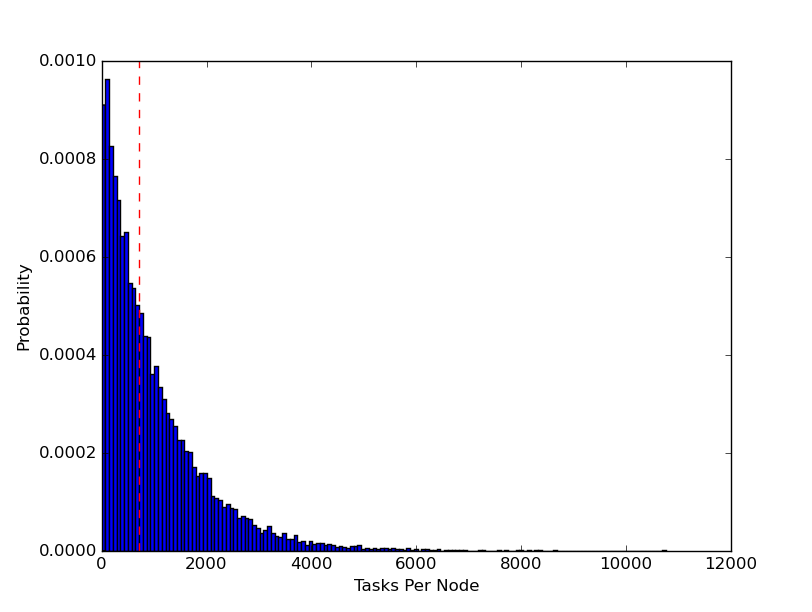
\includegraphics[width=0.7\linewidth]{figs/workloadDistribution}
	\caption[foo]{The probability distribution of workload in a DHT with 1000 nodes and 1,000,000 tasks or files.  The vertical dashed line designates the median.  Keys were generated by feeding random numbers into the SHA1 hash function \cite{sha1}, a favorite for many distributed hash tables.}
	\label{fig:workloadDistribution}
\end{figure}

An example Chord DHT.
Each node and task is given a 160-bit identifier \texttt{id} that is mapped to location $ (x,y) $ on the perimeter of the unit circle via the equations $ x = \sin\left( \frac{ 2 \pi \cdot id}{2^{160}} \right)$ and $ y = \cos\left( \frac{ 2 \pi \cdot id}{2^{160}} \right)$. 
Note that some of the nodes cluster right next to each other, while other nodes have a relatively long distance between each other along the perimeter.  
The most blatant example of this is the node located at approximately $(-0.67, 0.75)$, which would be responsible for all the tasks between that and the next node located counterclockwise.
That node and the node located at about $(-0.1, -1)$ are responsible for approximately half the tasks in the network.

\begin{figure}
\centering
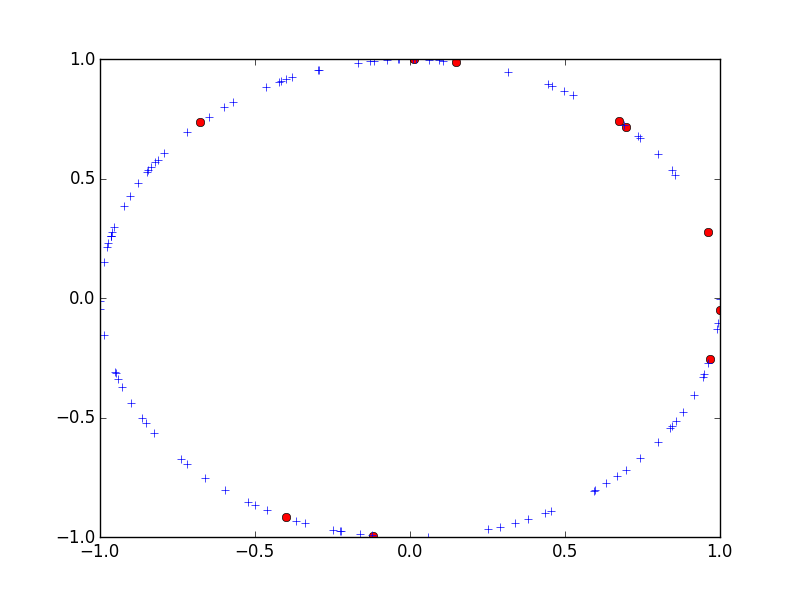
\includegraphics[width=0.7\linewidth]{figs/exampleChordDistribution}
\caption[Distribution of Nodes and Tasks in a Chiord DHT]{A visual example of data and nodes in a Chord DHT with 10 nodes (represented by red circles) and 100 tasks (blue pluses). Nodes are responsible for all the tasks that fall along the perimeter between themselves and their predecessor, which is the closest node counterclockwise.}
\label{fig:exampleChordDistribution}
\end{figure}



\section{Simulation}
\label{sec:auto-simulation}

%We simulate an UrDHT Voronoi based-network in multiple dimensions. \footnote{UrDHT in one dimension is a Chord ring with the definition of responsibility changed to a node being responsible to all data closest to it. A 2-dimensional network will emulate the performance of CAN.}


We will be simulating our strategies on a Chord distributed hash table \cite{chord}, although it is fairly straightforward to implement our strategies for other, more complex DHTs.
Nodes in a Chord ring are given an ID, drawn from a cryptographic hash function, typically SHA1 \cite{sha1}.
Any data in the network is given a key in a similar manner.
Nodes are responsible for all the keys between their predecessor's ID and their own.

We assume that the network starts our experiments stable and the data necessary already present on the nodes and backed-up.
The following analysis and simulation relies on an important assumption about DHT behavior often assumed but not necessarily implemented.


We assume that nodes are active and aggressive in creating and monitoring the backups and the data they are responsible for.
%Specifically, we will assume it takes  $T_{detect}$ time for a node to detect a change in their responsibility or to detect a new node to hand a backup to and that this check is performed regularly. 
We have demonstrated the effectiveness and viability of implementing an active backup strategy in other work \cite{chordreduce} \cite{urdht}.
As previously mentioned, we also assume nodes have the ability to examine the amount of work they have and know how many tasks or pieces of data exist for a particular job.

Another assumption is that nodes do not have control in choosing their IDs from the range of hash values.
This means that nodes cannot automatically change their spacing to ensure they are all evenly spread out across the network.
Likewise, nodes cannot create necessarily create Sybils exactly where they would like, but would have to search for an appropriate ID in between two other nodes.
We discussed this process in previous work and showed that it is extremely quick for a node to do so \cite{sybil-analysis}.



%Smaller chunking results in more files spread throughout the network and a greater chance of the data being evenly spread across the network 


%The chances of a critical failure happening within a time interval $ T $ is the chances of some chain or cluster of nodes responsible for a single record dying within $ T $:
%
%$$r^{s}$$
%
%Where $ r $ is the failure rate over that time interval and $s$ is the number nodes storing that record, either as a primary system, or a backup.
%Incidentally, this time interval $T = T_{detect} + T_{transfer} $
%


\subsection{The Parameters}

Our simulations relied on a great number of parameters and variables.
We present each of them below.

\subsubsection{Constants and Terminology}

First, we'll define informally define the vocabulary we use to discuss our simulations.

\begin{description}
	\item [Tick] In a simulation, normal measurements of time such as a second are completely arbitrary.  
	We will be using an abstract \textit{tick} to measure time.  
	We consider the tick the amount of time it takes a node to complete one task (or more depending on our variables, see below) and perform the appropriate maintenance to keep the network consistent and healthy.\footnote{If we need to be more concrete, define a tick as a New York Second, which is ``the period of time between the traffic lights turning green and the cab behind you honking.''\\-- Terry Pratchett}
	\item [Maintenance] We assume nodes use the active, aggressive strategy from ChordReduce and UrDHT \cite{chordreduce} \cite{urdht}.
	Every maintenance cycle, each node checks and updates its list of neighbors (successors and predecessors in Chord) and responds appropriately. 
	We assume that a tick is enough time to accomplish at least one maintenance cycle.
	\item[Task] We measure the size of a distributed computing job in tasks.
	Each task has a key that corresponds to the key of a file or chunk of a file stored on the network.
	We assume that it takes a tick for a node to consume at least one task.
	\item [IDs and Keys] 
	We will be using SHA-1 \cite{sha1}, a 160-bit hash function, to generate node IDs and keys for tasks.  
	We assume each task's key corresponds to some piece of data with the same key, a scheme we used in  our previous work on ChordReduce \cite{chordreduce}.
\end{description}

\subsubsection{Experimental Variables}
We tested a number of strategies and variables that could affect each strategy.
While we believed the overall strategy would result in largest differences in runtime, we wanted to see what effects, if any, each of the variables would have on a particular strategy.

\begin{description}
	\item [Strategy] We use several different strategies, each discussed in Section \ref{sec:strategies}: churn, random injection, neighbor injection, and invitation.
	Each of these strategies differs in how nodes attempt  to autonomous balance the workload of the network.
	None of the strategies require centralized organization.
	\item [Homogeneity]  This variable controls whether the network is homogeneous or not.
	In a homogeneous network, each node has the same strength, which dictates how much work is consumed per a tick and how many Sybils it can create.
	In a heterogeneous network, each node has a strength chosen uniformly at random from 1 to \texttt{maxSybils}.
	\item [Work Measurement] This variable dictates how much work is consumed in a tick.
	Each node can either consume a single task per a tick or their strength's worth of tasks per a tick.
	\item [Network Size]  How many nodes start in the network.  
	We assume that this can grow during the experiment, either via churn or by creating Sybils.
	We discuss how this works in Sections \ref{sec:strat-churn} and \ref{sec:strat-randomInject}.
	\item [Number of Tasks] We measure the size of of a job in tasks.
	This number is typically a few orders of magnitude greater than the network size.
	\item [Churn Rate] The churn rate is a float between 0 and 1.
	This represents both the chance each individual node has of leaving (or joining) the network each tick.
	It also corresponded to the fraction of nodes we expect to leave the network each tick.
	Churn can be self induced or a result of actual turbulence in the network.
	Like most analyses of churn \cite{marozzo2012p2p}, we assume churn is constant throughout the experiment and that the joining and leaving rate are equal.
	\item [Max Sybils] \texttt{maxSybils} is the maximum number of Sybils a node can have at once.
	\item [Sybil Threshold] The \texttt{sybilThreshold} dictates the number of tasks a node must have before it can create a Sybil.
	\item [Successors] The number of successors each node keeps track of.  
	Nodes also keep track of the same number of predecessors.
	
\end{description}

We also considered using a variable noted as the \texttt{AdaptationRate}, which was the interval at which nodes decided whether or not to create a Sybil.
Preliminary experiments showed \texttt{AdaptationRate} to have a minimal effect on the runtime, so it was removed.

\subsubsection{Outputs}
The most important output was the number of ticks it took for the experiment to complete.
We compared this runtime to the what we call the ``ideal runtime,'' which is our expected runtime if the every node in the network was given an equal number of tasks and performed them without any churn or creating any Sybils.
For example, consider a network with 1,000 nodes and 100,000 tasks, where each node consumes a single task each tick. 
This network has an ideal runtime of 100 ticks ($ \frac{100000}{1000} = 100$).\footnote{The ideal runtime also happens to be the average number of tasks per node. An interesting, but mathematically unsurprising, coincidence with a few consequences for our data collection.} 

We used these to calculate a ``runtime factor,'' the ratio of the experimental runtime compared to the ideal runtime.
For example, in the network from our previous example took 852 ticks to finish, its factor is 8.52.
We prefer to use this runtime factor for comparisons since it allows us to compare networks of different compositions, task assignments, and other variables.

We also collected data on the average work per tick and statistical information about how the tasks are distributed throughout the network.
We additionally performed detailed observations of how the workload is  distributed and redistributed throughout the network during the first 50 ticks.

\section{Strategies}
\label{sec:strategies}

For our analysis, we examined four different strategies for nodes to perform autonomous load balancing.
We first show the effects of churn on the speed of a distributed computation.
We then look a three different strategies for in which nodes take a more tactical approach for creating churn and affecting the runtime.

Specifically, nodes perform a limited and controlled Sybil attack \cite{sybil} on their own network in an effort to acquire work with their virtual nodes.
Our strategies dictate when and where these Sybil nodes are created.

We discuss the effectiveness of each of the strategies and present the results of our simulations in Section \ref{sec:autonomous-results}.



\subsection{Induced Churn}
\label{sec:strat-churn}
Our first strategy, \textit{Induced Churn}, relies solely on churn to perform load balancing.
This churn can either be a product of normal network activity or self-induced.\footnote{All distributed systems experience churn, even if only as hardware failures.}
By self-induced churn, we mean that each node generates a random floating point number between 0 and 1.
If the number is $\leq churnRate$, the node shuts down and leaves the network and gets added to the pool of nodes waiting to join.

Similarly, we have a pool of waiting nodes that begins the same initial size as the network.
When they generate an appropriate random number, they join the network and leave the waiting pool.
We assume that nodes enter and leave the network at the same rate.
Because the initial size of the network and the pool of waiting nodes is the same and nodes move between one another at the same random rate, the size of either does not fluctuate wildly.

As we have previously discussed, nodes in our network model actively back up their data and tasks to the a number of successors in case of failure.
In addition, when a node joins, it acquires all the work it is responsible for.
While this model is rarely implemented for DHTs, it is discussed \cite{kademlia} and often assumed to be the way DHTs operate. 
We have implemented it in ChordReduce\cite{chordreduce} and UrDHT\cite{urdht} and demonstrated that the network is capable from recovering from quite catastrophic failures and handling ludicrous amounts of churn.

The consequences of this are that a node suddenly dying is of minimal impact to the network.
This is because a node's successor will quickly detect the loss of the node and know to be responsible for the node's work.
Conversely, a node joining in this model can be a potential boon to the network by joining a portion of the network with a lot of tasks and immediately acquiring work.

This strategy acts as a baseline with which to compare the other strategies, as it is no more than a overcomplicated way of turning machines off and on again. 
All strategies below are attempts to do better than random chance.
However, this strategy also serves to confirm the speedup phenomenon we observed in our previous work on a distributed, decentralized MapReduce framework \cite{chordreduce}.

\subsection{Random Injection}
\label{sec:strat-randomInject}
Our second strategy we dubbed \textit{Random Injection}.
In this strategy, once a node's workload was at or below the \texttt{sybilThreshold}, the node would attempt to acquire more work by creating a Sybil node at a random address.

A node compares its workload to the \texttt{sybilThreshold} and decides whether or not to make a Sybil.
This check occurs every 5 ticks.
A node cam also have multiple Sybils, up to \texttt{maxSybils} in a homogeneous network or the node's \texttt{strength} in a heterogeneous network.\footnote{No benefit was shown by increasing \texttt{maxSybils} beyond 10.}
If a node has at least one Sybil, but no work, it has its Sybils quit the network.
We limit each node to creating a single Sybil during this decision to avoid overwhelming the network.

%As we discuss in Section \ref{sec:autonomous-results}, this strategy is surprisingly effective and comes close to ideal runtimes.



\subsection{Neighbor Injection}
\label{sec:strat-neighbor}
\textit{Neighbor Injection} also creates Sybils, but in this case, nodes act on a more restricted range in an attempt to limit the network traffic.
Nodes with \texttt{sybilThreshold} or less tasks attempt to acquire more work by placing a Sybil among it's successors.
Specifically, it looks for the biggest range among it's successors and creates a Sybil in that range.

This range strategy of finding the largest range and injecting assumes that the node with the largest range of responsibility will have been allocated the most work.
This is a sensible assumption since the larger the range of a node's responsibility, the more \textit{potential} tasks it can receive. 
We compare this estimation strategy to actually querying the neighbor and asking how many tasks they have.
An estimation, if accurate, would be preferable to querying the nodes as an estimation can be done without any communication with the successor nodes.

To avoid constant spamming of a range, once a node creates a Sybil, but does not acquire work, it may be advisable to mark that range as invalid for Sybil nodes so nodes don't keep trying the same range repeatedly. 


\subsection{Invitation}
The \textit{Invitation} strategy is the reverse of the Sybil injection strategies.
In  this strategy, nodes with a higher than desired level of work announces it needs help to its predecessors.
The predecessor with least amount of tasks less than or equal to the \texttt{sybilThreshold} creates a Sybil to acquire work from the node.
It is possible for an invitation to get more work to be refused by anyone if no  predecessor is at the \texttt{sybilThreshold} or each predecessor has too many Sybils.
Nodes determine whether or not they are overburdened using the \texttt{sybilThreshold}.



\section{Results Of Experiments}
\label{sec:autonomous-results}

We now briefly summarize the results of our simulation before discussing each more in depth below.
First, we confirmed that churn, even at low levels, can speed up the execution of a distributed computation by dynamically load balancing the network.
However, our best strategy was random injection, which managed to have a runtime factor which approached close to 1.

All the raw data can be found online \cite{simulation-data}.
Files are sorted by the strategy used, the network size,  and number of tasks and include the both the results of each individual run and the averages of each 100 trials for a particular set of variables.
Each trial is linked with a seed for the pseudorandom number generator and can be fully reproduced.


\subsection{Churn}


Our results confirmed our hypothesis from ChordReduce \cite{chordreduce}.
Churn has a profound and significant impact on the network's computation, and this effect is more pronounced with higher rates of churn.
We show this in Figure \ref{fig:churnVsTime}, which plots the runtime of the distributed computation against the level of churn in the network.
This particular network contained 1000 nodes and 100000 tasks.


\begin{figure}
	\centering
	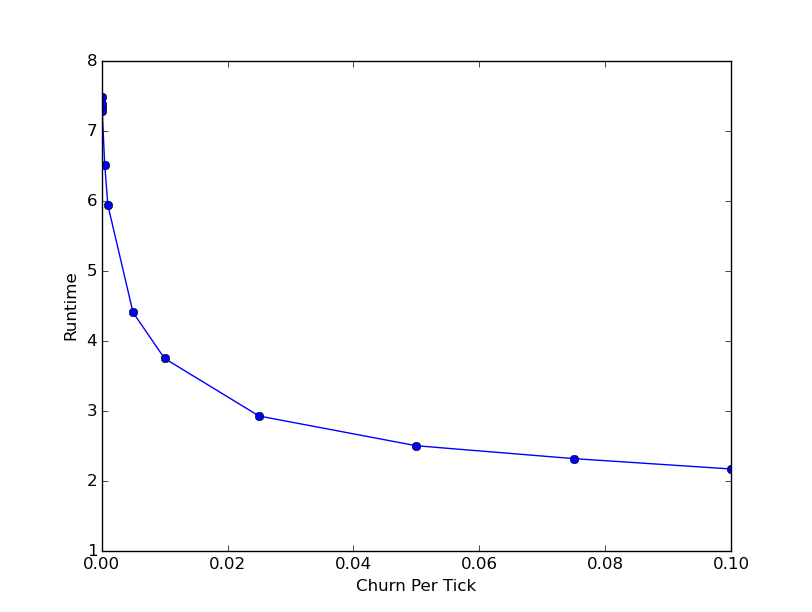
\includegraphics[width=0.7\linewidth]{figs/churnVsTime}
	\caption[Churn vs Runtime factor]{This graph shows the effect churn has on runtime in a distributed computation.
		Runtime is measured as how many times slower the computation runs than an ideal computation, where each node receives an equal number of tasks.
		The lower the runtime factor, the closer it is to an ideal of 1.
		Neither the homogeneity of the network nor work measurement had a significant effect on the runtime.}
	\label{fig:churnVsTime}
\end{figure}


We note the significantly diminishing returns that occur after a churn rate of 0.01.
One facet not captured by our simulations, but is significant, is the rising maintenance costs after that point.
The makes any amount of churn after a certain point prohibitively expensive.

Also graph average work per tick (Figure \ref{fig:churnVsWork})
\begin{figure}
\centering
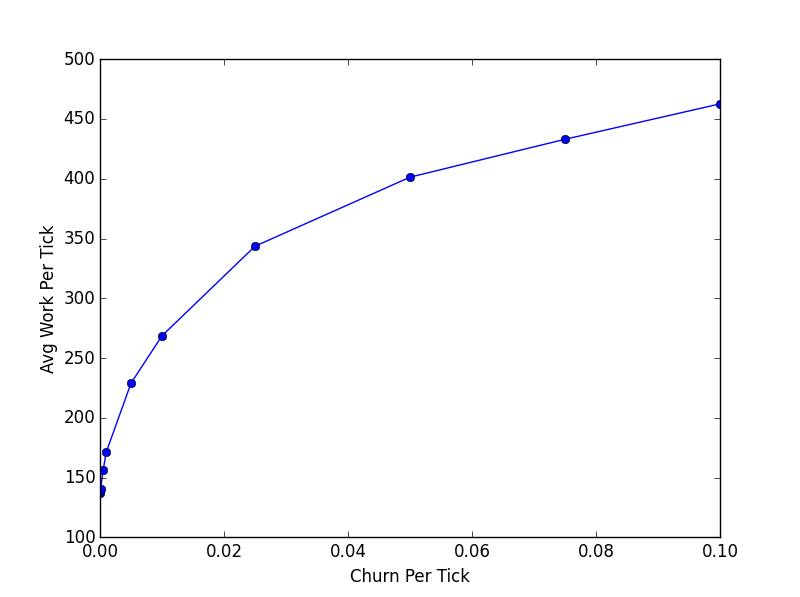
\includegraphics[width=0.7\linewidth]{figs/churnVsWork}
\caption[Churn vs average work per tick]{We can see that this is a mirror image of Figure \ref{fig:churnVsTime}.}
\label{fig:churnVsWork}
\end{figure}


How did scaling affect the network?  
Network runtime is affected by scaling.


\subsection{Random Injection}

The strategy of having under-utilized nodes randomly create Sybil nodes works phenomenally well, approaching very close to the ideal time.
%specifics


Ratios seem to have similar runtimes, but smaller networks run slightly faster.
smaller network faster
0.086 1h100k 1k1m 
0.28 1h10k 


However, the larger ratio networks handled heterogeniety much better, with the worst heterogenous run time being 1.955, compared to 4.052 on  the smaller ratio networks


Sybil Threshold had an effect in homogeneous networks but no effect in heterogeneous networks.
In our 1k100k and 1h1k experiment, a homogenous network where each node completed one task per a tick, this amounted to an reduction of at least 0.1 runtime factor.
The effect was more pronounced when networks could complete a number of tasks equal to their strength each tick, reducing the runtime factor by at least 0.2.


However, we saw no corresponding speedup in the 1k1m and 1h100k networks.
We also found the \texttt{sybilThreshold} had no discernible effect on the runtime of heterogeneous networks.
This suggests the effect of a particular \texttt{sybilThreshold} is tied to the ratio of nodes to tasks and that the larger the ratio, the less room there is to improve.


Churn had no positive impact on the runtime factor and at higher levels could begin having an extremely minor impact when churn is at 0.01 per tick, increasing the average runtime factor by approximately 0.06 
\subsection{Neighbor Injection}


On average, the strategy of probing each of the neighbors before inserting, rather than estimating 
\subsection{Invitation}

In invitation, churn losses can be greatly detrimental.

\section{Future Work}

As mentioned in Section \ref{sec:auto-simulation}, we made the assumption that nodes cannot choose their own ID and must rely on the strategies described in Chapter \ref{chapter:sybil}  \cite{sybil-analysis} for creating a Sybil with the appropriate ID.
However, if this assumption was removed, this presents even more strategies for nodes to autonomously load-balance. % done 
	\chapter{Conclusion}
\label{chapter:conclusion}
Distributed Hash Tables (DHTs) are extremely powerful frameworks for distributed applications that are based off the simple and powerful hash tables.
Because DHTs were designed with P2P applications in mind, DHTs are scalable, fault-tolerant, and load-balancing.
These are exactly the qualities needed in a distributed computing framework.

We created a new DHT called VHash, which was based off the relationship we discovered between the DHTs and Voronoi tessellation.
VHash is a DHT that operates over a multidimensional space, which allows the embedding of arbitrary metrics into this space.
We showed that we can optimize latency in VHash to obtain faster lookup speeds than a traditional DHT, such as Chord.
The key to VHash is our Distributed Greedy Voronoi Heuristic (DGVH).
DGVH is a sufficiently accurate and fast approximation of Delaunay triangulations.
Aside from its application in VHash, DGVH's applications extend to other areas, such as wireless sensor networks.

We have also shown in the previous chapters that we were able to create a prototype distributed computing application \cite{chordreduce} based on the Chord DHT \cite{chord}.
ChordReduce, as we named it, demonstrated how MapReduce could be performed on the Chord distributed hash table.
As a DHT, ChordReduce is completely decentralized and fault-tolerant, able to handle  nodes entering and leaving the network during churn.
We demonstrated that ChordReduce can efficiently distribute a problem whilst undergoing significant churn and achieve a significant speedup.

During our experiments with ChordReduce, we found an anomaly in which a computation undergoing a significantly high level of churn finished twice as fast than when no churn was involved.
This implied to us that there the churn was effectively shuffling around the nodes such that nodes with no work were taking work from nodes with large amounts of work.
We want to use this implication  develop a more intelligent autonomous load-balancing mechanism.
Such a mechanism would allow underworked nodes to steal work from overworked nodes in the network.

Part of autonomous load-balancing will involve exploiting heterogeneity in the network.
We can do this by having more powerful nodes take a proportionally higher amount of work.
This involves a process we dubbed \textit{mashing}, which we originally used to analyze the Sybil attack on DHTs \cite{sybil-analysis}.


Based on the work we have completed, we proposed creating a framework, called UrDHT, and use it to create a distributed computing. 
As the name implies, UrDHT is meant to be the prototypical DHT, from which we can derive all other DHTs.
This framework would make it easy for developers to create not only new DHTs, but new distributed and P2P applications.
The application that we plan on creating with UrDHT is a Distributed Computing framework based on ChordReduce.

Our new framework will be able to handle more than just MapReduce problems and incorporate an autonomous load-balancing mechanism,
Developers could use our framework to effortlessly organize a disparate set of nodes into a functional distributed computing system and run their own applications.
Our framework could be used in numerous contexts, be it P2P or a data center.
	
	\bibliography{notes,dht,mapreduce,voronoi,dns,botnets,bitcoin,mine}
	\bibliographystyle{plain}
\end{document}
